
\documentclass[12pt]{article}

\usepackage{amsmath}
\usepackage{subfig}
%\usepackage{cite}
%\usepackage{biblatex}
\usepackage{natbib}
%\usepackage{subfigure}
\usepackage{fullpage}
\usepackage{graphicx}
\graphicspath{{plots/}}
\usepackage{caption}
%\usepackage{subcaption}
\usepackage{placeins}
\usepackage{xspace}
\usepackage{multirow}
\usepackage{hepnames}
\usepackage{lineno}
\linenumbers 
%% MY SHORTCUTS %%
\def\numu{$\nu_{\mu}$\xspace}
\def\nue{$\nu_{e}$\xspace}
\def\thapp{$\theta_{13}$\xspace}
\def\thdis{$\theta_{23}$\xspace}
\def\dcp{$\delta_{CP}$\xspace}
\def\dm{$\Delta m^{2}_{23}$\xspace}
\def\ldsk{$\mathbf{d_{SK}}$\xspace}
\def\dsk{\mathbf{d_{SK}}\xspace}
\def\wall{\emph{wall}\xspace}
\def\towall{\emph{towall}\xspace}



\begin{document}
\title{TN-318: Fit to Super-K Atmospheric Neutrino Data for Optimization of the fiTQun Fiducial
Volume Cuts and Estimation of Detector Uncertainties}
\author{Andrew Missert\\University of Colorado, Boulder\\andrew.missert@colorado.edu}
\date{March 2017}
\maketitle

%-----------------------------------------------------------------------------

\begin{abstract}

This technical note describes an analysis to determine SK detector systematics
in various detector regions. The detector systematics are parameterized and
then constrained by comparing simulated data to SK atmospheric neutrino control samples using
Markov chain Monte Carlo methods.  The detector systematics are then used to determine 
the optimal fiducial volume cuts for the fiTQun-only T2K event selections.  Finally, we
estimate the overall detector uncertainties for the fiTQun sample so that they may
be propagated to the T2K oscillation analyses.



\end{abstract}



%-----------------------------------------------------------------------------

\section{Introduction}
\label{subsec:intro}

This technical note describes an analysis to determine both the optimal fiTQun
fiducial volume cuts and the detector systematics for the fiTQun-only selection
of Super-Kamiokande neutrino events for the T2K experiment.  The fiTQun event
reconstruction algorithm uses a maximum-likelihood approach that is
substantially different from the previous event reconstruction methods that
have been used for the T2K analyses.  Details on the fiTQun reconstruction
algorithm and its performance can be found in technical notes
TN-146~\cite{tn146} and TN-153~\cite{tn153}.  The optimization of the fiTQun
topological cuts for  T2K events is described in TN-319~\cite{tn319}.  This
study of the fiTQun fiducial volume (FV) cuts is largely motivated by the
following observations:

\begin{itemize}
  \item The fiTQun algorithm features improved resolution of the neutrino interaction vertex.
  \item Studies of simulated data show the fiTQun reconstruction performance is not adversely affected
    in some detector regions rejected by the previous FV cut, which is 200 cm from the inner detector
    optical boundary.
  \item A rigorous optimization of the FV cuts that tries to take systematic uncertainties into account
    has not been done before.
  \item Approximately 30\% of the SK detector mass is located outside of the 200 cm FV cut.
  \item The T2K experimental sensitivity is currently limited by statistical uncertainties.
\end{itemize}

The most significant obstacle to performing this study is the
estimation of the detector systematic uncertainties, which must be factored
into the optimization somehow and may vary in different detector regions.
To address this problem, a fit to the SK
atmospheric neutrino data is performed using Markov chain Monte Carlo (MCMC)
techniques.  The result of this fit is a sampling of detector systematics
parameters that yield the best agreement between the SK atmospheric data and
the corresponding Monte Carlo simulated data (MC).

The detector systematics are then propagated to the fiTQun T2K event selections
using toy Monte Carlo studies where samples of the post-fit systematics
parameters are applied.  By allowing the detector systematic uncertainty
parameters to vary independently in different SK detector regions, we can
determine the impact of allowing events from the different regions into the T2K
samples.  This information is used to determine the optimal fiducial volume
cuts. Once the fiTQun FV and topological cuts are specified, a similar set of
toy MC studies can be done to propagate the overall SK detector uncertainties
to the oscillation analyses.

The structure of this analysis is largely based on the previous fits to SK
atmospheric data described in detail in, for example, T2K TN-186~\cite{tn186}.
However, to address the challenges of estimating detector systematics in
different detector regions, significant modifications have been made. The key
differences include:
%
\begin{itemize}
  \item The parameterization of the detector uncertainties is expanded to allow
    different regions of the detector to have independent 
    parameters.
  \item The full distribution of each of the fiTQun cut variables is used in
    the fit, instead of just the number of events that pass or fail a particular
    cut (the ``core'' and ``tail'' samples in the language of TN-186).  
  \item An additional set of multiplicative parameters is used to give the fit
    further flexibility to account for data/MC differences in the shape of the
    cut variable distributions.
  \item Changes to the MCMC methods have been made to significantly speed up
    evaluation of each step and deal with the strong correlations present with
    the new parameterization
\end{itemize}
%
These features are discussed in detail in the following sections.




\FloatBarrier

%-----------------------------------------------------------------------------



%-----------------------------------------------------------------------------
% Intro
%-----------------------------------------------------------------------------
\section{Atmospheric Neutrino Fit Methods}
\label{sec:methods}

The main objective of the atmospheric neutrino fit is to estimate a set of
systematic error parameters related to the fiTQun reconstruction performance,
which we denote as \ldsk.  The \ldsk parameters should encode the differences 
we expect to observe between running fiTQun on SK data and MC simulation.
Since these systematic differences arise in principle from fundamental mis-modeling of SK detector properties,
we refer them as SK ``detector uncertainties'' and we assume that the differences we observe
between the atmospheric data and atmospheric MC are representative of the differences between the
T2K data and T2K MC. 

To estimate the values of the SK detector systematics parameters, we compare
the MC predictions with various \ldsk parameters applied to the SK atmospheric
neutrino data. Formally, we wish to maximize (or sample from, in the context of
MCMC) the likelihood defined by:

\begin{equation}
  \label{eq:likelihood}
  \mathcal{L}(\mathbf{a},\mathbf{x_{atm}},\dsk|\mathbf{M_{SK}}) =
  P(\mathbf{M_{Atm-SK}}|\mathbf{a},\mathbf{x_{atm}},\dsk) \ast \pi(\mathbf{a})
  \ast \pi(\mathbf{x_{atm}}) \ast \pi(\dsk)
\end{equation}

In this equation, $\mathbf{a}$ are the atmospheric neutrino flux parameters,
$\mathbf{x_{atm}}$ are the atmospheric neutrino cross section parameters, and
$\mathbf{M_{Atm-Sk}}$ is the observed SK atmospheric neutrino data. This
equation was obtained through general considerations of the T2K oscillation fit
strategy as described in Section 2 of TN-186~\cite{tn186}.


%-----------------------------------------------------------------------------
% Fit Parameters
%-----------------------------------------------------------------------------
\subsection{Detector Systematic Uncertainty Parameterization}
\label{subsec:betapar}

There is no unique choice of detector systematic uncertainty parameters \ldsk.
The detector error parameterization has changed several times to best suit the
needs of each analysis. For this analysis, we use a parameterization
similar to that of TN-186 in which we directly modify the cut variables.  The
cut variables we wish to modify are the fiTQun reconstructed variables that are
used to define the topological cuts for the T2K \nue and \numu event
selections.  There are four such variables in total, and they are listed
in Table~\ref{tab:fqvars}.

For each event, we assign the $m$-th fiTQun cut variable $L_{m}$ a parameter
$\beta^{0}$ and a parameter $\beta^{1}$ that modify its value in the following
way:
%
\begin{equation}
  \label{eq:fqparmod}
  L_{m}' = \beta^{1} L_{m} + \beta^{0}
\end{equation}
%
In this parameterization, $\beta^{0}$ is a ``bias'' parameter that shifts the
entire $L_{m}$ distribution.  This parameter is used in the same way as the
$\beta$ parameters in previous SK atmospheric fits (see Equation 16 in TN-186).
The $\beta^{1}$, on the other hand, is a ``smearing'' parameter that adjusts
the $L_{m}$ distribution to be wider (for $\beta^{1} > 1$) or narrower (for
$\beta^{1} < 1$).  This multiplicative scaling parameter is introduced to
provide additional flexibility to fit for data/MC differences.  This especially
important in this analysis, since we will be fitting to the entire
distribution shape (see Section~\ref{subsec:parlike}).

\begin{table}
  \centering
  \begin{tabular}{c | c}
    \hline\hline
    Cut Variable $m$ & Cut Variable  Name \\
    \hline
    0 & fiTQun $e/\mu$ PID \\
    1 & fiTQun $e/\pi^{0}$ PID \\
    2 & fiTQun $\mu/\pi$ PID \\
    3 & fiTQun Ring-Counting Parameter \\
    \hline\hline
  \end{tabular}
  \caption{List of fiTQun cut variables include in this fit.  More details on
  how these variables are defined can be found in TN-319.}
  \label{tab:fqvars}
\end{table}

The impetus behind this parameterization comes from the observation that the
mis-modeling of fundamental parameters in the MC most prominently manifests
itself as shifts in the distributions of fiTQun reconstructed variables. This
can be seen, for example, in the stopping cosmic muon data, where the muon and
decay electrons exhibit a shift in the fiTQun electron/muon particle
identification (PID) parameter.  Furthermore, significant shifts in the
distributions of fiTQun variables are seen in detector regions near the ID
wall.  Since we wish to estimate the systematics in these regions, it makes
sense to directly fit for these shifts when comparing MC to data. 

%\begin{figure}[hb]
%  \begin{center}
%    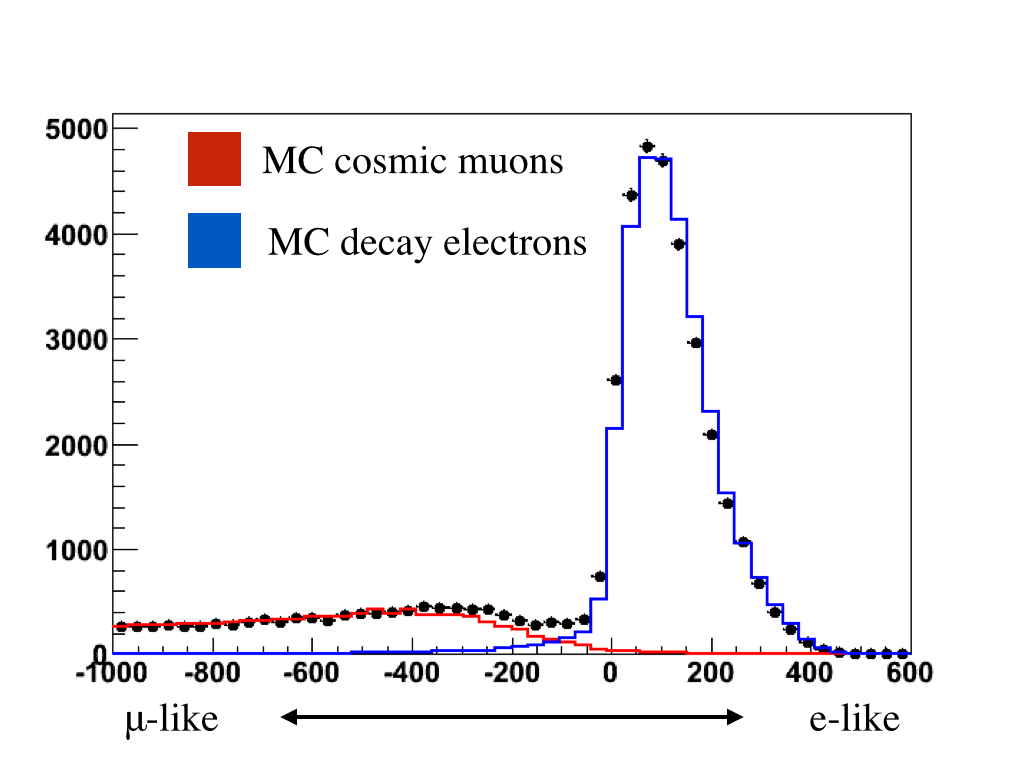
\includegraphics[width=0.6\textwidth]{cosmic_shift}
%  \end{center}
%  \caption{Distributions of the fiTQun $e/\mu$ PID parameter for MC stopping
%  cosmic muons (red) and the associated decay electrons (blue). Black points
%  show the observed data normalized to the MC\@. A shift in the distributions
%  between data and MC can be seen in both samples.}
%  \label{fig:shift}
%\end{figure}

The parameterization of detector uncertainties was chosen without detailed
knowledge of the actual data/MC discrepancies in the atmospheric data.  This
was done to ensure that the parameterization is not tuned to specific
discrepancies in the atmospheric data, which may arise from statistical
fluctuations or other sources besides the mis-modeling of detector parameters
that we are trying to measure.  



%-----------------------------------------------------------------------------
% Flux and Xsec Parameters
%-----------------------------------------------------------------------------
\subsection{Atmospheric Flux and Cross Section Parameterization}
\label{subsec:alphapar}

One difficulty in using atmospheric neutrino data to constrain SK detector
systematics is that the true distributions of the neutrino energy spectrum, the
flavor composition, and the interaction modes are not known precisely.  This is
due to the fact that there are significant uncertainties in the flux and cross
sections for atmospheric neutrino events.  Ideally, we wish to separate the
contributions of the flux and cross section uncertainties from the detector
systematic uncertainties, so that we may propagate only the components that
directly affect the T2K analyses. 

In principle, the cross section uncertainties are also shared between the
atmospheric and T2K analyses, so these parameters should be fit jointly with
the T2K data. Indeed, for future analyses, it may be preferable to use the T2K
cross section parameterization, which would allow these parameters to be
jointly estimated using both T2K and atmospheric neutrino data. Such a unified
approach is the subject of ongoing study by the T2K-SK group. For this
particular analysis, however, we adopt the strategy from previous atmospheric fits of
simultaneously fitting the atmospheric flux, cross section, and detector
systematics parameters to the atmospheric data, and then propagating only the
detector uncertainties to the T2K analysis. 

\begin{figure}[h]
  \begin{center}
    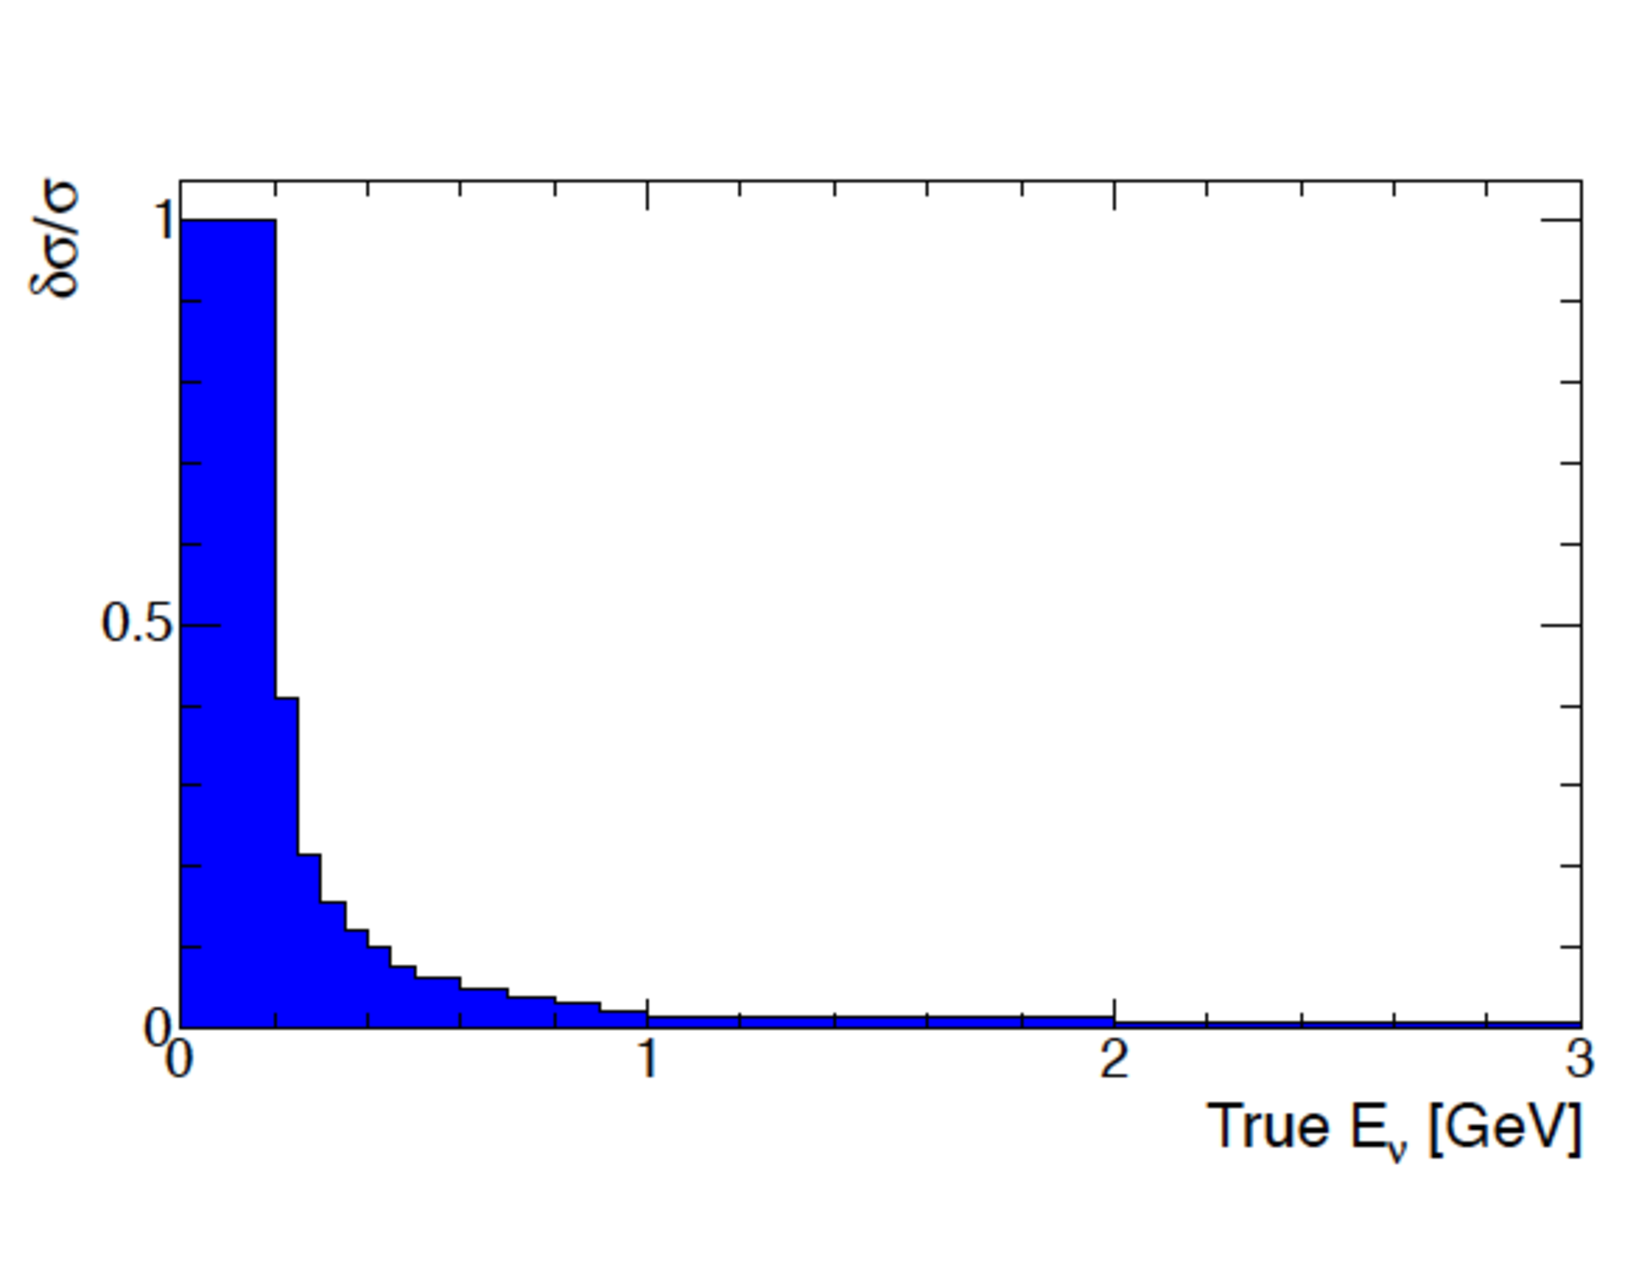
\includegraphics[width=0.5\textwidth]{tn186EnuXsec}
  \end{center}
  \caption{Dependence of the CCQE cross section uncertainty $\alpha_{CCQE}$ on
  the true neutrino energy.}
  \label{fig:alphaccqe}
\end{figure}

The parameterization of the atmospheric flux and cross section uncertainties in
this analysis is identical to that of TN-186~\cite{tn186}, which was in turn taken from
TN-157~\cite{tn157}, TN-159~\cite{tn159}, and TN-034~\cite{tn034}. The list of
flux and cross section parameters are shown in Table~\ref{tab:alpha}.  Each of
these 19 parameters are applied to the MC as a multiplicative factor that
affects only the events of the given ``Event Class'' in Table~\ref{tab:alpha}.

\begin{table}
  \centering
  \begin{tabular}{c c | c | c | c }
    \hline\hline
    n & Event Class & Parameter & Type & Prior Uncertainty $(\sigma_{\alpha})$ \\
    \hline 
    1 & $E_{\nu} <$ 1 GeV & $\alpha_{NormLowE}$ & Flux normalization & 0.25 \\
    1 & $E_{\nu} >$ 1 GeV & $\alpha_{NormHighE}$ & Flux normalization & 0.15 \\
    2 & CCQE & $\alpha_{CCQE}$ & Cross section & Figure~\ref{fig:alphaccqe} \\
    3 & CCnQE & $\alpha_{CCnQE}$ & Cross section & 0.20 \\
    4 & $\nu_{\mu}$ & $\alpha_{\nu_{mu}/\nu_{e}}$ & Cross section ratio & 0.05 \\
    5 & NC & $\alpha_{NC}$ & Cross section & 0.20 \\
    \hline\hline
  \end{tabular}
  \caption{Atmospheric flux and cross section parameters.  These parameter
  definitions are identical to those of T2K TN-186 Table 6. The event class is
  determined by cuts on the MC truth information.}
  \label{tab:alpha}
\end{table}




%-----------------------------------------------------------------------------
% MC Components
%-----------------------------------------------------------------------------
\subsection{MC Component Definitions}
\label{subsec:components}

The detector uncertainty parameters outlined in Section~\ref{subsec:betapar}
should be fit independently for different event topologies. The idea here is to
allow, for example, the events with a single muon ring to have shifts in the
reconstructed fiTQun quantities that are independent of the events with a
single electron ring.  To facilitate this, the MC is broken down into various
``components'', with each component containing a different visible event
topology that in principal could exhibit a different shift between the data and
simulation.  When defining the MC components, a balance must be struck between
accounting for many different topologies and having enough data statistics to
provide a constraint on it's distribution shapes.  The component definitions
chosen for this analysis are shown in Table~\ref{tab:components}.  These
components are defined purely in terms of their visible rings (as opposed to
the underlying interaction mode or particle type) since fiTQun is directly
sensitive to this information.  The visible rings are counted by iterating
through the simulated particles that exit the nucleus and identifying those
that are above the Cherenkov threshold ($\beta > \frac{1}{n})$.

\begin{table}
  \centering
  \begin{tabular}{c | c | l }
    \hline\hline
    MC Component $k$ & Name & Definition (from MC truth) \\
    \hline
    0 & Single Electron & Single visible electron ring \\
    1 & Single Muon & Single visible muon ring  \\
    2 & Electron-like + Other & Visible electron ring with other visible rings  \\
    3 & Muon-like + Other & Visible muon ring with other visible rings  \\
    4 & Single $\pi^{0}$ & Single visible $\pi^{0}$  \\
    5 & Single Hadron &Single visible proton or pion  \\
    \hline\hline
  \end{tabular}
  \caption{Definitions of the MC components that are used in the atmospheric
  fit.  Each component is defined based on the true visible topology. Each of these
  components receives a separate set of the $\beta$ parameters described in
  Section~\ref{subsec:betapar}. }
  \label{tab:components}
\end{table}



%-----------------------------------------------------------------------------
% Detector Regions
%-----------------------------------------------------------------------------
\subsection{Detector Region Definitions}
\label{subsec:DR}

To accomplish the goal of estimating detector systematics in various SK
detector regions, we further separate the MC events by their location and
orientation in the SK detector volume.  We define a particular event's location
and orientation in terms of two variables: \wall and \towall.  Here \wall
refers to the minimum distance between the particle vertex and the ID wall, and
\towall refers to the distance along the reconstructed particle track to the ID
wall.  The definitions are sketched out in Figure~\ref{fig:fvdiag}.

\begin{figure}[h]
  \begin{center}
    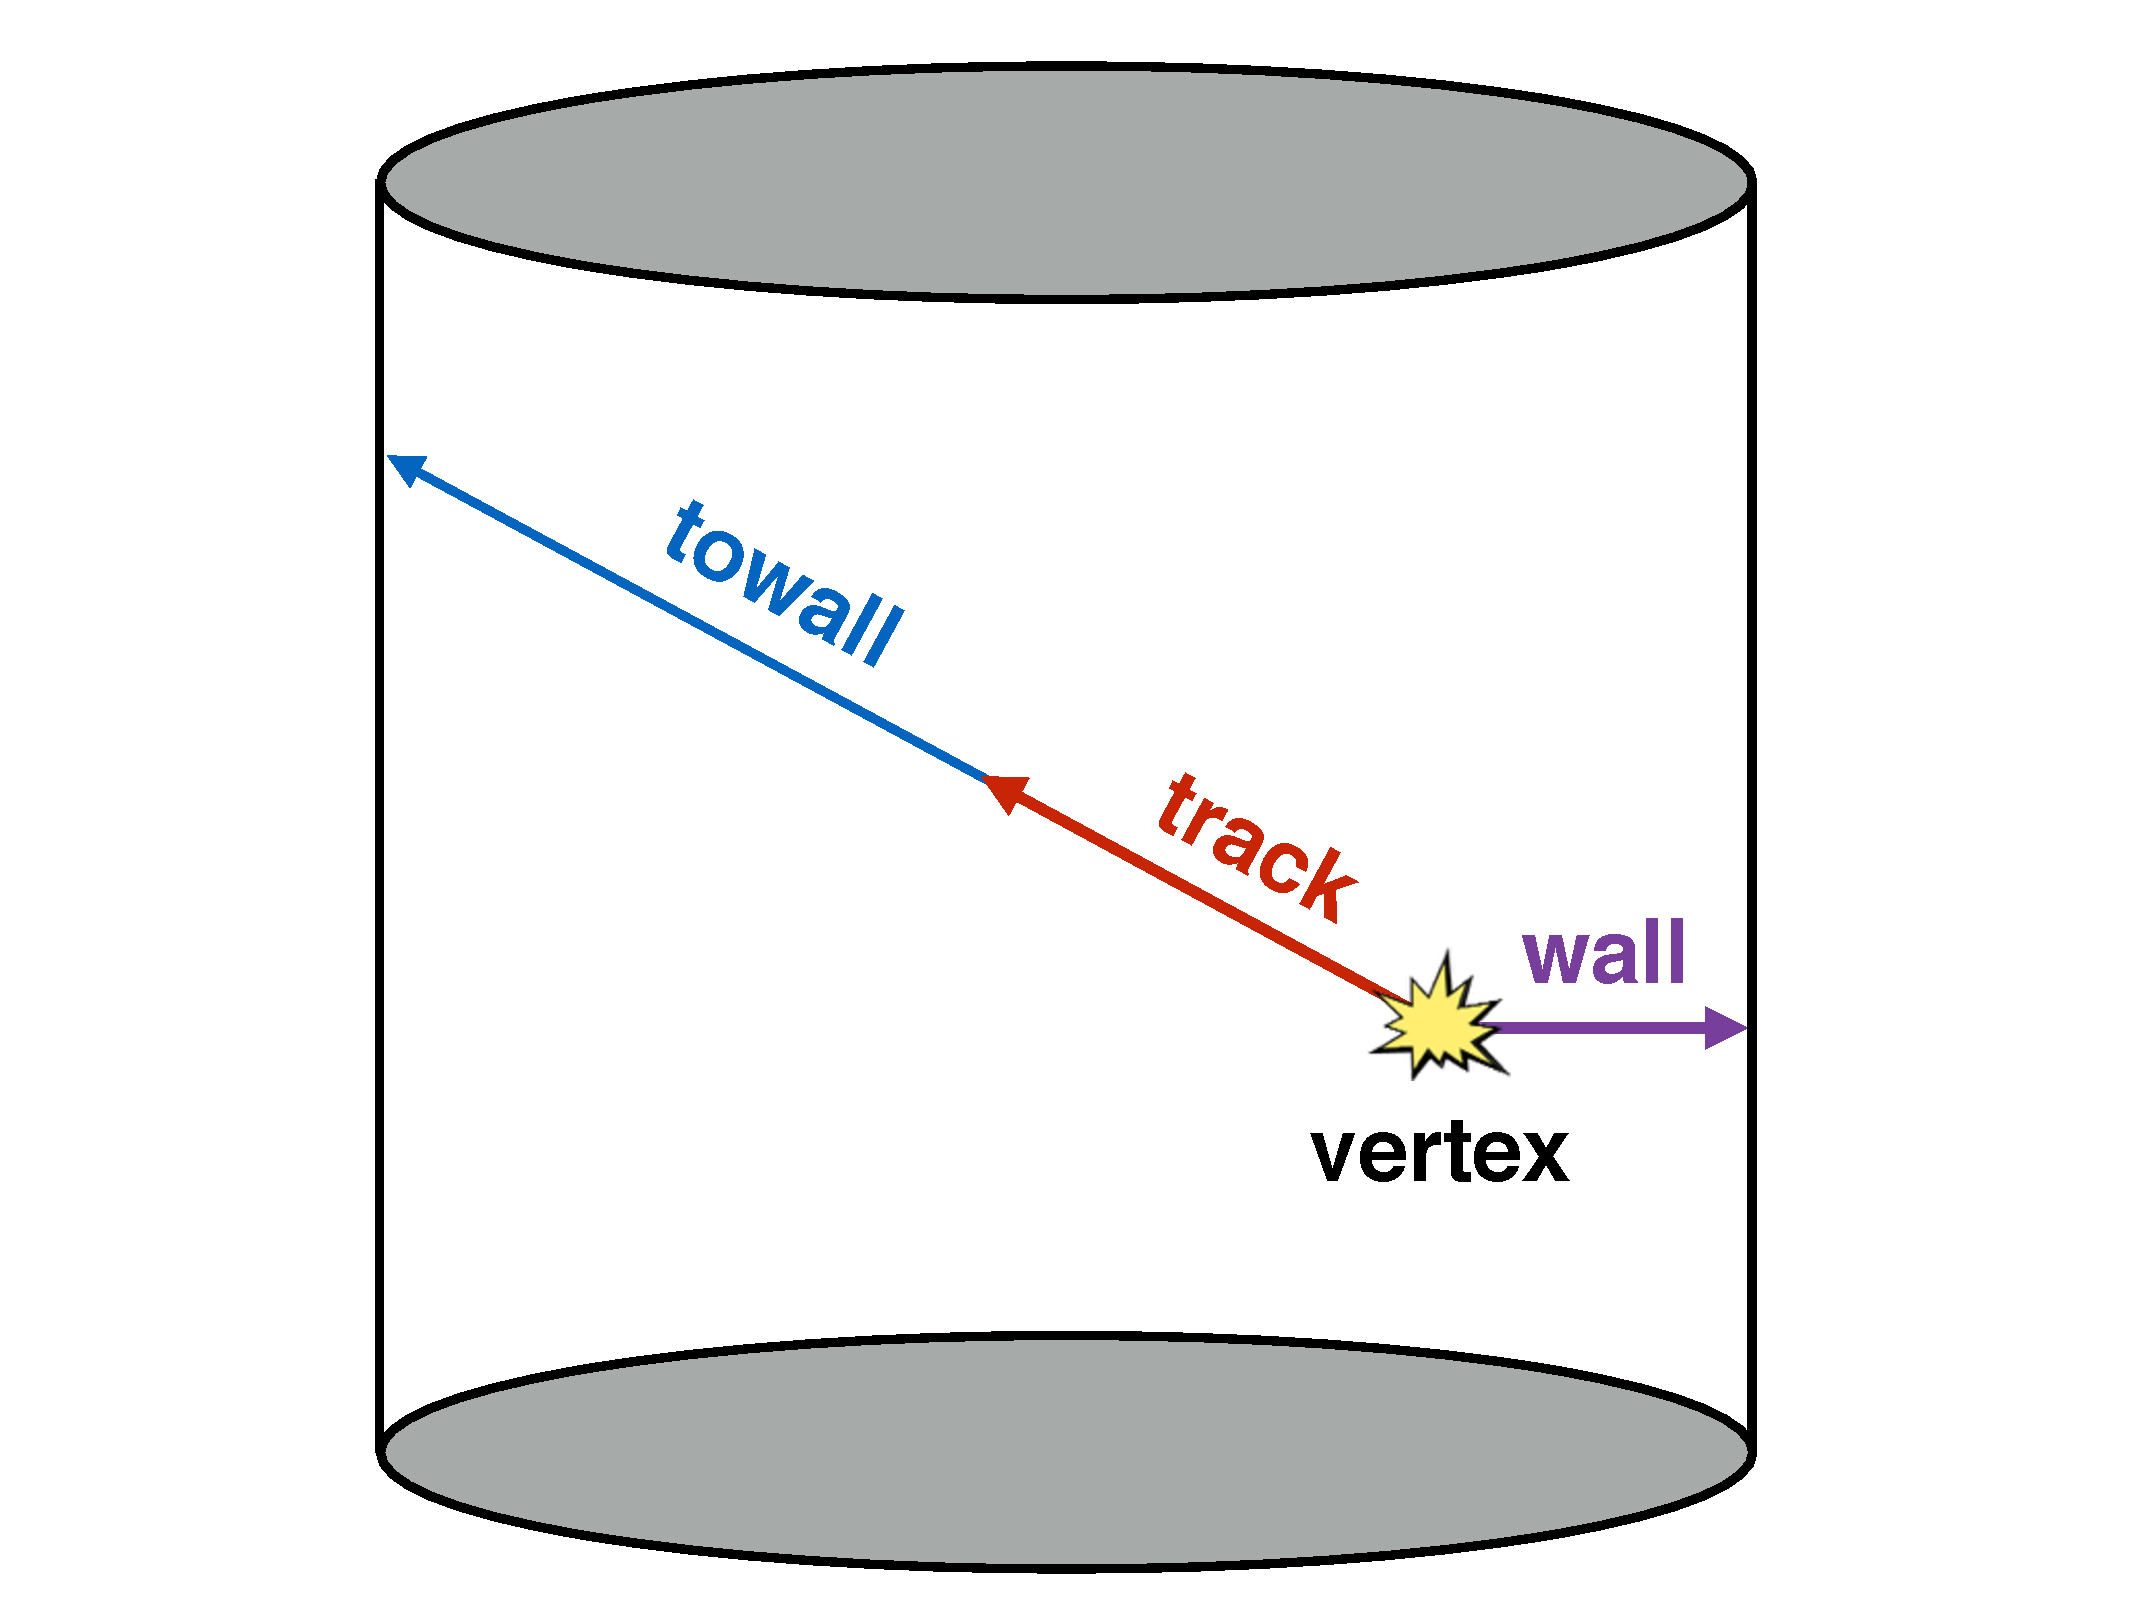
\includegraphics[width=0.5\textwidth]{wall_towall_def}
  \end{center}
  \caption{Graphical illustration of the definitions of the \wall and \towall variables
  that are cut on for the fiTQun FV cuts.  The \wall variable is the minimum distance between
  the reconstructed vertex and the ID wall, and the \towall variable is the distance along the 
  reconstructed particle track to the ID wall.}
  \label{fig:fvdiag}
\end{figure}

By discriminating events based on these two variables, we hope to better
isolate events that have poorly imaged Cherenkov rings from those with
well-imaged rings. Events that are close to the ID wall, but point inwards
(small \wall but large \towall), generally hit enough tubes to have a
well-imaged Cherenkov ring.  On the other hand, events that are close to the ID
wall but point towards the wall (small \wall and small \towall), generally hit
too few PMTS, and as a result have poorly imaged Cherenkov rings and may have to
be cut from the T2K sample.

\begin{table}
  \centering
  \begin{tabular}{c | c | c | c | c}
    \hline\hline
    Detector Region $j$ & Min. \towall & Max. \towall & Min. \wall & Max. \wall \\
    \hline\hline
    0 & 0cm    & 300  cm  & 0    cm & 300 cm \\
    1 & 300 cm & 5000 cm  & 0    cm & 80   cm \\
    2 & 300 cm & 800  cm  & 80   cm & 200 cm \\
    3 & 800 cm & 5000  cm & 80   cm & 200 cm \\
    4 & 300 cm & 800  cm  & 200  cm & 800 cm \\
    5 & 800 cm & 5000  cm & 200  cm & 5000 cm \\
    \hline\hline
  \end{tabular}
  \caption{Definitions of the detector region bins in terms of \wall and \towall.}
  \label{tab:fvbins}
\end{table}

\begin{figure}
  \begin{center}
    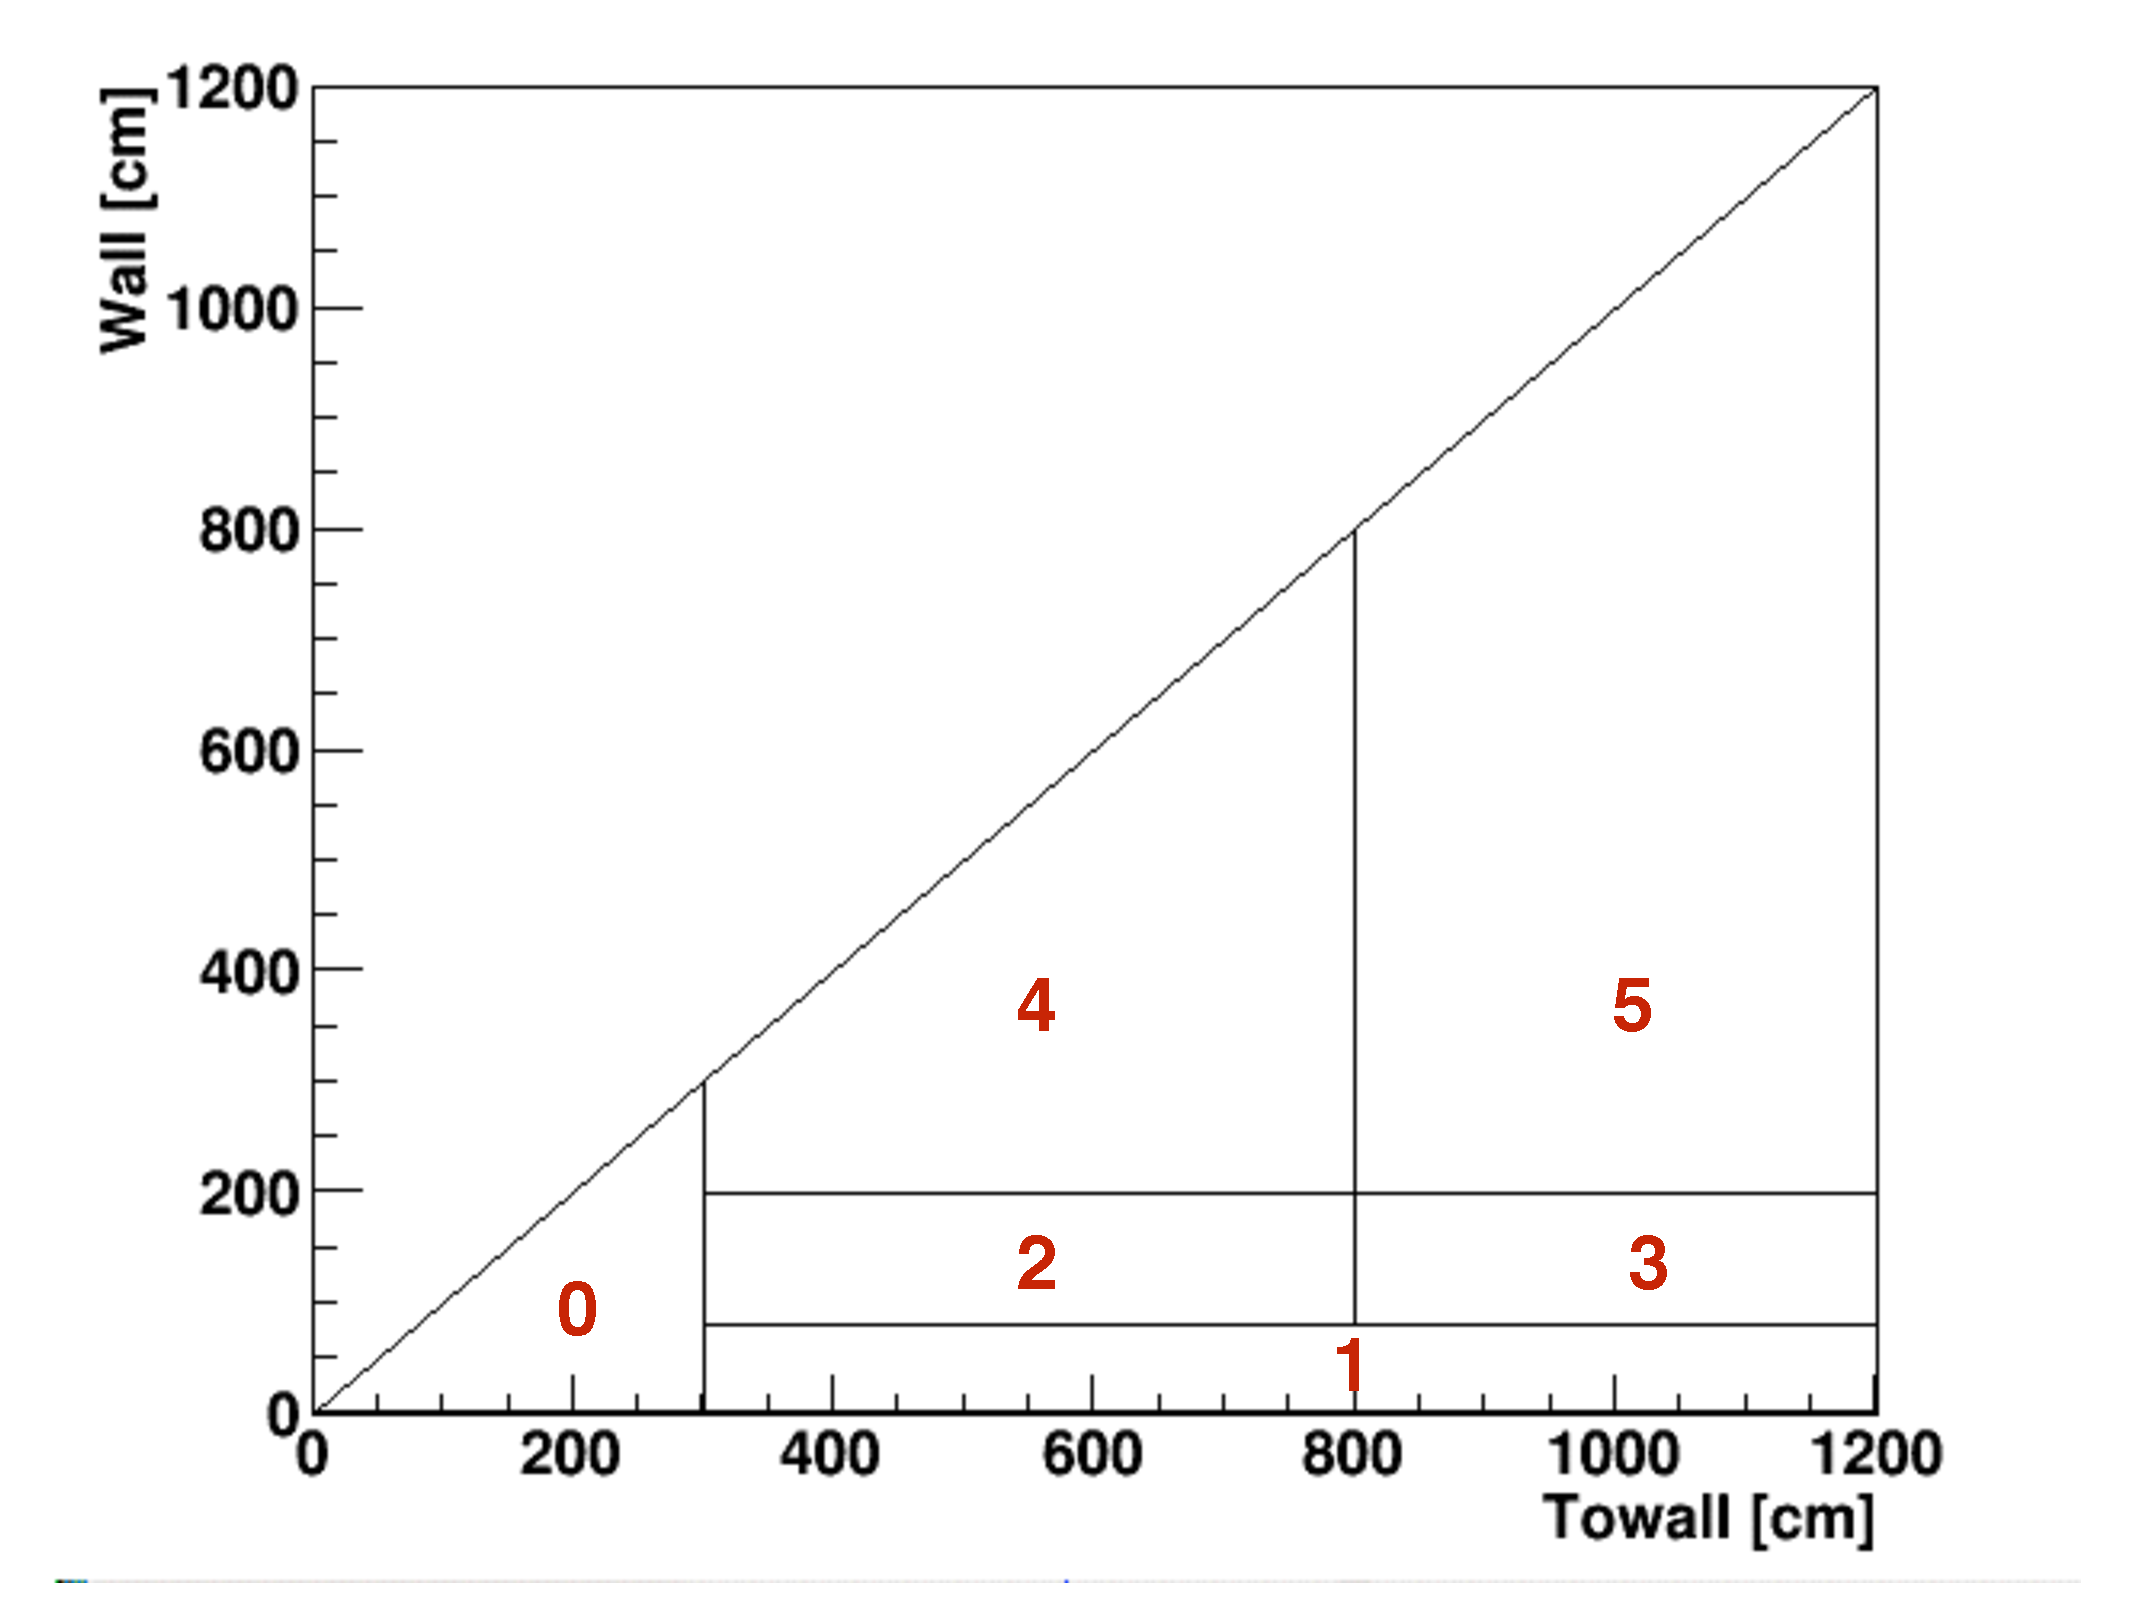
\includegraphics[width=0.5\textwidth]{plt_fvbins_labeled.pdf}
  \end{center}
  \caption{Graphical depiction of the detector region bins in terms of \wall
  and \towall.  Note that this plot is zoomed in on the small \wall and small
  \towall region.}
  \label{fig:fvbindef}
\end{figure}

A precise optimization of the fiTQun FV cuts requires knowledge of the SK
detector systematics in various regions of \wall and \towall.  To obtain this
information, we break up the $(towall,wall)$ space into bins and fit the
detector systematics in each bin separately.  The nominal binning in
\wall-\towall space is listed in Table~\ref{tab:fvbins} and shown in
Figure~\ref{fig:fvbindef}.  This binning was chosen to provide sensitivity to
how the systematic uncertainties change in key detector regions, while also
providing enough data statistics in each bin to constrain the parameters that
describe the uncertainties.  The events with both small \wall and small
\towall, (less than 300 cm) are isolated in the $j = 0$ FV bin.  Entering
background events, and events with poor energy reconstruction are almost
completely contained in the $j = 1$ FV bin.  The remaining region that with
\wall $< 200cm$ is divided into two \towall bins.  Each bin in
Figure~\ref{fig:fvbindef} will receive an independent set of $\beta$ parameters
that describe the fiTQun distribution shapes as described in
Section~\ref{subsec:betapar}.




%-----------------------------------------------------------------------------
% Data Samples
%-----------------------------------------------------------------------------
\subsection{Data and MC Sample Definitions}
\label{subsec:samples}

The MC components described in Section~\ref{subsec:components} are obtained from
cuts on the true visible event topology.  To fit these different components to
the atmospheric data, we must define another set of cuts on reconstructed quantities
that can be applied to both data and MC simulation.  The goal is to 
separate out the differnt MC components, but ideally we should not
use the fiTQun cut variables (such particle ID or ring-counting) whose
uncertainties we are trying to measure.  We choose instead to break down the
data and MC into broad samples based on the number of decay electrons, as listed
in Table~\ref{tab:samples}.  The sample with no decay electrons emphasizes the
single ring electron component, while the single decay electron sample
emphasizes the single ring muon and multi-ring electron components. An
additional sample for multiple decay electrons emphasizes the multi-ring muon
components.  By dividing up the data and MC in this way, we hope to achieve better
resolution of the systematic error uncertainties for each individual component.
Examples of how the MC components are distributed in each sample can be seen in
Figure~\ref{fig:samplot0} through Figure~\ref{fig:samplot2}.

Since the shifts in the fiTQun likelihood distributions should be independent of the
number of sub-events, we do not assign independent systematic error parameters
based on these samples. Instead, we introduce an overall normalization
parameter for each sample, denoted as $\gamma_{j,l}$, that scales the total
number of events for the $l$-th sample in the $j$-th detector region bin.  The systematic 
uncertainties associated with the decay electron tagging efficiency have been
evaluated with a a separate study on stopping cosmic muon data and are
described in TN-217~\cite{tn317}.

\begin{table}
  \centering
  \begin{tabular}{c | c}
    \hline\hline
    Sample $l$ & Cut \\
    \hline
    1 & fqnse = 1 \\
    2 & fqnse = 2 \\
    3 & fqnse $>$ 2 \\
    \hline\hline
  \end{tabular}
  \caption{The sample cuts that are applied to both data and MC events. The
  fqnse variable is the number fiTQun sub-events. The number of decay electrons
  is $fqnse -1$. }
  \label{tab:samples}
\end{table}


\begin{figure}[h!]
\centering
\begin{tabular}{l  l  l}
  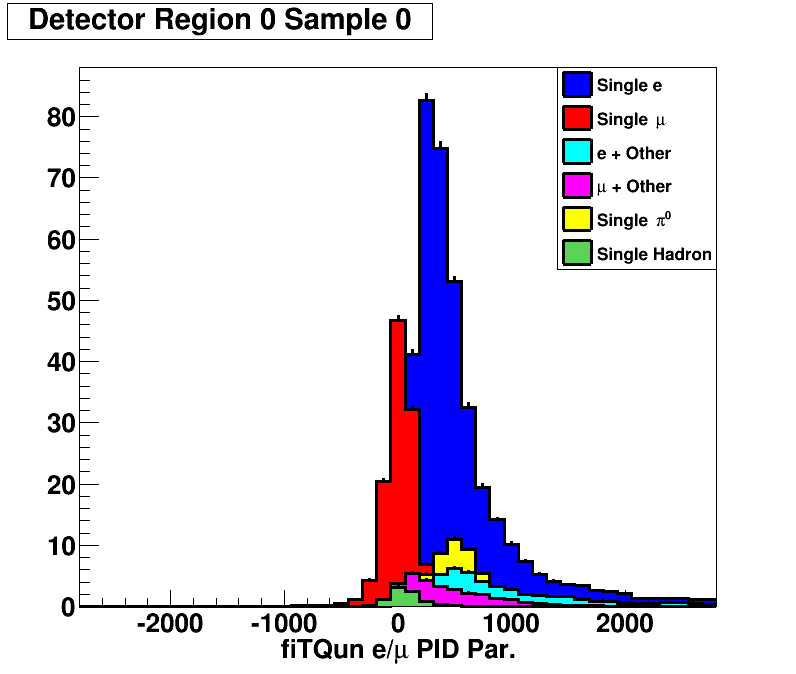
\includegraphics[width=0.33\textwidth]{plots/mc_breakdown_comp_0_bin_0_att_0} 
  &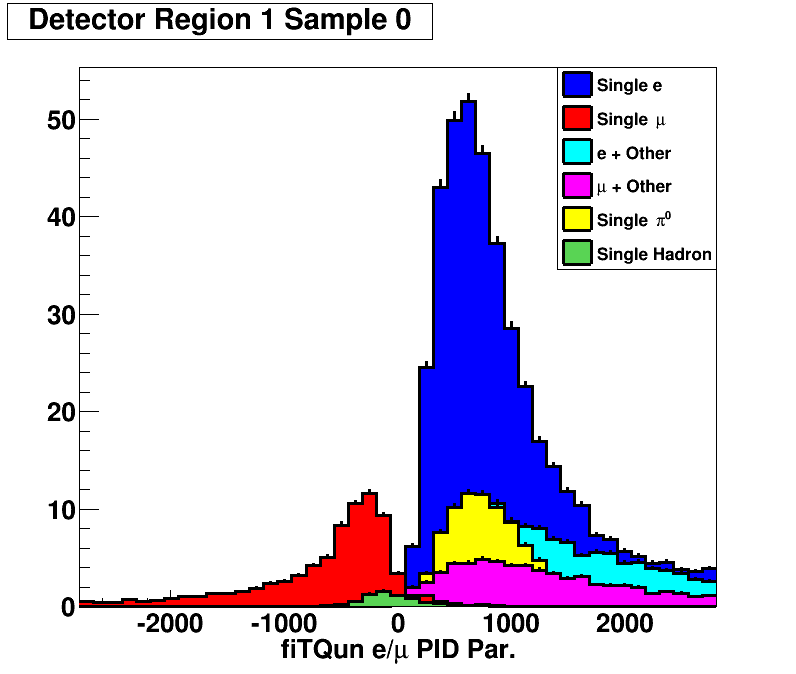
\includegraphics[width=0.33\textwidth]{plots/mc_breakdown_comp_0_bin_1_att_0}  
  &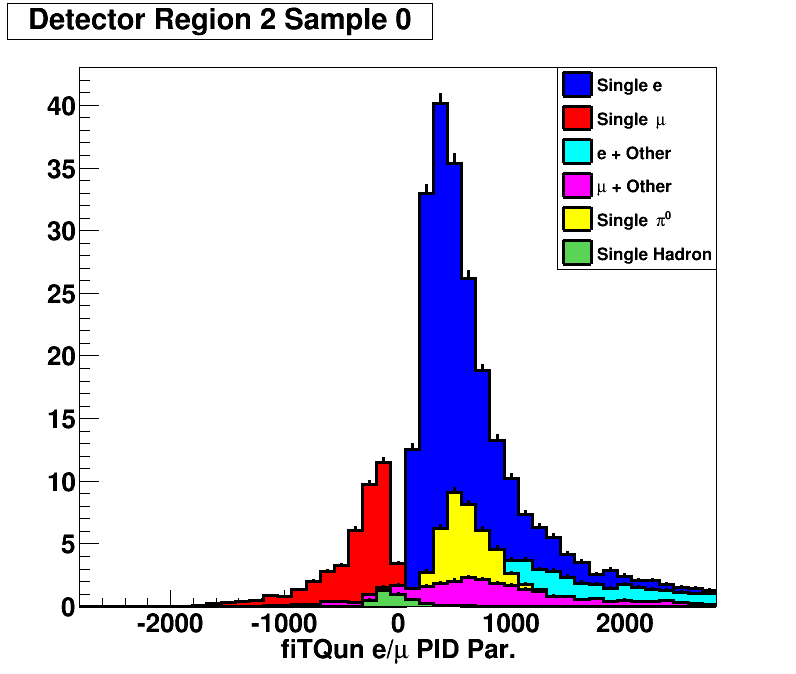
\includegraphics[width=0.33\textwidth]{plots/mc_breakdown_comp_0_bin_2_att_0} \\
  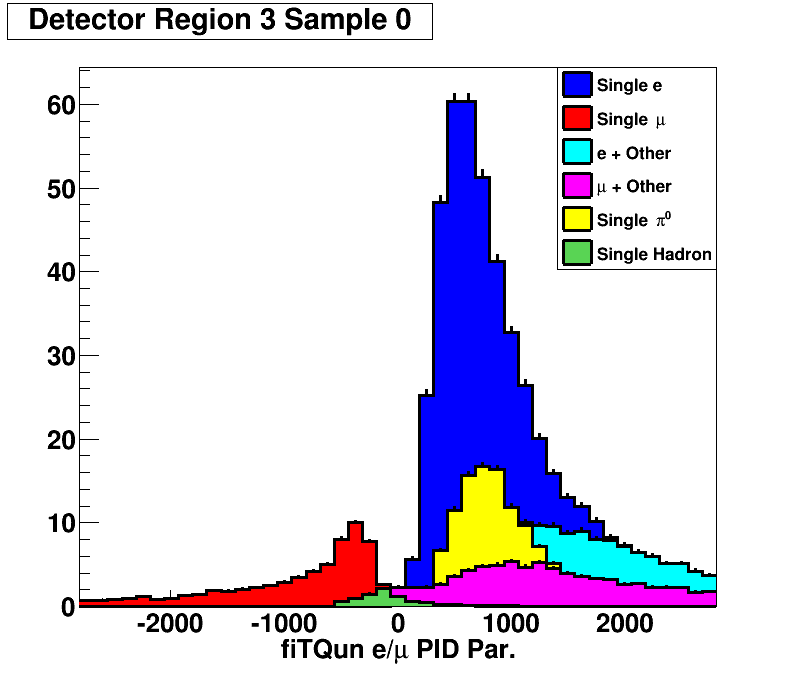
\includegraphics[width=0.33\textwidth]{plots/mc_breakdown_comp_0_bin_3_att_0} 
  &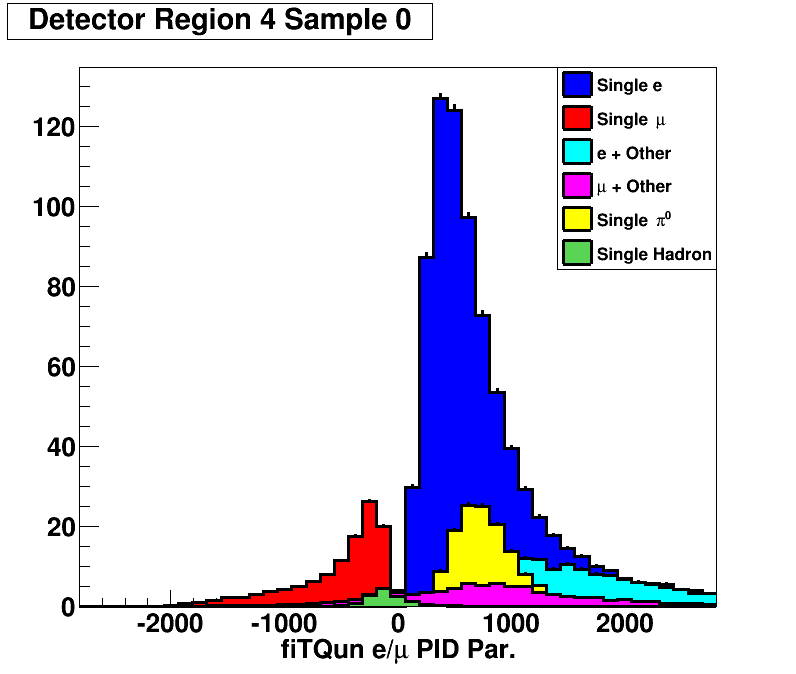
\includegraphics[width=0.33\textwidth]{plots/mc_breakdown_comp_0_bin_4_att_0} 
  &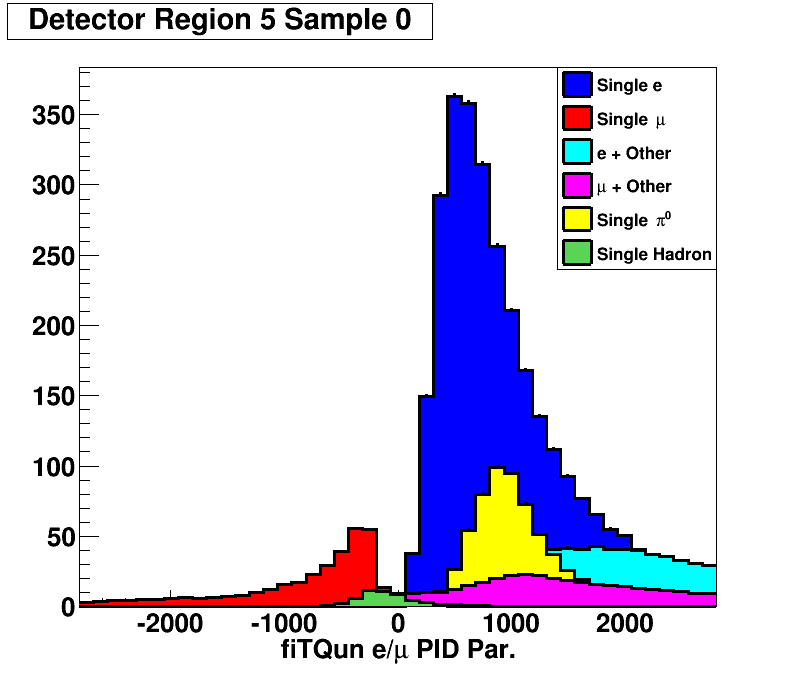
\includegraphics[width=0.33\textwidth]{plots/mc_breakdown_comp_0_bin_5_att_0}  
\end{tabular}
\caption{MC distributions of the fiTQun $e/\mu$ PID parameter for the $l = 0$
sample (no decay electrons) in all of the detector regions described in
Section~\ref{subsec:DR}.  In this sample, the single ring electron component
(defined in Section~\ref{subsec:components}) is emphasized. 
\towall.}
\label{fig:samplot0}
\end{figure}

\begin{figure}[h!]
\centering
\begin{tabular}{l  l  l}
  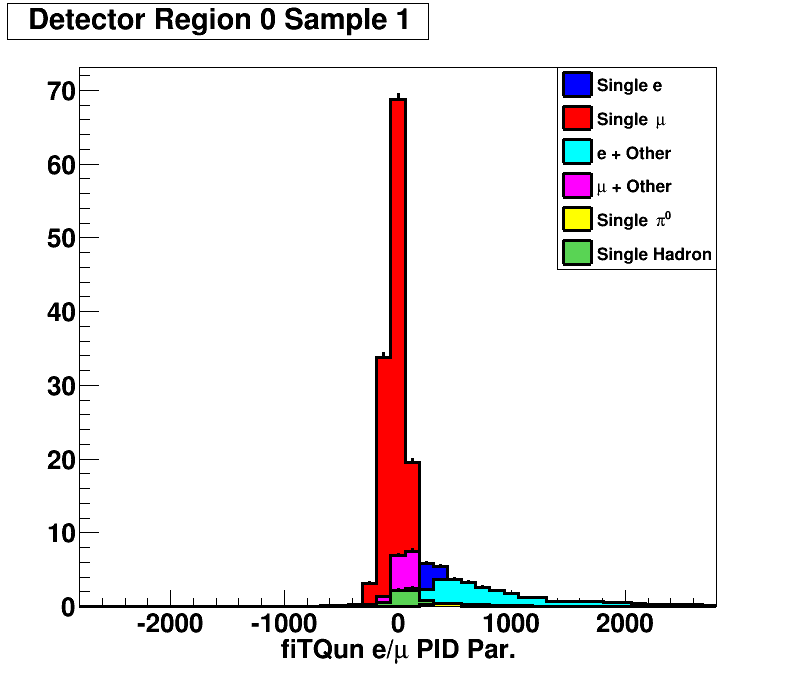
\includegraphics[width=0.33\textwidth]{plots/mc_breakdown_comp_1_bin_0_att_0} 
  &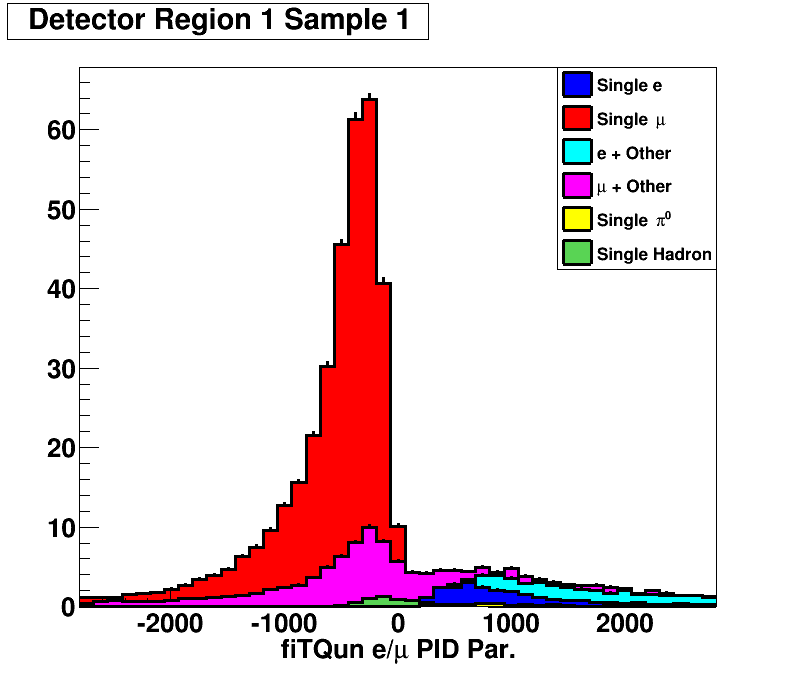
\includegraphics[width=0.33\textwidth]{plots/mc_breakdown_comp_1_bin_1_att_0}  
  &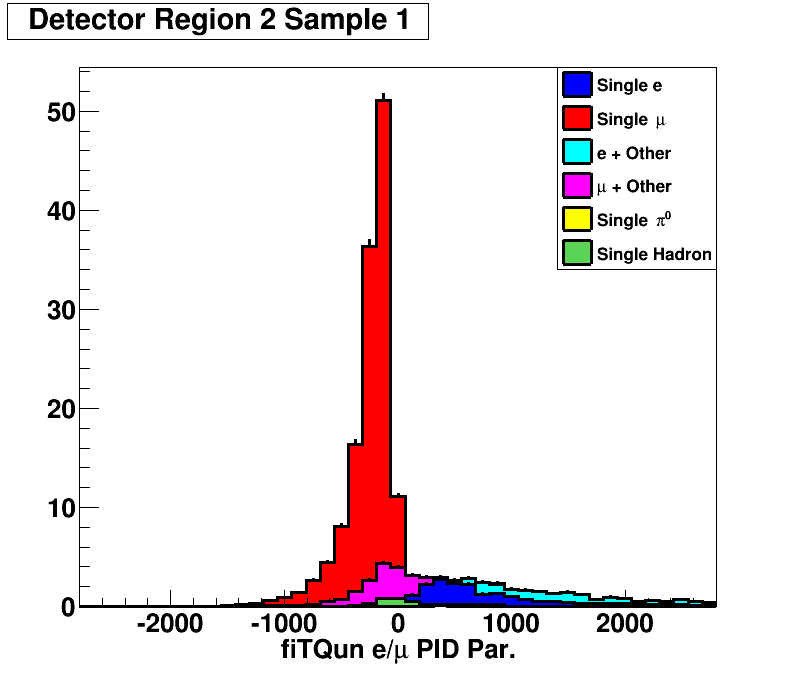
\includegraphics[width=0.33\textwidth]{plots/mc_breakdown_comp_1_bin_2_att_0} \\
  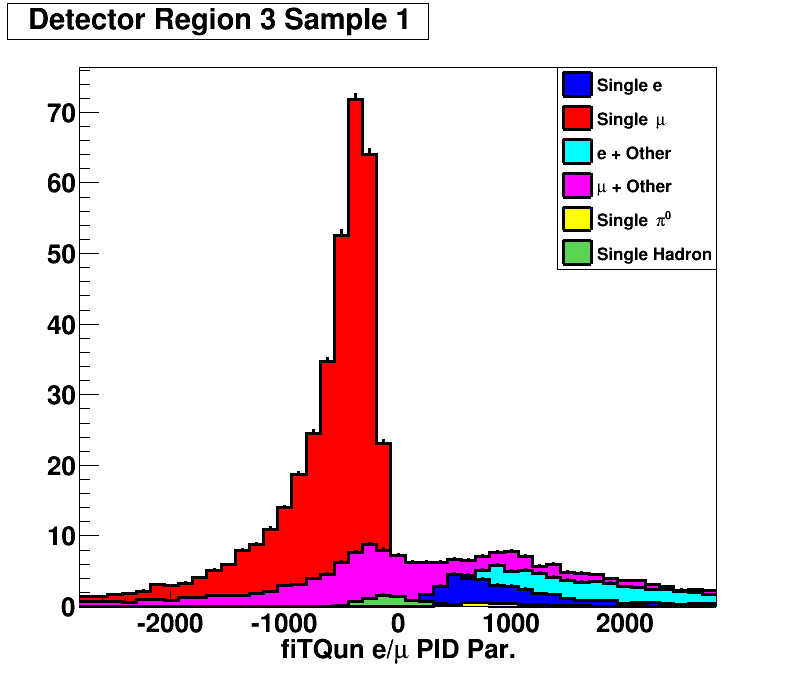
\includegraphics[width=0.33\textwidth]{plots/mc_breakdown_comp_1_bin_3_att_0} 
  &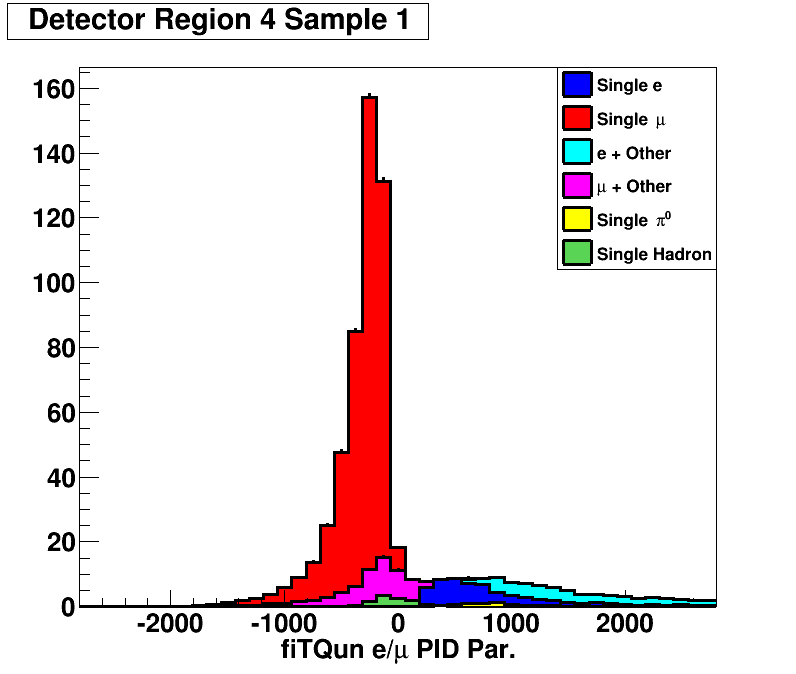
\includegraphics[width=0.33\textwidth]{plots/mc_breakdown_comp_1_bin_4_att_0} 
  &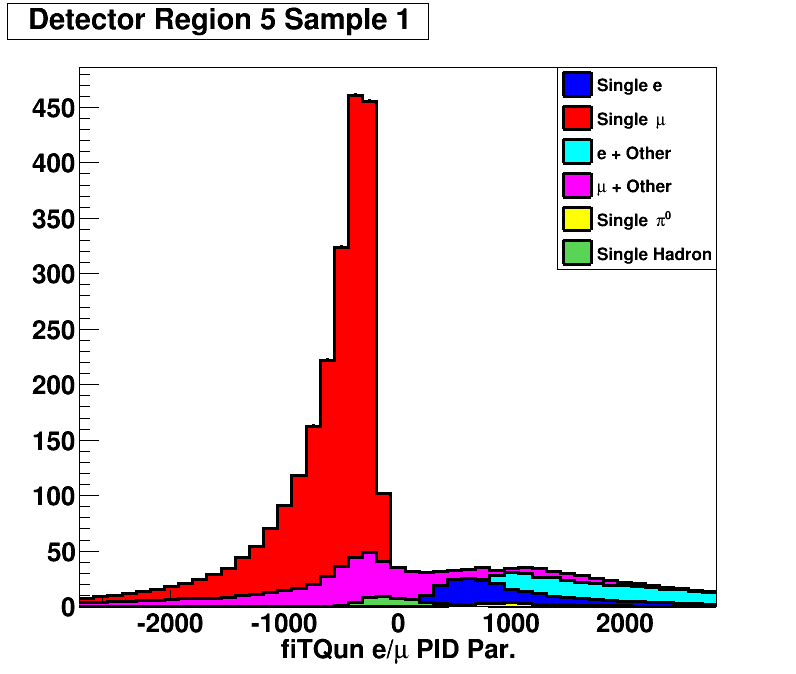
\includegraphics[width=0.33\textwidth]{plots/mc_breakdown_comp_1_bin_5_att_0} 
\end{tabular} 
\caption{MC distributions of the fiTQun $e/\mu$ PID parameter for the $l = 1$
sample (one decay electron) in all of the detector regions described in
Section~\ref{subsec:DR}.  In this sample, the single ring muon and multi-ring
electron components (defined in Section~\ref{subsec:components}) are
emphasized.}
\label{fig:samplot1}
\end{figure}

\begin{figure}[h!]
\centering
\begin{tabular}{l  l  l}
  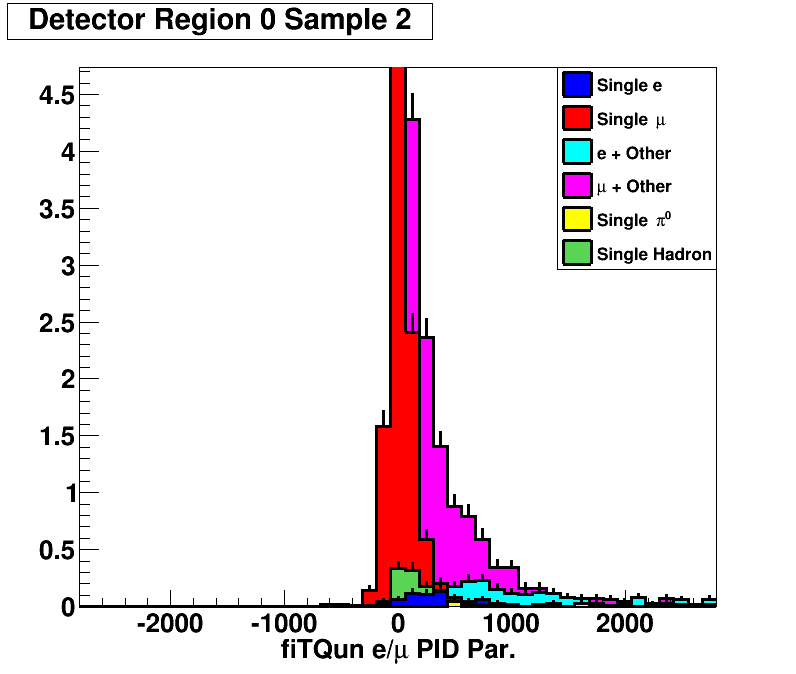
\includegraphics[width=0.33\textwidth]{plots/mc_breakdown_comp_2_bin_0_att_0} 
  &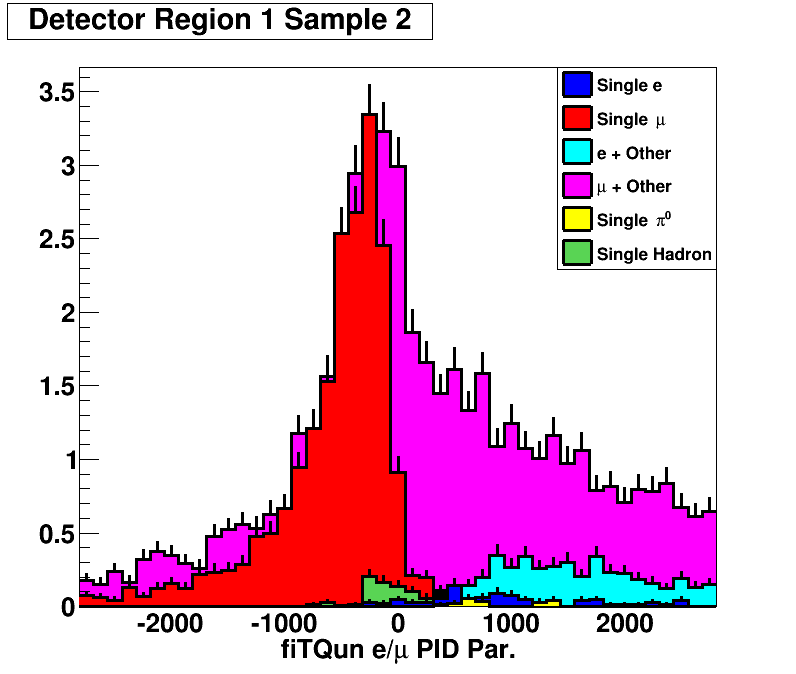
\includegraphics[width=0.33\textwidth]{plots/mc_breakdown_comp_2_bin_1_att_0}  
  &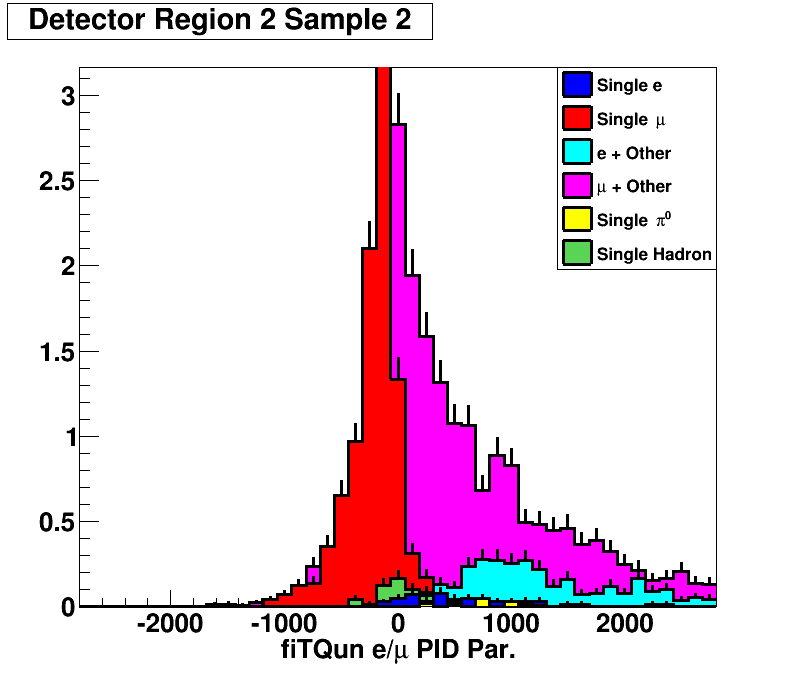
\includegraphics[width=0.33\textwidth]{plots/mc_breakdown_comp_2_bin_2_att_0} \\
  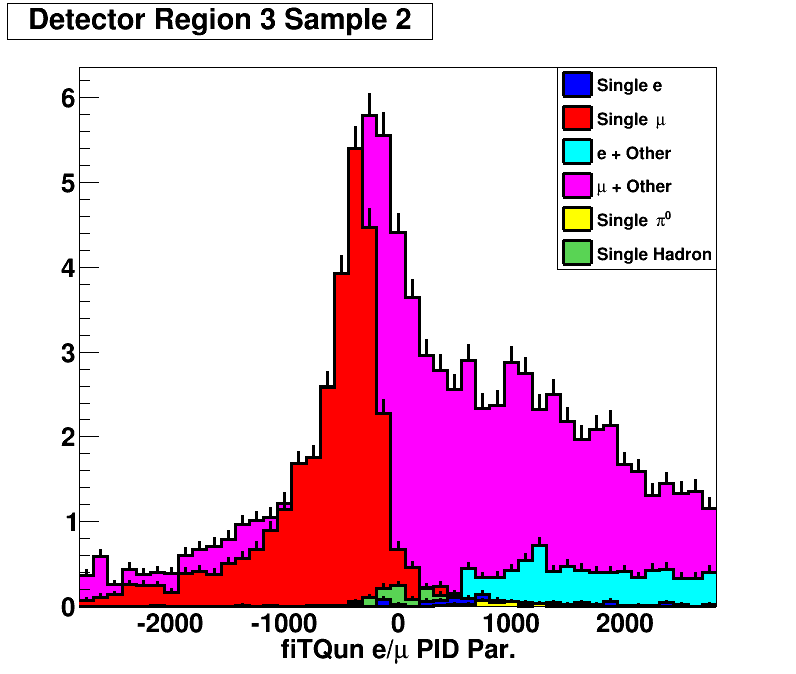
\includegraphics[width=0.33\textwidth]{plots/mc_breakdown_comp_2_bin_3_att_0} 
  &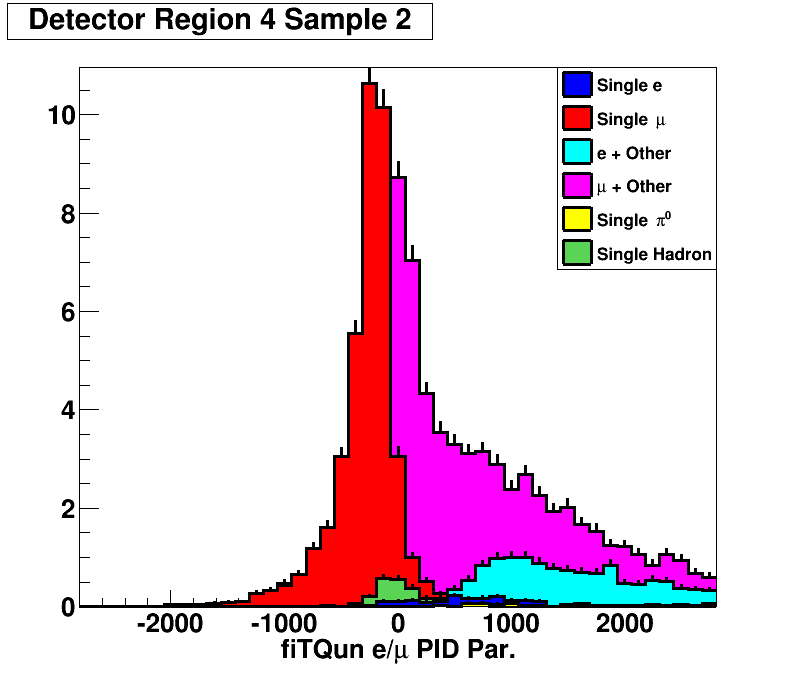
\includegraphics[width=0.33\textwidth]{plots/mc_breakdown_comp_2_bin_4_att_0} 
  &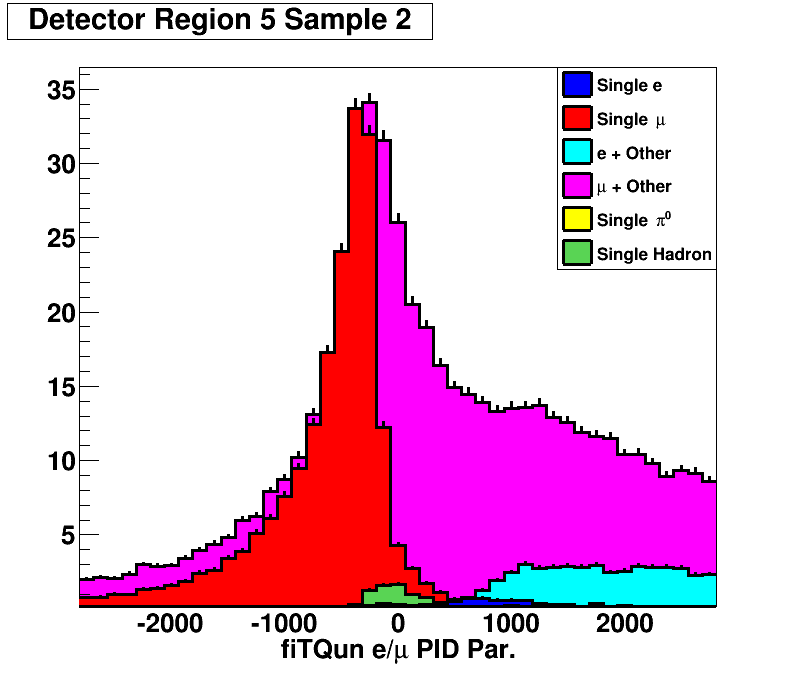
\includegraphics[width=0.33\textwidth]{plots/mc_breakdown_comp_2_bin_5_att_0} 
\end{tabular} 
\caption{MC distributions of the fiTQun $e/\mu$ PID parameter for the $l=2$ 
sample (more than one decay electron) in all of the detector regions described in
Section~\ref{subsec:DR}.  In this sample, the multi-ring muon component
(defined in Section~\ref{subsec:components}) is emphasized.}
\label{fig:samplot2}
\end{figure}
\FloatBarrier




%-----------------------------------------------------------------------------
% Full Parameterization
%-----------------------------------------------------------------------------
\subsection{Full Fit Parameterization}
\label{subsec:fullpars}

The full parameterization for the atmospheric fit is defined in terms of the MC
components, the detector regions, and the flux and cross section parameters
described in the previous sections.  The fiTQun cut variables we wish to
estimate systematics for are listed in Table~\ref{tab:fqvars}. The full
parameterization of the detector systematics is then the following set of
parameters:

\begin{equation}
  \label{eq:fullpars}
  \{\alpha_{n}, \beta_{j,k,m}^{i}, \gamma_{j,l} \}
\end{equation}

Where $i \in \{0,1\}$ denotes the additive or multiplicative shape parameter
described in Section~\ref{subsec:betapar}, $j \in \{0,1,2,3,4,5\}$ denotes the
detector region bin, $k \in \{0,1,2,3,4,5\}$ denotes the MC component described
in Section~\ref{subsec:components},  $l \in \{0,1,2\}$ denotes the sample
described in Section~\ref{subsec:samples}, and $m \in \{0,1,2,3\}$ denotes the
fiTQun cut variable in Table~\ref{tab:fqvars}. 

There are 288 of the $\beta$ parameters in total.  These parameters are fit
simultaneously with the atmospheric flux and cross section parameters
$\alpha_{n}$ (19 parameters) and the sample normalizations $\gamma_{j,l}$ (18
parameters) for a total of 325 parameters in this fit.



%-----------------------------------------------------------------------------
% Likelihood Definition
%-----------------------------------------------------------------------------
\subsection{Parameter Likelihood Definition}
\label{subsec:parlike}

With the fit parameters described in previous sections, we now address the
details of how they are constrained by the SK atmospheric neutrino data.  In
previous atmospheric fits, such as the one described in TN-186, the parameters
are constrained by comparing the numbers of events that either pass or fail the
cuts on the reconstructed variables.  This amounts to essentially binning each
of the cut variables into two bins separated by the optimal cut chosen for the
T2K analysis.  We modify this approach by fitting to the full distributions
of the fiTQun cut variables listed in Table~\ref{tab:fqvars}.

There are several advantages to fitting to the entire cut variable
distributions.  One clear advantage is that this includes more shape
information in the fit, which should in principle provide better constraints on
the systematics for the MC components that dominate each distribution. This
point is particularly important for determining systematics in the small \wall
and small \towall detector regions, where the data statistics becomes a limiting
factor.  Another advantage is that this decouples the estimation of detector
systematics from the optimization of the cut values, since we no longer use the
T2K cut values explicitly in the fit.   

To formalize this concept, we define $\mathbf{h}^{MC}$ to be the set of
histograms $h^{MC}_{j,l,m}$ filled from MC for all values of $j$, $l$, and $m$,
where again $j$  is the detector region bin, $l$ is the sample based on the
number of decay electrons, and $m$ is the index of the fiTQun topological cut
variable from Table~\ref{tab:fqvars}.

Similarly, we define $\mathbf{h}^{Data}$ as the set of histograms
$h^{Data}_{j,l,m}$ filled using SK atmospheric data. We consider $
\mathbf{h}^{Data}$ to be the observed data $\mathbf{M}_{Atm-Sk}$ in
Equation~\ref{eq:likelihood}, and the previously defined detector systematic
parameter sets $\beta$, and normalizations $\gamma$ to be \ldsk, and finally
the flux and cross section parameters $\alpha$ from
Section~\ref{subsec:alphapar} to be $\mathbf{a}$ and $\mathbf{x}_{atm}$.  We can now define the
negative log-likelihood from Equation~\ref{eq:likelihood} to be:
%
\begin{equation}
  \label{eq:loglikelihood}
  -log[\mathcal{L}(\alpha,\beta,\gamma | \mathbf{h}^{Data} )] =
  -log[P( \mathbf{h}^{Data} | \mathbf{h}^{MC}(\alpha,\beta,\gamma))] - log[\pi(\alpha)]
  - log[\pi(\beta,\gamma)]
\end{equation}
%
The first term on the right hand side can be expanded as a sum over the bins
$s$, assuming Poisson statistics in each bin:
%
\begin{gather*}
  \label{eq:logpoisson}
  -log[P( \mathbf{h}^{Data} | \mathbf{h}^{MC}(\alpha,\beta,\gamma))] = \\
    \sum\limits_{s}^{} \sum\limits_{j}^{} \sum\limits_{l}^{} \sum\limits_{m}^{} 
   \bigg[ (\hat{N}_{s,j,l,m}(\alpha,\beta,\gamma) - N_{s,j,l,m}) +
  N_{s,j,l,m}log\bigg(\frac{N_{s,j,l,m}}{\hat{N}_{s,j,l,m}(\alpha,\beta,\gamma)}\bigg)\bigg]
\end{gather*}
%
where $N_{s}$ denotes the observed contents of the histogram bin $s$, and
$\hat{N}_{s}$ denotes the MC expectation (assumed to be the Poisson mean) of
histogram bin $s$ given the values of the systematics parameters.  The
histogram bin widths, as well as the maximum and minimum values of the
histogram $x$-axis, were chosen to obtain reasonable data statistics in each
bin, as well as to emphasize the regions near the T2K cut values, where any
shift will have the largest impact on the size and composition of the event
samples.  The exact histogram ranges and bin size can be seen most readily in 
Figures~\ref{fig:fitresults_samp0_att0}-~\ref{fig:fitresults_samp2_att3} found in 
Section~\ref{sec:fitresults}.

The remaining terms in the likelihood are the priors for each of the fit
parameters.  We assume each prior is a Gaussian shape with some width
$\sigma$ around the nominal parameter values.  For the atmospheric flux and
cross section parameters $\alpha$, we take $\sigma_{\alpha_{n}}$ to be the
values listed in Table~\ref{tab:alpha}.  For the detector systematics
parameters $\beta$ we assign the priors listed in Table~\ref{tab:betaprior}.
These priors are chosen to provide a loose constraint that does not dominate
over the constraints from data, but also to keep the parameters constrained
from moving to values that are much more extreme values.  We can then expand
the terms for the priors as:
%
\begin{gather*}
  \label{eq:logpriors}
  - log[\pi(\alpha)] - log[\pi(\beta,\gamma)] = \\ \frac{1}{2}
  \sum\limits_{n}^{} \bigg(\frac{(\alpha_{n} - 1)}{\sigma_{\alpha_{n}}}\bigg)^{2} +
   \frac{1}{2} \sum\limits_{j}^{} \sum\limits_{l}^{} 
  \bigg(\frac{(\gamma_{j,l} - 1)}{\sigma_{\gamma_{j,l}}}\bigg)^{2} + 
   \frac{1}{2} \sum\limits_{i}^{} \sum\limits_{j}^{} \sum\limits_{l}^{} \sum\limits_{m}^{}
  \bigg(\frac{(\beta_{j,l,m}^{i} - \delta_{i1})}{\sigma_{\beta_{m}}}\bigg)^{2}  
\end{gather*}
%
Putting of this all together, we wish to minimize the following negative log-likelihood, which is a
sum of $1,134$ terms:
%
\begin{equation}
 \begin{gathered}
  -log[\mathcal{L}(\alpha,\beta,\gamma | \mathbf{h}^{Data}  )] = \\
  \sum\limits_{s}^{} \sum\limits_{i}^{}  \sum\limits_{j}^{} \sum\limits_{l}^{} \sum\limits_{m}^{} \sum\limits_{n}^{}
  \bigg[ (\hat{N}_{s,j,l,m}(\alpha,\beta,\gamma) - N_{s,j,l,m})
    + N_{s,j,l,m}log\bigg(\frac{N_{s,j,l,m}}{\hat{N}_{s,j,l,m}(\alpha,\beta,\gamma)}\bigg) \\
  + \frac{1}{2}\bigg(\frac{(\alpha_{n} - 1)}{\sigma_{\alpha_{n}}}\bigg)^{2}
  + \frac{1}{2}\bigg(\frac{(\gamma_{j,l} - 1)}{\sigma_{\gamma_{j,l}}}\bigg)^{2} 
  + \frac{1}{2}\bigg(\frac{(\beta_{j,l,m}^{i} - \delta_{i1})}{\sigma_{\beta_{m}}}\bigg)^{2} \bigg] 
 \end{gathered}
 \label{eq:likefull}
\end{equation}


\begin{table}[h]
  \centering
  \begin{tabular}{c|c|c}
   \hline\hline
   Cut Variable $m$ & Variable Name & Prior Constraint $\sigma_{\beta_{m}}$ \\
   \hline\hline
   0 & $e/\mu$ PID & 200 \\
   1 & $e/\pi^{0}$ PID & 200 \\
   2 & $\mu/\pi$ PID & 200 \\
   3 & Ring-Counting &100 \\
   \hline\hline
  \end{tabular}
  \caption{Loose prior constraints assigned to the detector systematics parameters. The
  constraint values are dimensionless and reflect the scales of the fiTQun likelihood ratios
  for each variable.}
  \label{tab:betaprior}
\end{table}




%-----------------------------------------------------------------------------
% Likelihood Evaluation 
%-----------------------------------------------------------------------------
\subsection{Likelihood Evaluation}
\label{subsec:evalike}

While perhaps formally imposing, the likelihood defined explicitly in
Equation~\ref{eq:likefull} simply compares the data and MC by chopping the
events up into many histograms and then comparing data and MC in each bin.
This can be calculated numerically in a straightforward manner:

\begin{enumerate}
  \item \label{it:first} Fill a set of histograms of the fiTQun cut variables using the atmospheric data.
    There is a histogram for each cut variable, each detector region,
    and each control sample defined by the number of decay electrons.
  \item
    Fill a separate set of histograms using simulated data for some assumed
    values of the $\alpha$, $\beta$, and $\gamma$ parameters. There is a
    histogram for each fiTQun cut variable, each detector region, each control
    sample, \emph{and} each component defined by the true visible topology
  \item \label{it:sum} Sum the histograms of the MC components for each cut
    variable, each detector region, and each control sample. The resulting summed histograms
    does not depend on MC truth information and can be compared directly to data.
  \item
    \label{it:comp} Compare the MC summed histogram from Step~\ref{it:sum} to
    the corresponding data histogram, by evaluating the log-likelihood bin-wise
    as in Equation~\ref{eq:logpoisson}. 
  \item Add the contributions from the
    priors to the result of Step~\ref{it:comp} to obtain the final likelihood
    value from Equation~\ref{eq:likefull}.
\end{enumerate}

The steps outlined above can be repeated for different assumptions of the
systematics parameters to compare the relative likelihood of different
assumptions of systematics.  The goal now is to find the parameters that give
the best agreement to the data, i.e.\ the parameters that minimize the negative
log-likelihood.  Ideally, we would like to know not only the best-fit parameter
values, but also the preferred parameter regions and correlations.  To
accomplish this task, we use Markov chain Monte Carlo (MCMC) methods.



%-----------------------------------------------------------------------------
% MCMC Fit Methods
%-----------------------------------------------------------------------------
\subsection{MCMC Methods}
\label{subsec:mcmc}

MCMC is a stochastic technique that can be used to generate samples of detector
systematic parameters drawn from the likelihood defined in
Equation~\ref{eq:likefull}.  This is accomplished by essentially taking a
random walk through the parameter space and preferentially accepting steps
according to the likelihood definition. If we let $\theta$ denote the full set
of fit parameters, i.e.\ $\theta = (\alpha,\beta,\gamma)$, a MCMC run of length
N will produce a set of parameter values: $\{\theta_{1}, \theta_{1}, \dots
\theta_{N}\}$.  We can the sample from this set to obtain approximately
independent throws from the likelihood, which provides a powerful tool for
propagating uncertainties.  This is due to the fact that if we have some
quantity $X$ that depends on $\theta$ (such as the number of events passing
some set of selection criteria), we can easily calculate the expectation over
$\theta$ as as an average over some number $M$ of MCMC points:
%
\begin{equation}
  \label{eq:mcmcexp}
  \langle X \rangle_{\theta} = \frac{1}{M}\sum\limits_{i=0}^{M}X(\theta_{i})
\end{equation}
%
This expectation can then be compared to the nominal simulated value of $X$ to
quote a systematic uncertainty.

The MCMC in this fit uses the Metropolis-Hastings algorithm, described
in detail in the PDG and TN-140.  The procedure is as follows:

\begin{enumerate}
  \item Determine a distribution $Q(\theta|\theta_{0})$ that assigns a
    probability to each point $\theta$ given the current point $\theta_{0}$.
    This distribution should be symmetric under exchange of $\theta$ and
    $\theta_{0}$ so that $Q(\theta|\theta_{0}) = Q(\theta_{0}|\theta) $
  \item Choose an initial point  $\theta_{0}$
  \item Randomly select a proposed step according to $Q(\theta|\theta_{0})$.
  \item Calculate an acceptance probability $\Omega = min(1,\frac{P(\theta)}{P(\theta_{0})})$.
  \item Randomly select a point $u \in \{0, 1\}$ according to a uniform distribution.
  \item If $u<\Omega$, accept this proposal and return to Step 1 with $\theta_{0} = \theta$ 
  \item If $u>\Omega$, reject this proposal and return to Step 1 with $\theta_{0} = \theta_{0}$ 
\end{enumerate}

In practice, we first select an initial starting point $\theta_{0}$ by
minimizing the likelihood using MINUIT\@.  We then profile the likelihood for
each fit parameter $\theta^{i}$ to obtain a rough estimate of how sensitive the
likelihood is to changes in $\theta^{i}$.  The width of this likelihood profile
is then used to build a proposal distribution $Q(\theta|\theta_{0})$ that
throws each parameter independently from a Gaussian distribution centered on
$\theta^{i}_{0}$ and with a width determined by the 1D likelihood profile.

One potential drawback of using the proposal distribution
$Q(\theta|\theta_{0})$ described above is that it treats all parameters
independently and ignores potential correlations between the parameters.  In
the limit of infinite MCMC steps, this is not a problem, since the proposal
function will eventually ``guess'' all of the parameter combinations.  With a
finite chain, however, the presence of strong correlations between the fit
parameters may result in the chain not fully exploring the space of allowed
parameters, since some specific combinations that agree well with the data may
end up not be sampled by the proposal function in time.

The issue of strongly correlated parameters is particularly problematic for
this analysis due to our choice of detector error parameterization.  By
examining how the $\beta$ parameters are applied (see
Equation~\ref{eq:fqparmod}), it is clear that if the fiTQun variable $L_{m}$ is
not distributed around $0$, then a change in the multiplicative parameter
$\beta^{1}$ will also produce a shift which modifies the distribution in the
same manner as a change in $\beta^{0}$.  This redundancy results in strong
correlations between the $\beta^{0}$ and $\beta^{1}$ parameters.

One way to deal with this issue is to modify the proposal function to include
the expected parameter correlations.  There are many ways to approach this
problem, but one elegant way is to borrow the ideas from Differential Evolution
Markov Chain Monte Carlo (DE-MCMC).  A description of the algorithm can be
found in, for example, the Braak2006~\cite{Braak2006}. The strategy adopted
here is to run an initial MCMC and record the difference $\Delta \theta$ in the
parameters between each accepted point and some previously accepted point. The
result is a sampling of the preferred directions in the parameter space. One
can then sample from this list of preferred directions to build a proposal
function that includes all of the relevant correlations.  The overall approach
is as follows:
%
\begin{enumerate}
  \item Run an initial Metropolis-Hastings MCMC to obtain a set of the
    accepted point differences.  
  \item Choose a random element $\Delta \theta$ from the set of accepted point
    differences generated in Step 1.
  \item Choose a random perturbation $\delta$ (should be small compared to the characeristic
    $\Delta \theta$ step size).
  \item Given some initial point $\theta_{0}$ propose the next point $\theta$
    according to: $\theta = \theta_{0} + a \Delta \theta + \delta$. Where $a$ is some scaling factor that is
    tuned so the accpetance rate is $\approx 0.25$.
\end{enumerate}
%
By defining the proposal function in this way, we are able to sample from the
parameter space much more efficiently. This results in the MCMC converging much
more quickly to the paramters that minimize the likelihood, as can been seen in
Figure~\ref{fig:burnin}.


\begin{figure}[h]
  \begin{center}
    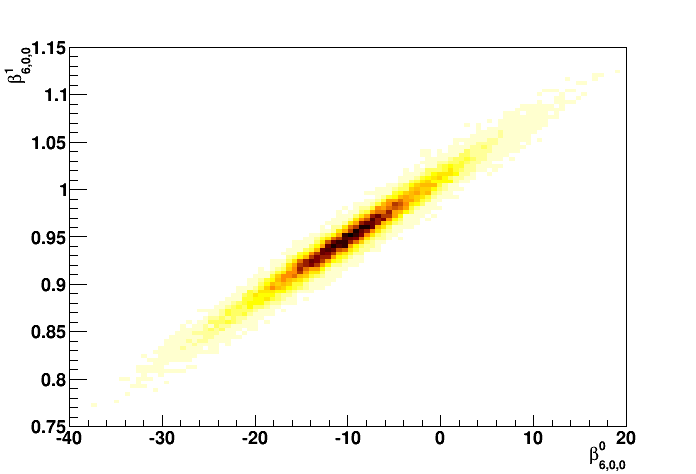
\includegraphics[width=0.5\textwidth]{corr_example}
    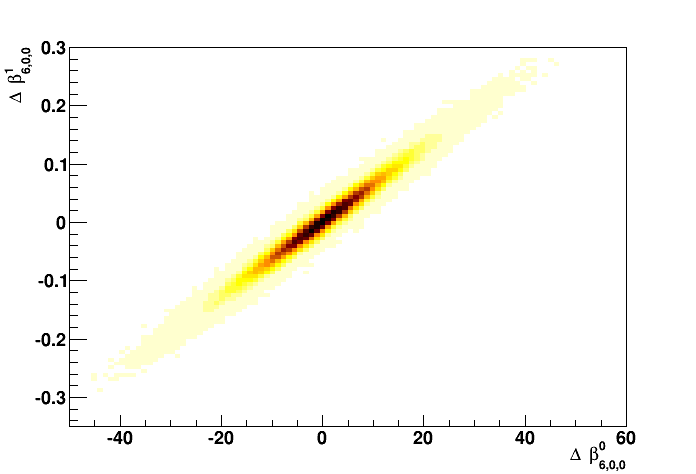
\includegraphics[width=0.5\textwidth]{diff_example}
  \end{center}
  \caption{Upper plot shows the histogram of the MCMC points for the
  multiplicative and additive parameters that affect the shape of the
  single-ring electron $e/\mu$ PID variable in Detector Region 6.  Note
  the strong correlations between the two parameters coming from the fact that
  the effects of varying these parameters partially cancel.  Lower plot shows
  the histogram of the accpeted parameter differences.  The DE-MCMC method
  draws from the lower distribution to better sample these correlated parameters.}
  \label{fig:parcor}
\end{figure}


\begin{figure}[h]
\begin{center}
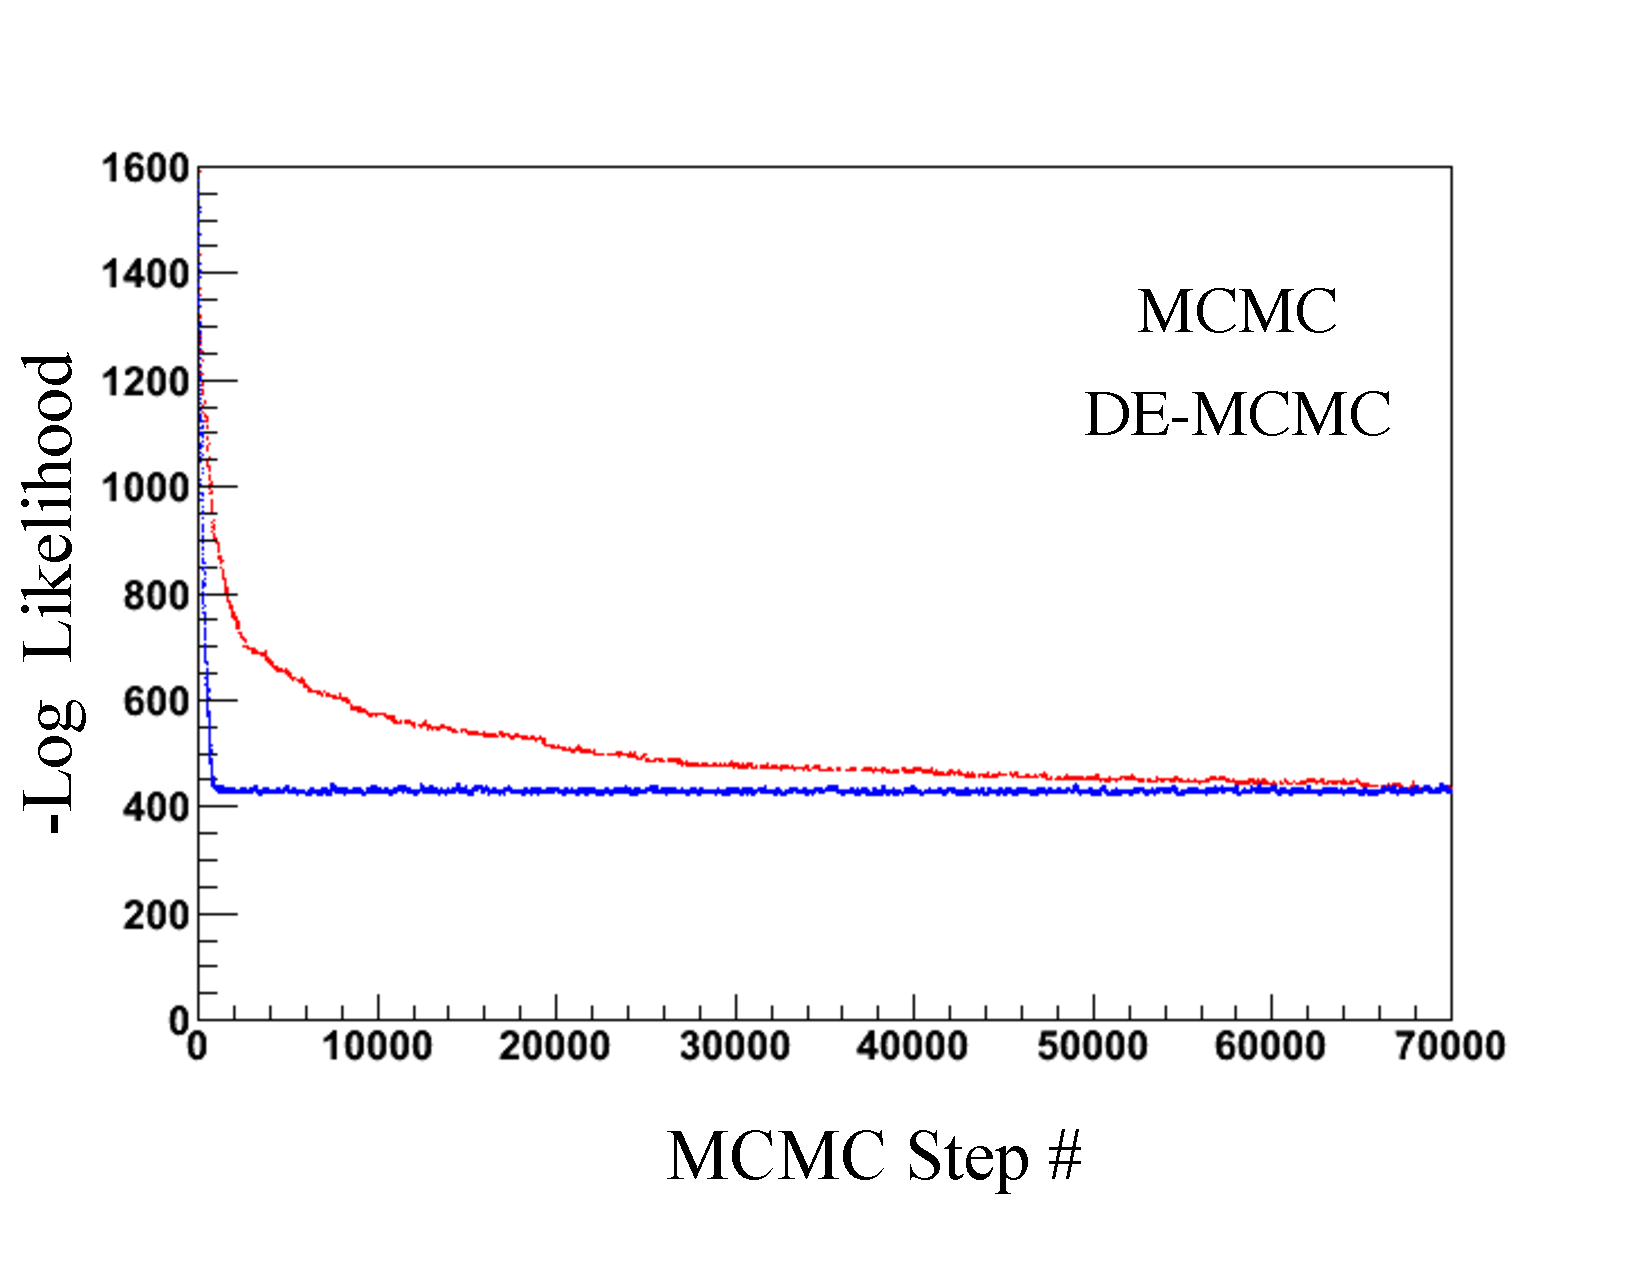
\includegraphics[width=0.5\textwidth]{plt_burnin}
\end{center}
\caption{Comparison of the burn-in period using an uncorrelated Gaussian
proposal fuction (red) and a proposal function that takes into account
parameter correlations using the DE-MCMC method (blue).  Both chains have been
tuned achieve an accpetance rate of $0.25\%$.  Both chains start at a the same
non-mimimal random starting point in the parameter space.}
\label{fig:burnin}
\end{figure}







\FloatBarrier


%-----------------------------------------------------------------------------


\section{Atmospheric Neutrino Fit Results}
\label{sec:fitresults}

Following the approach outlined in the previous section, we fit all 288
parameters for the atmospheric flux, cross section, and detector systematics to
the atmospheric data by running a sequence of Markov chains.  An initial MCMC is
performed with approximately two million steps to build up the distributions of
the differential parameters.  We then draw from these distributions when running
an additional two million steps of DE-MCMC\@.  The final output of this fit is 
a sampling of the (correlated) fit parameters that best agree with data. The parameter
correlations are visualized in Figure~\ref{fig:fitcorr}.

\begin{figure}[h]
  \begin{center}
    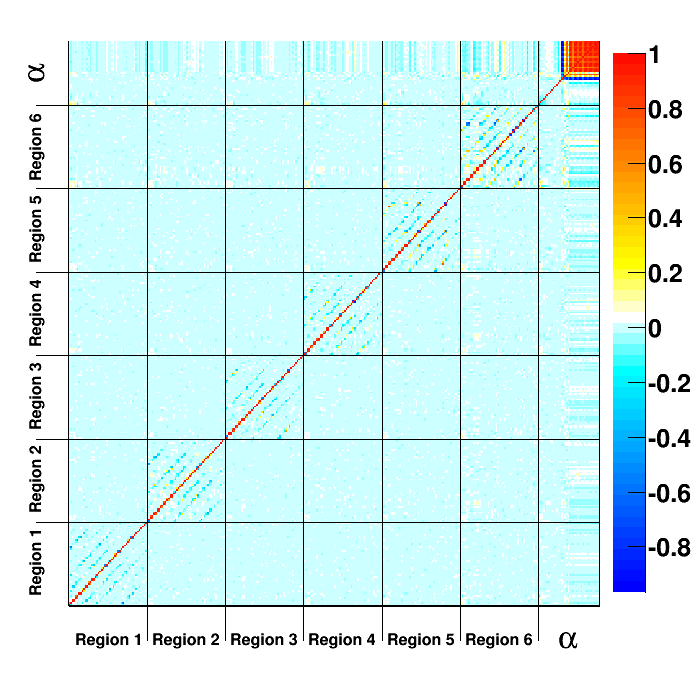
\includegraphics[width=0.7\textwidth]{hcorr_full_labeled}
  \end{center}
  \caption{Correlation matrix for all 288 parameters in the atmospheric fit.
  The labeled regions correspond to the SK detector regions defined in
  Section~\ref{subsec:DR}.  The region labeled $\alpha$ contains all of the
  flux, cross section, and normalization parameters.}
  \label{fig:fitcorr}
\end{figure}

To analyze the fit results, we
sample points from the DE-MCMC result and apply them to the simulated
atmospheric data\@.  In each histogram bin, we can calculate the mean and
statistical variance of the fit result, which is used to calculate the
statistical error.  Ideally, the observed data should be consistent with the
post-fit MCMC mean within the statistical error.  We find the average deviation
from the post-fit mean in each bin to be $1.11\sigma$, where $\sigma$ denotes
the statistical error of that bin.  The detailed fit results for each of the
histograms compared between data and MC can be seen in Section~\ref{sec:fithistos}.



%%% ATTRIBUTE 0 %%%%%%%%%%%%%%%%%%%%%%%%%%%%%%%%%%%%%%%%%%%%%%%%%%%%%%%%%%%%%%%%%%%
%\begin{figure}[h]
%  \begin{center}
%    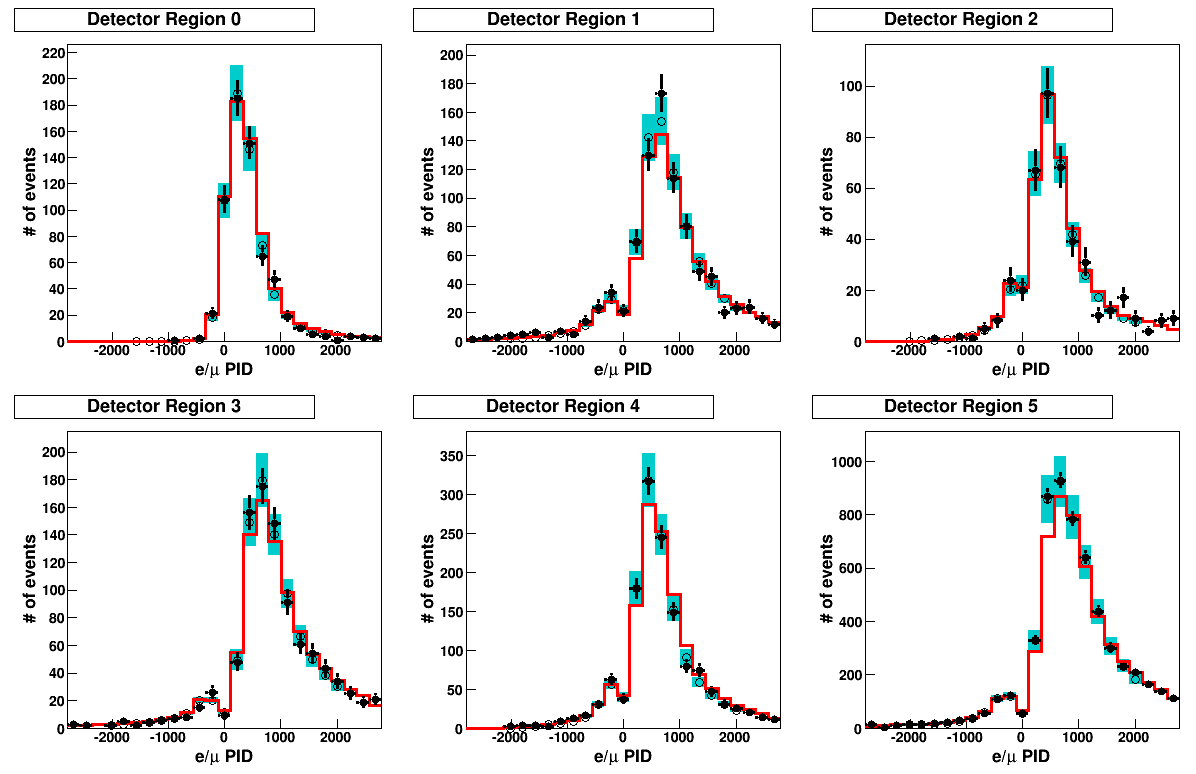
\includegraphics[width=0.9\textwidth]{demcmc_fitresult_samp0_attribute0} 
%  \end{center}
%  \caption{Fit results for the $l=0$ control sample (no decay electrons) for
%  the fiTQun $e/\mu$ PID variable in each of the detector regions.  Positive
%  values denote more $e$-like events, negative values denote more $\mu$-like
%  events.  Red histogram shows nominal MC prediction.  Black points represent
%  observed data.  Teal histogram shows post-fit distribution, where the mean is
%  the average of the DE-MCMC throws and the error bar is the square root of the
%  variance.}
%  \label{fig:fitresults_samp0_att0}
%\end{figure}
%
%
%\begin{figure}[h]
%  \begin{center}
%    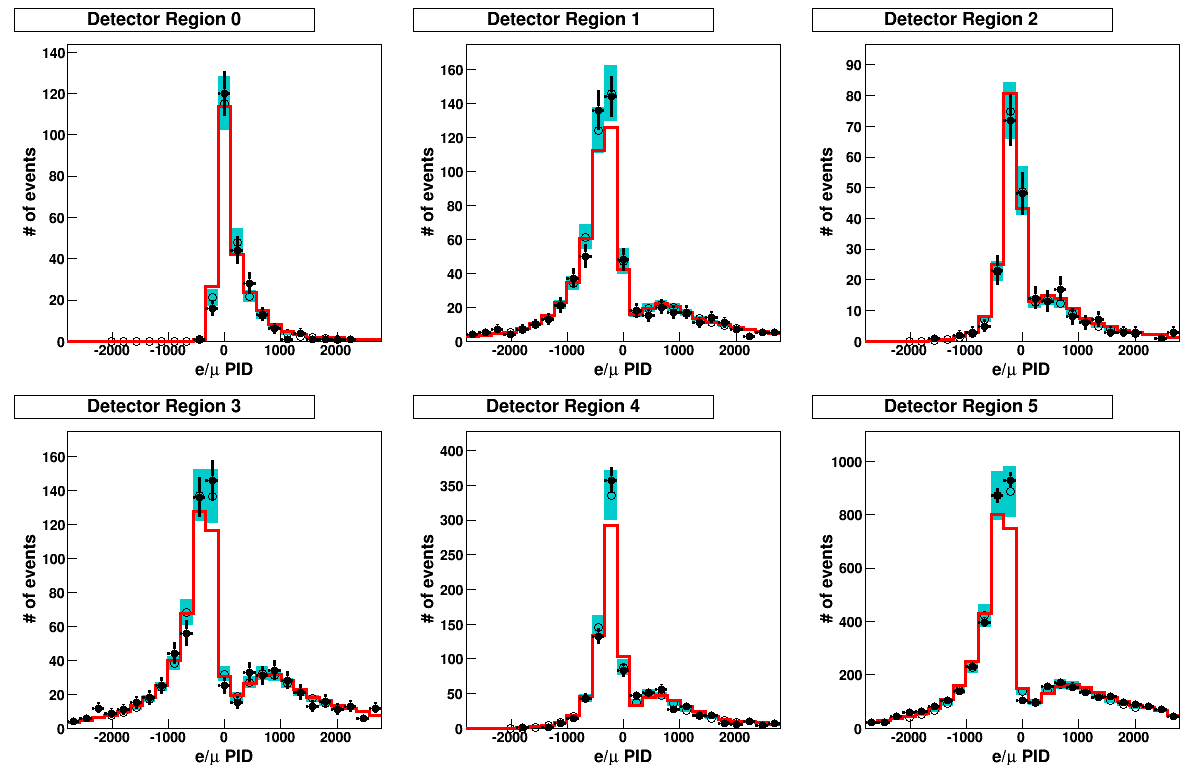
\includegraphics[width=0.9\textwidth]{demcmc_fitresult_samp1_attribute0} 
%  \end{center}
%  \caption{Fit results for the $l=1$ control sample (one decay electron) for
%  the fiTQun $e/\mu$ PID variable in each of the detector regions.  Positive
%  values denote more $e$-like events, negative values denote more $\mu$-like
%  events.  Red histogram shows nominal MC prediction.  Black points represent
%  observed data.  Teal histogram shows post-fit distribution, where the mean is
%  the average of the DE-MCMC throws and the error bar is the square root of the
%  variance.}
%  \label{fig:fitresults_samp1_att0}
%\end{figure}
%
%
%\begin{figure}[h]
%  \begin{center}
%    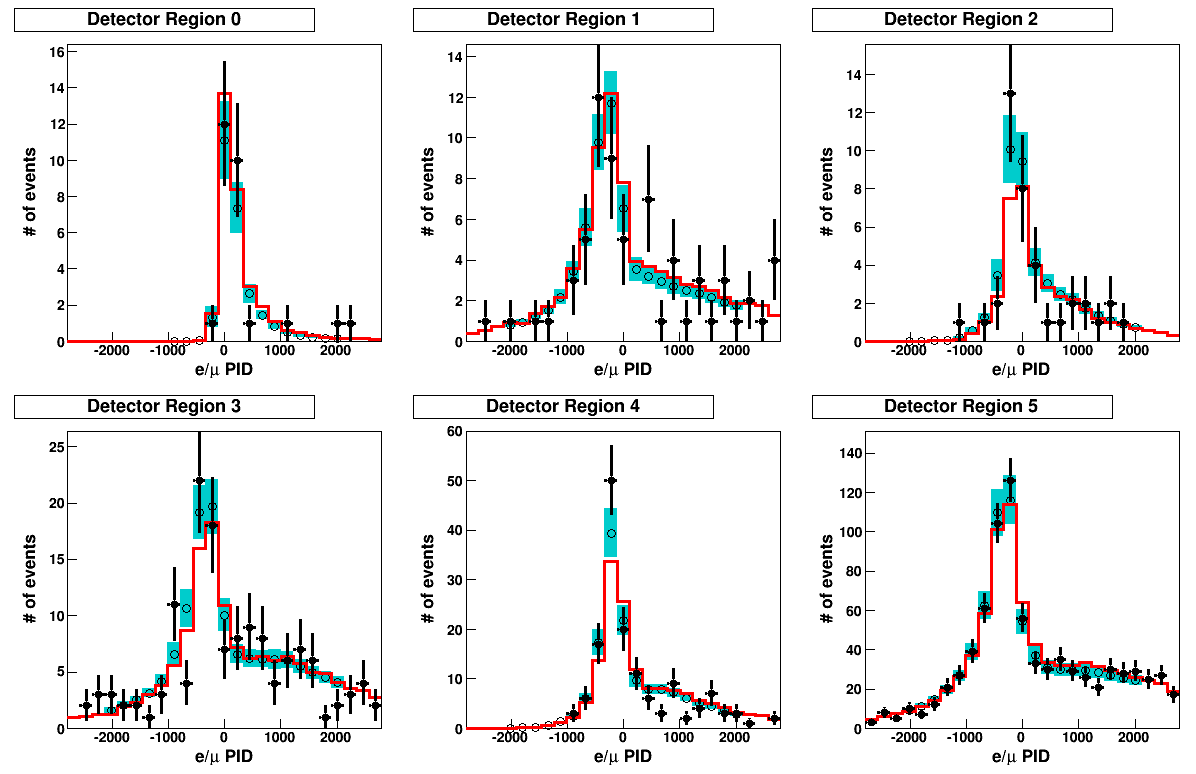
\includegraphics[width=0.9\textwidth]{demcmc_fitresult_samp2_attribute0} 
%  \end{center}
%  \caption{Fit results for the $l=2$ control sample (more than one decay
%  electron) for the fiTQun $e/\mu$ PID variable in each of the detector
%  regions.  Positive values denote more $e$-like events, negative values denote
%  more $\mu$-like events. Red histogram shows nominal MC prediction.  Black
%  points represent observed data.  Teal histogram shows post-fit distribution,
%  where the mean is the average of the DE-MCMC throws and the error bar is the
%  square root of the variance.}
%  \label{fig:fitresults_samp2_att0}
%\end{figure}
%
%
%%% ATTRIBUTE 1 %%%%%%%%%%%%%%%%%%%%%%%%%%%%%%%%%%%%%%%%%%%%%%%%%%%%%%%%%%%%%%%%%%%
%\begin{figure}[h]
%  \begin{center}
%    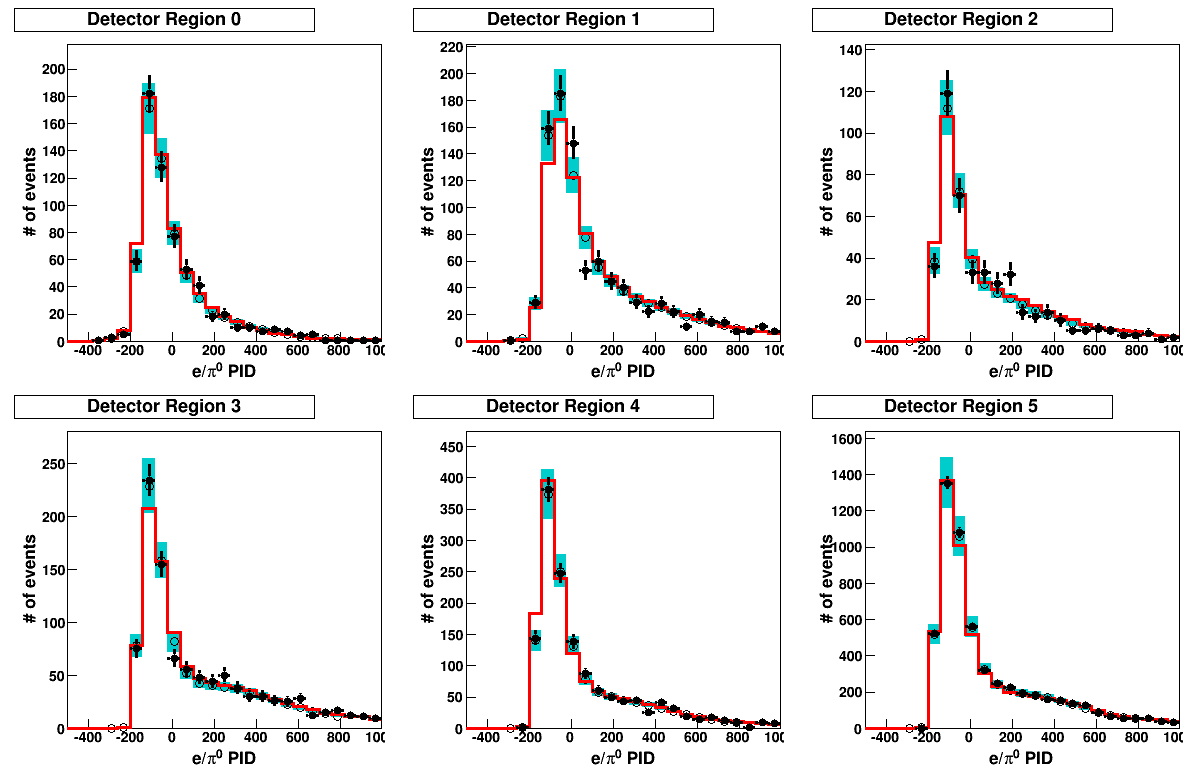
\includegraphics[width=0.9\textwidth]{demcmc_fitresult_samp0_attribute1} 
%  \end{center}
%  \caption{Fit results for the $l=0$ control sample (no decay electrons) for
%  the fiTQun $e/\pi^{0}$ PID variable in each of the detector regions. Positive
%  values denote more $\pi^{0}$-like events, negative values denote more
%  $e$-like events. Red histogram shows nominal MC prediction.  Black points
%  represent observed data.  Teal histogram shows post-fit distribution, where
%  the mean is the average of the DE-MCMC throws and the error bar is the square
%  root of the variance.}
%  \label{fig:fitresults_samp0_att1}
%\end{figure}
%
%
%\begin{figure}[h]
%  \begin{center}
%    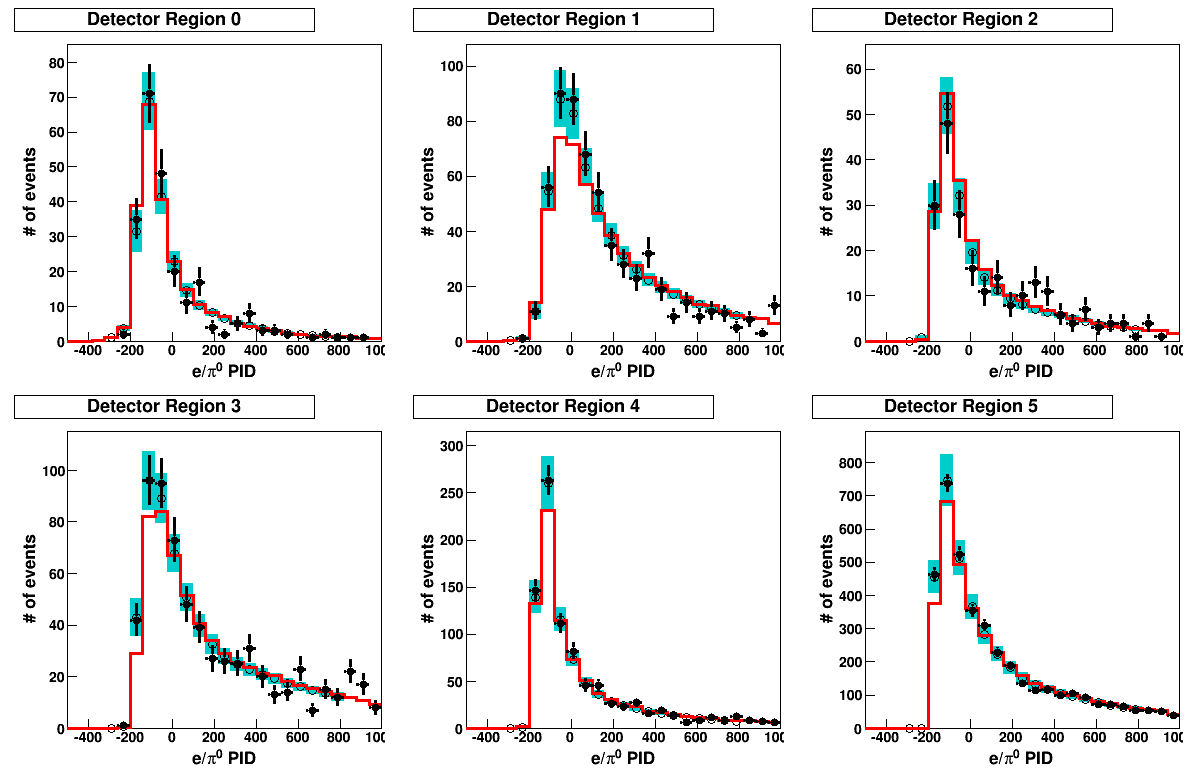
\includegraphics[width=0.9\textwidth]{demcmc_fitresult_samp1_attribute1} 
%  \end{center}
%  \caption{Fit results for the $l=1$ control sample (one decay electron) for
%  the fiTQun $e/\pi^{0}$ PID variable in each of the detector regions. Positive
%  values denote more $\pi^{0}$-like events, negative values denote more
%  $e$-like events. Red histogram shows nominal MC prediction.  Black points
%  represent observed data.  Teal histogram shows post-fit distribution, where
%  the mean is the average of the DE-MCMC throws and the error bar is the square
%  root of the variance.}
%  \label{fig:fitresults_samp1_att1}
%\end{figure}
%
%
%\begin{figure}[h]
%  \begin{center}
%    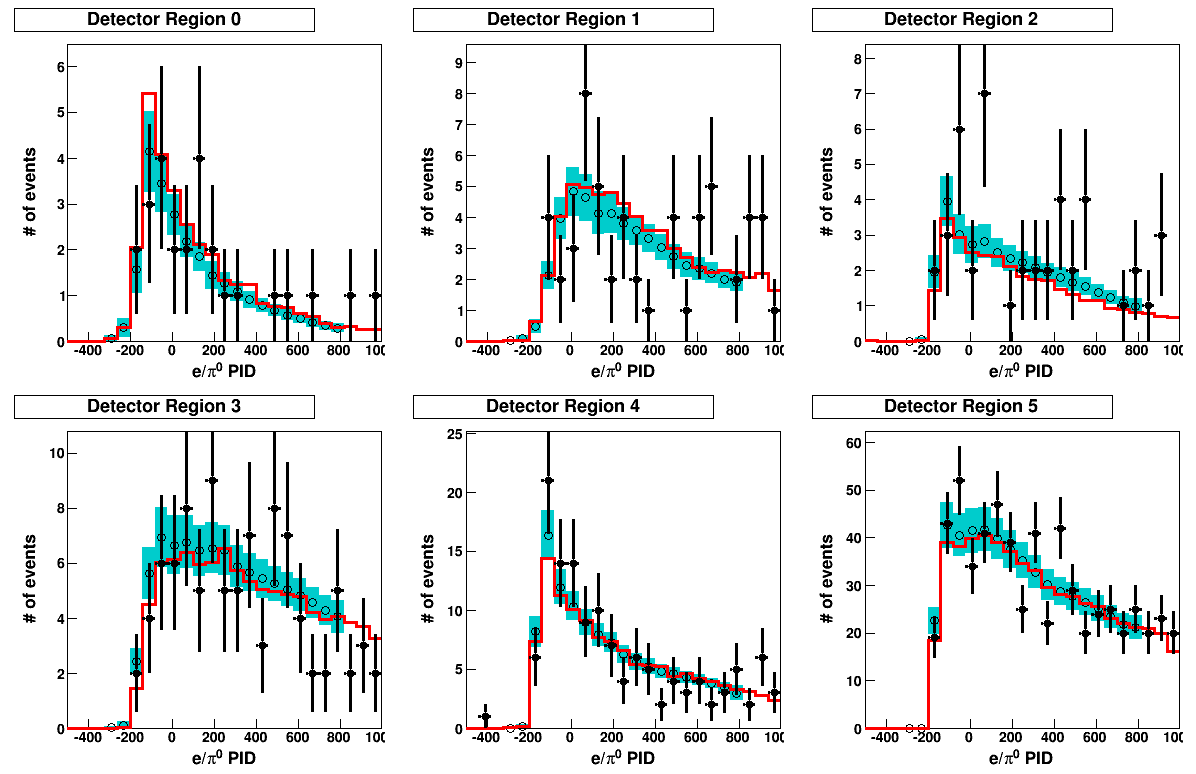
\includegraphics[width=0.9\textwidth]{demcmc_fitresult_samp2_attribute1} 
%  \end{center}
%  \caption{Fit results for the $l=2$ control sample (more than one decay
%  electron) for the fiTQun $e/\pi^{0}$ PID variable in each of the detector
%  regions.  Positive values denote more $\pi^{0}$-like events, negative values
%  denote more $e$-like events. Red histogram shows nominal MC prediction.
%  Black points represent observed data.  Teal histogram shows post-fit
%  distribution, where the mean is the average of the DE-MCMC throws and the
%  error bar is the square root of the variance.}
%  \label{fig:fitresults_samp2_att1}
%\end{figure}
%
%
%%% ATTRIBUTE 2 %%%%%%%%%%%%%%%%%%%%%%%%%%%%%%%%%%%%%%%%%%%%%%%%%%%%%%%%%%%%%%%%%%%
%\begin{figure}[h]
%  \begin{center}
%    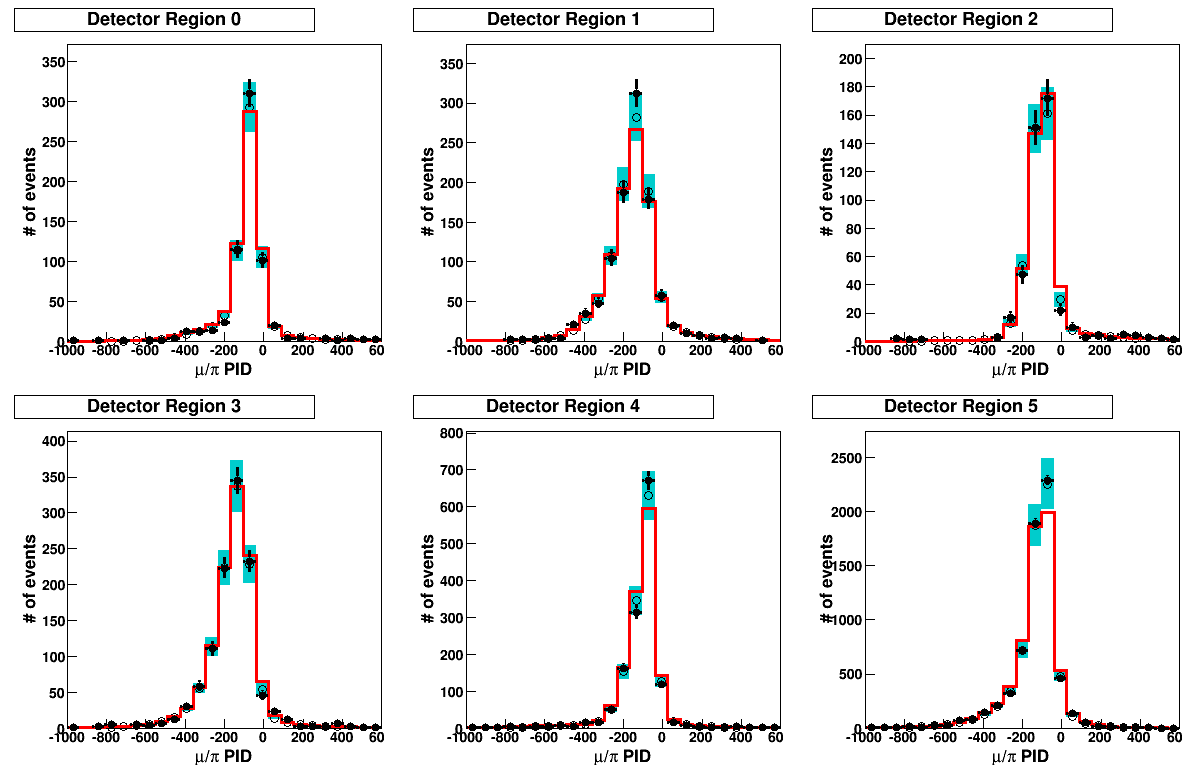
\includegraphics[width=0.9\textwidth]{demcmc_fitresult_samp0_attribute2} 
%  \end{center}
%  \caption{Fit results for the $l=0$ control sample (no decay electrons) for
%  the fiTQun $\mu/\pi$ PID variable in each of the detector regions. Positive
%  values denote more $\pi$-like events, negative values denote more $\mu$-like
%  events. Red histogram shows nominal MC prediction.  Black points represent
%  observed data.  Teal histogram shows post-fit distribution, where the mean is
%  the average of the DE-MCMC throws and the error bar is the square root of the
%  variance.}
%  \label{fig:fitresults_samp0_att2}
%\end{figure}
%
%
%\begin{figure}[h]
%  \begin{center}
%    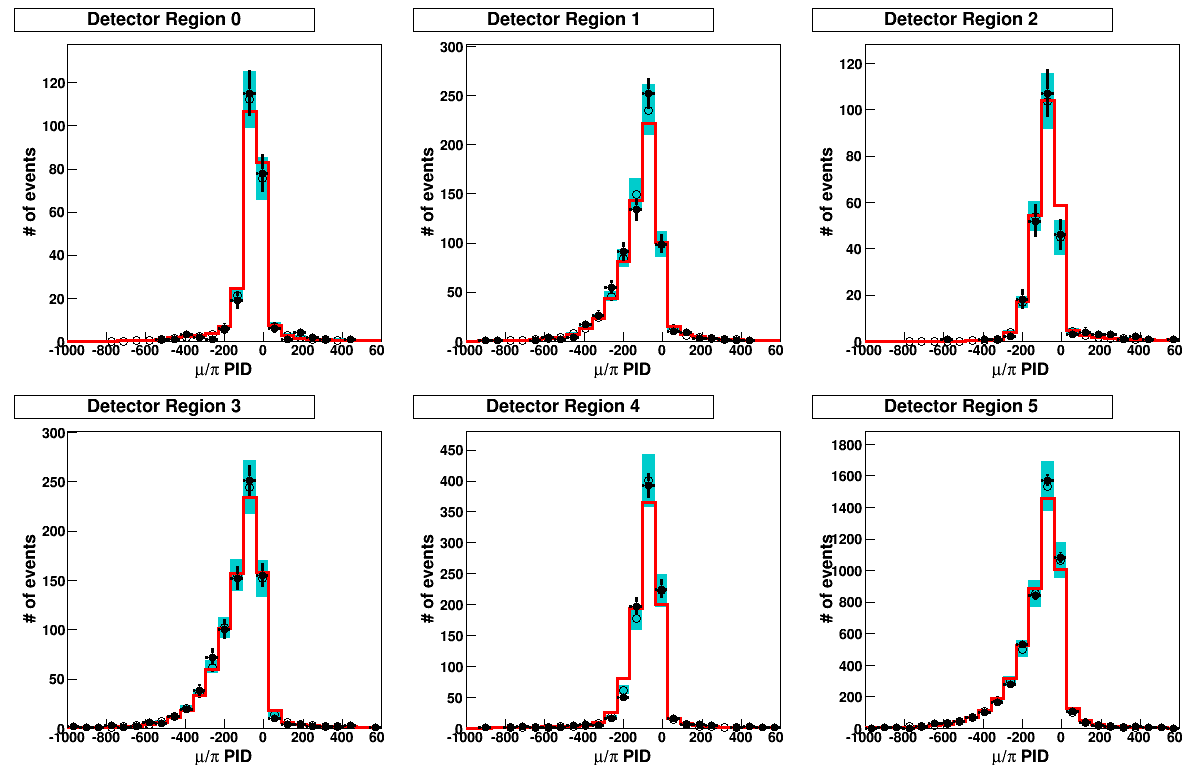
\includegraphics[width=0.9\textwidth]{demcmc_fitresult_samp1_attribute2} 
%  \end{center}
%  \caption{Fit results for the $l=1$ control sample (one decay electron) for
%  the fiTQun $\mu/\pi$ PID variable in each of the detector regions.  Positive
%  values denote more $\pi$-like events, negative values denote more $\mu$-like
%  events. Red histogram shows nominal MC prediction.  Black points represent
%  observed data.  Teal histogram shows post-fit distribution, where the mean is
%  the average of the DE-MCMC throws and the error bar is the square root of the
%  variance.} 
%  \label{fig:fitresults_samp1_att2}
%\end{figure}
%
%
%\begin{figure}[h]
%  \begin{center}
%    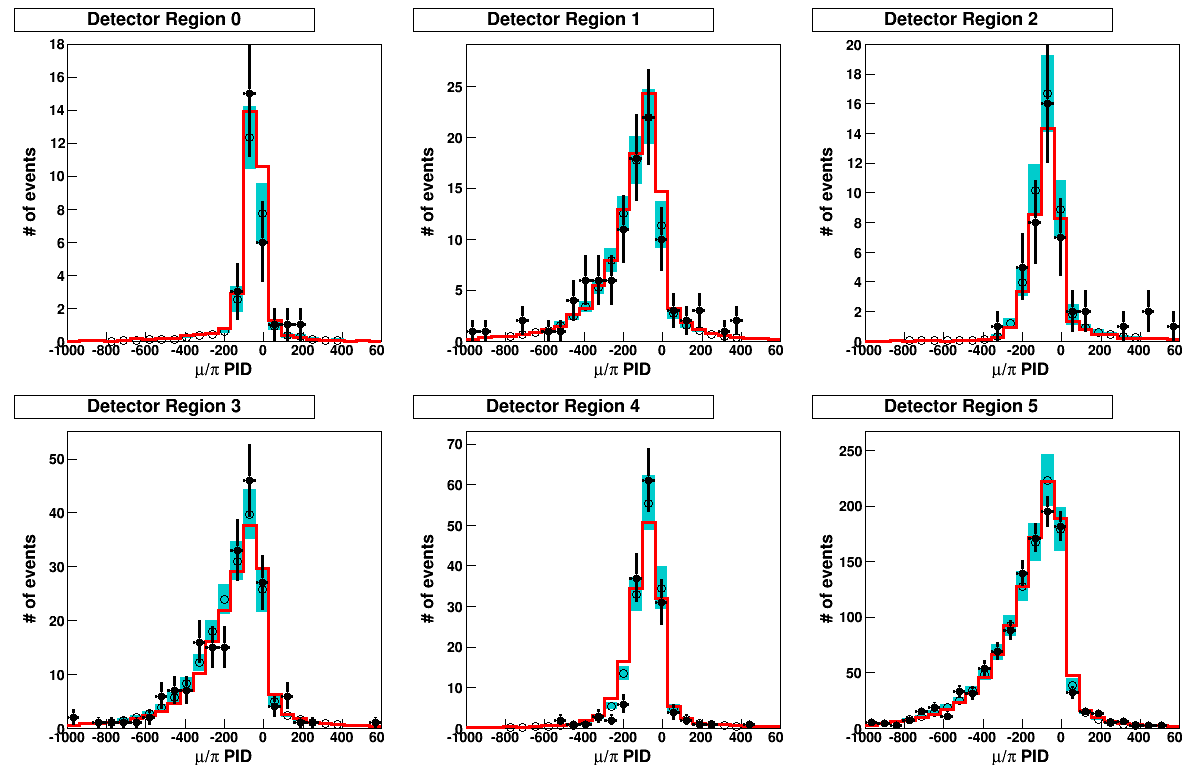
\includegraphics[width=0.9\textwidth]{demcmc_fitresult_samp2_attribute2} 
%  \end{center}
%  \caption{Fit results for the $l=2$ control sample (more than one decay
%  electron) for the fiTQun $\mu/\pi$ PID variable in each of the detector
%  regions.  Positive values denote more $\pi$-like events, negative values
%  denote more $\mu$-like events. Red histogram shows nominal MC prediction.
%  Black points represent observed data.  Teal histogram shows post-fit
%  distribution, where the mean is the average of the DE-MCMC throws and the
%  error bar is the square root of the variance.}
%  \label{fig:fitresults_samp2_att2}
%\end{figure}
%
%
%%% ATTRIBUTE 3 %%%%%%%%%%%%%%%%%%%%%%%%%%%%%%%%%%%%%%%%%%%%%%%%%%%%%%%%%%%%%%%%%%%
%\begin{figure}[h]
%  \begin{center}
%    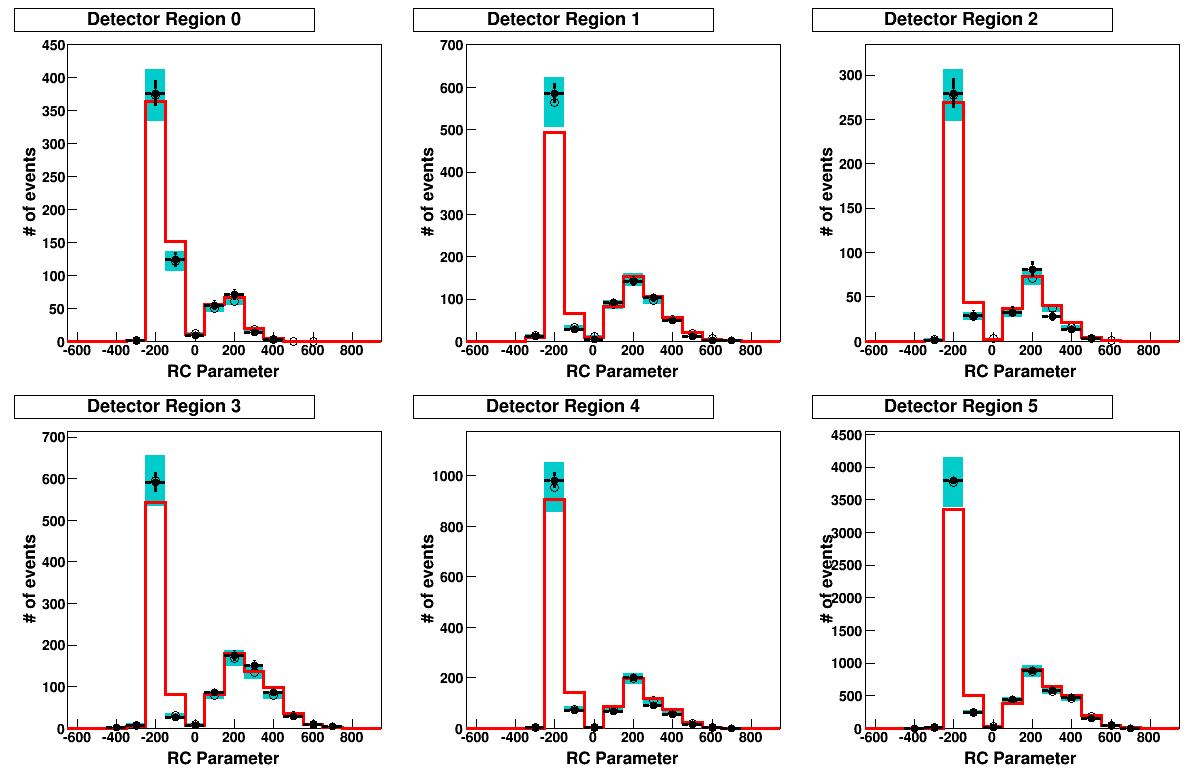
\includegraphics[width=0.9\textwidth]{demcmc_fitresult_samp0_attribute3} 
%  \end{center}
%  \caption{Fit results for the $l=0$ control sample (no decay electrons) for
%  the fiTQun RC (ring-counting) variable in each of the detector regions.
%  Positive values denote more multi-ring-like events, negative values denote
%  more single-ring-like events. Red histogram shows nominal MC prediction.
%  Black points represent observed data.  Teal histogram shows post-fit
%  distribution, where the mean is the average of the DE-MCMC throws and the
%  error bar is the square root of the variance.}
%  \label{fig:fitresults_samp0_att3}
%\end{figure}
%
%
%\begin{figure}[h]
%  \begin{center}
%    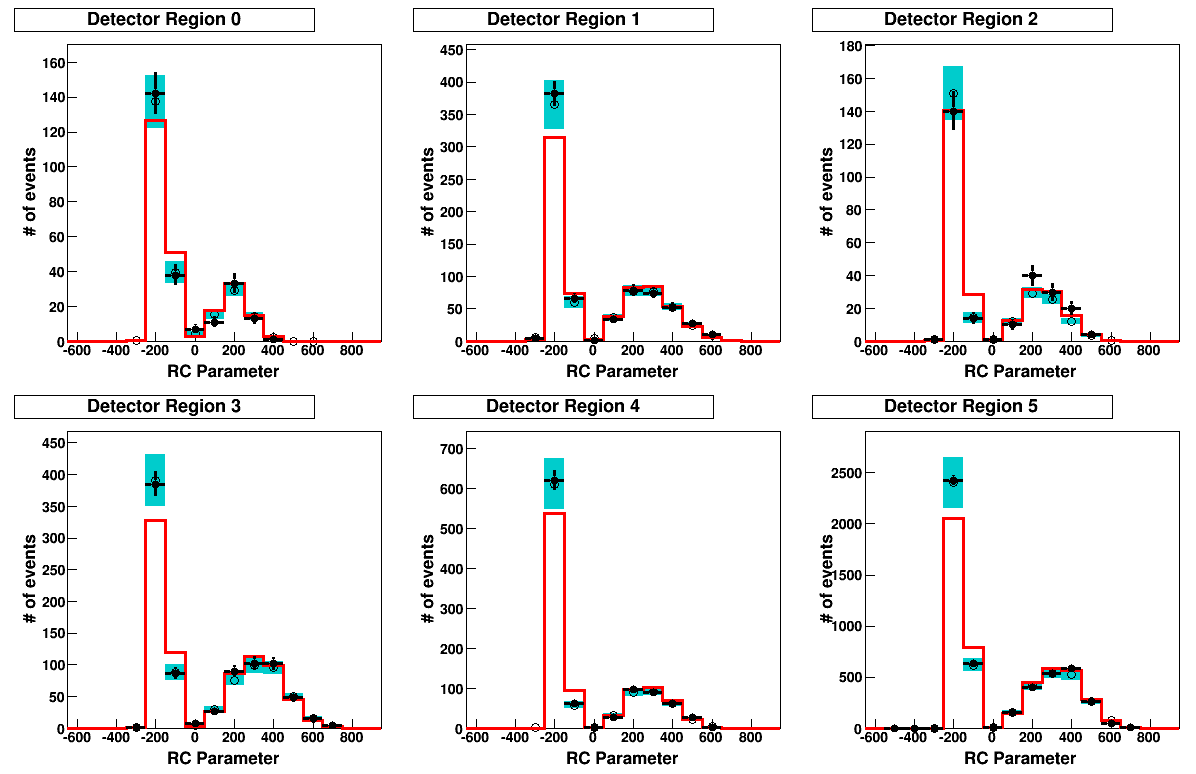
\includegraphics[width=0.9\textwidth]{demcmc_fitresult_samp1_attribute3} 
%  \end{center}
%  \caption{Fit results for the $l=1$ control sample (one decay electron) for
%  the fiTQun $\mu/\pi$ PID variable in each of the detector regions.  Positive
%  values denote more multi-ring-like events, negative values denote more
%  single-ring-like events. Red histogram shows nominal MC prediction.  Black
%  points represent observed data.  Teal histogram shows post-fit distribution,
%  where the mean is the average of the DE-MCMC throws and the error bar is the
%  square root of the variance.}
%  \label{fig:fitresults_samp1_att3}
%\end{figure}
%
%
%\begin{figure}[h]
%  \begin{center}
%    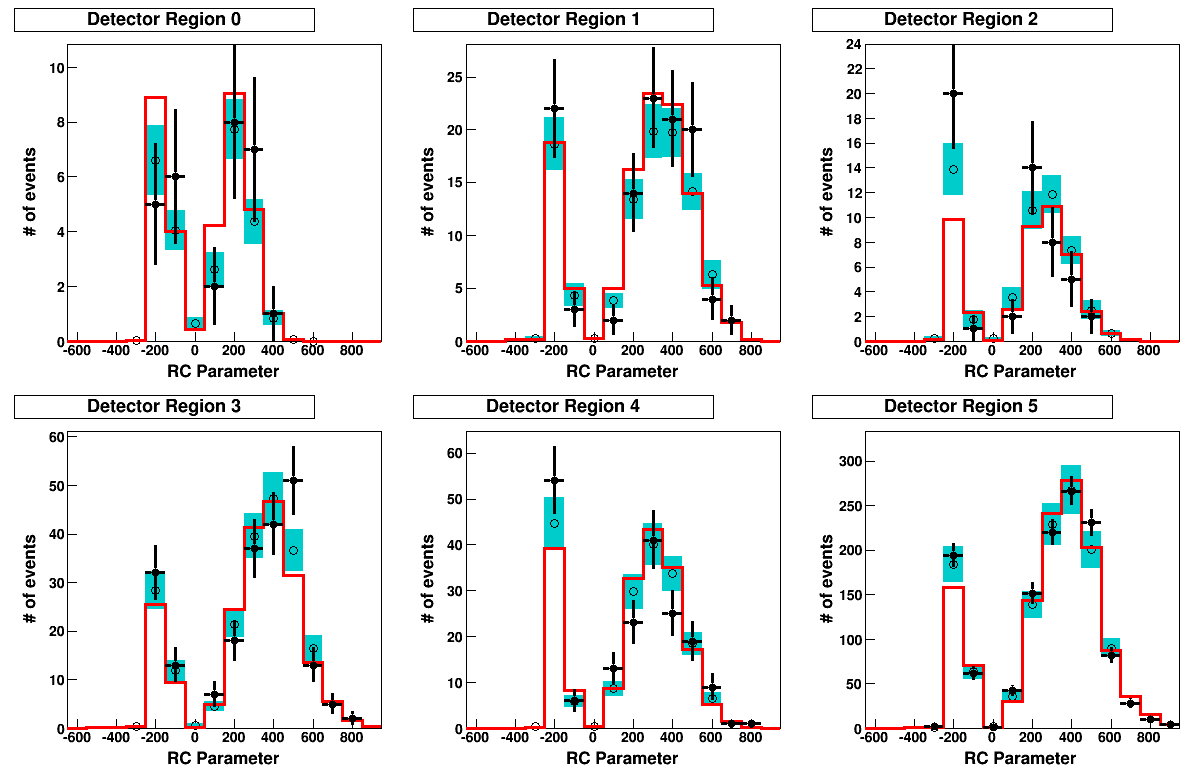
\includegraphics[width=0.9\textwidth]{demcmc_fitresult_samp2_attribute3} 
%  \end{center}
%  \caption{Fit results for the $l=2$ control sample (more than one decay
%  electron) for the fiTQun $\mu/\pi$ PID variable in each of the detector
%  regions.  Positive values denote more multi-ring-like events, negative values
%  denote more single-ring-like events.  Red histogram shows nominal MC
%  prediction.  Black points represent observed data.  Teal histogram shows
%  post-fit distribution, where the mean is the average of the DE-MCMC throws
%  and the error bar is the square root of the variance.}
%  \label{fig:fitresults_samp2_att3}
%\end{figure}
%
%
%
%\begin{figure}[h]
%  \begin{center}
%   \centering
%   \begin{tabular}[h]{l l}
%    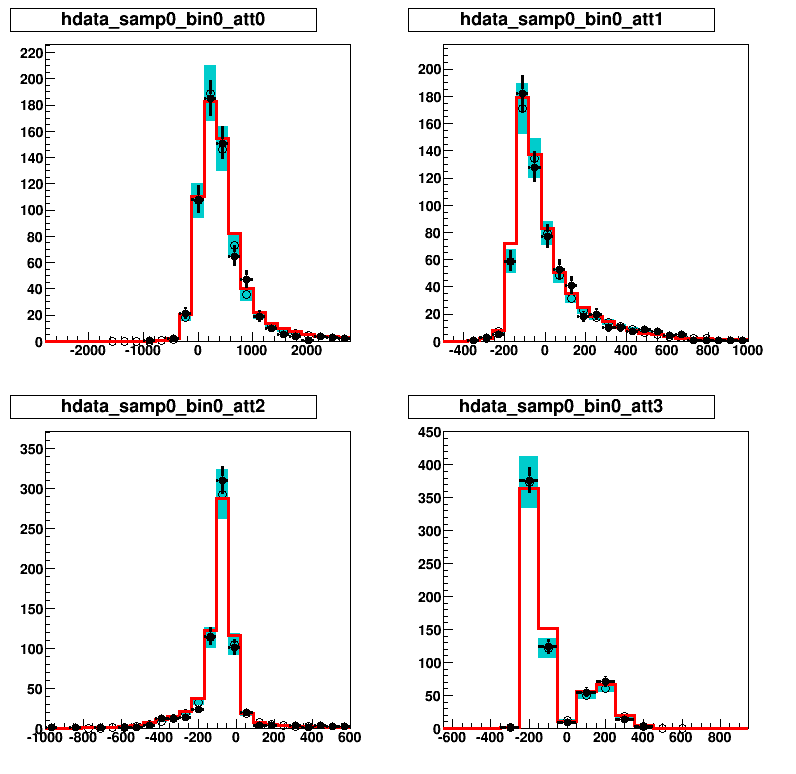
\includegraphics[width=0.55\textwidth]{demcmc_fitresult_samp0_bin0} 
%     &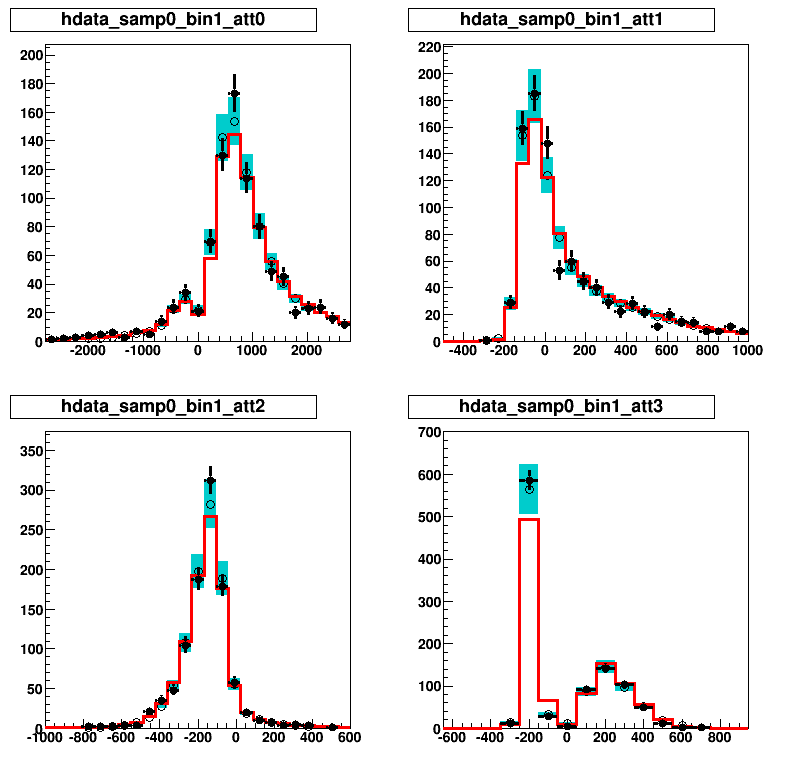
\includegraphics[width=0.55\textwidth]{demcmc_fitresult_samp0_bin1} \\
%     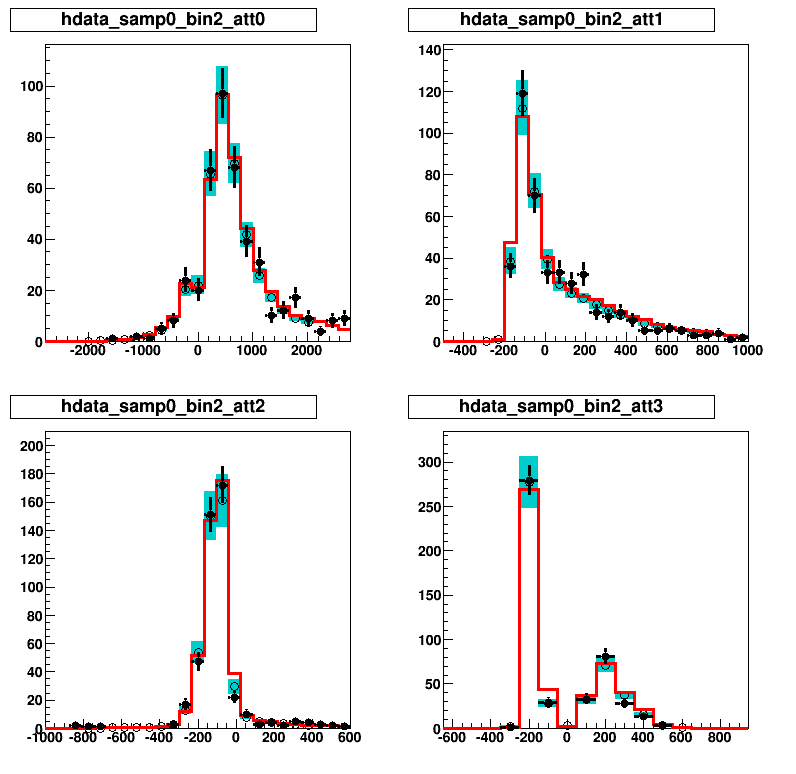
\includegraphics[width=0.55\textwidth]{demcmc_fitresult_samp0_bin2}   
%     &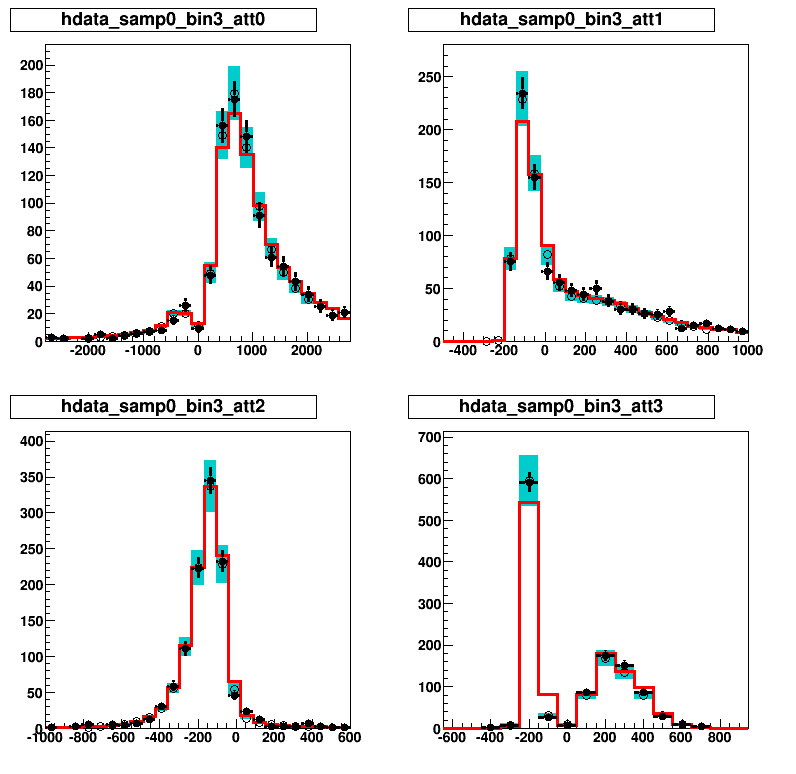
\includegraphics[width=0.55\textwidth]{demcmc_fitresult_samp0_bin3} \\ 
%     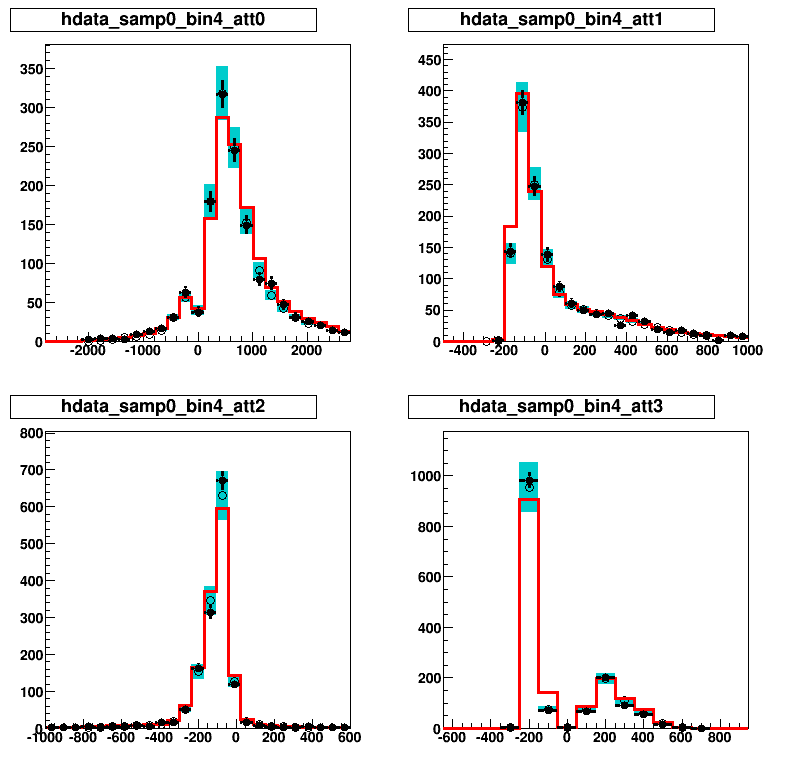
\includegraphics[width=0.55\textwidth]{demcmc_fitresult_samp0_bin4} 
%     &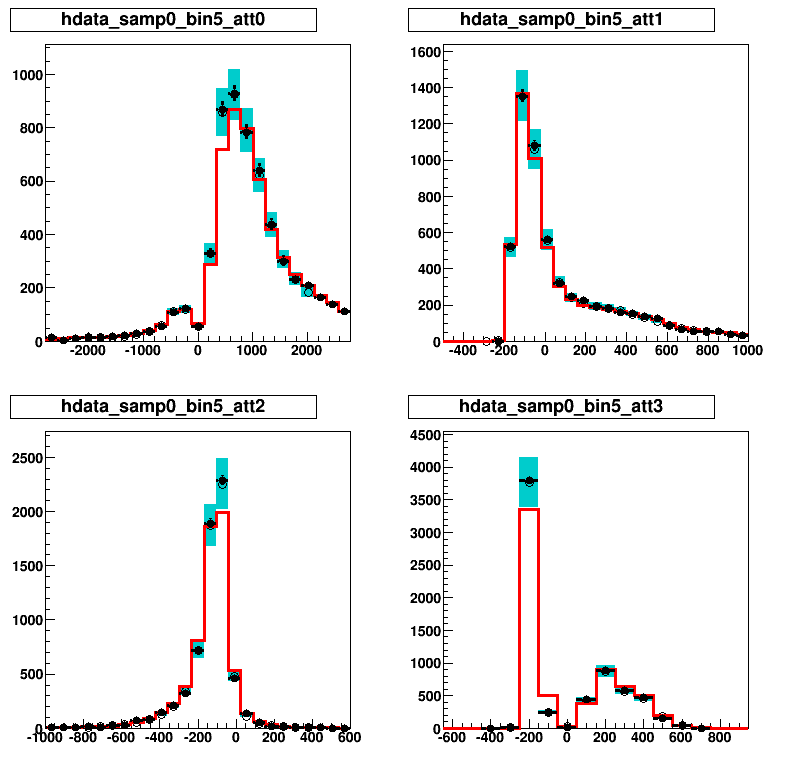
\includegraphics[width=0.55\textwidth]{demcmc_fitresult_samp0_bin5} 
%  \end{tabular}
%  \end{center}
%  \caption{Fit results for the $l=0$ control sample (no decay electrons) for each
%  fiTQun cut variable in each of the detector regions. Red histogram shows
%  nominal MC prediction.  Black points represent observed data.  Teal histogram
%  shows post-fit distribution, where the mean is the average of the DE-MCMC
%  throws and the error bar is the square root of the variance.}
%  \label{fig:fitresults_samp0}
%\end{figure}
%
%
%\begin{figure}[h]
%  \begin{center}
%   \begin{tabular}[h]{c c c}
%     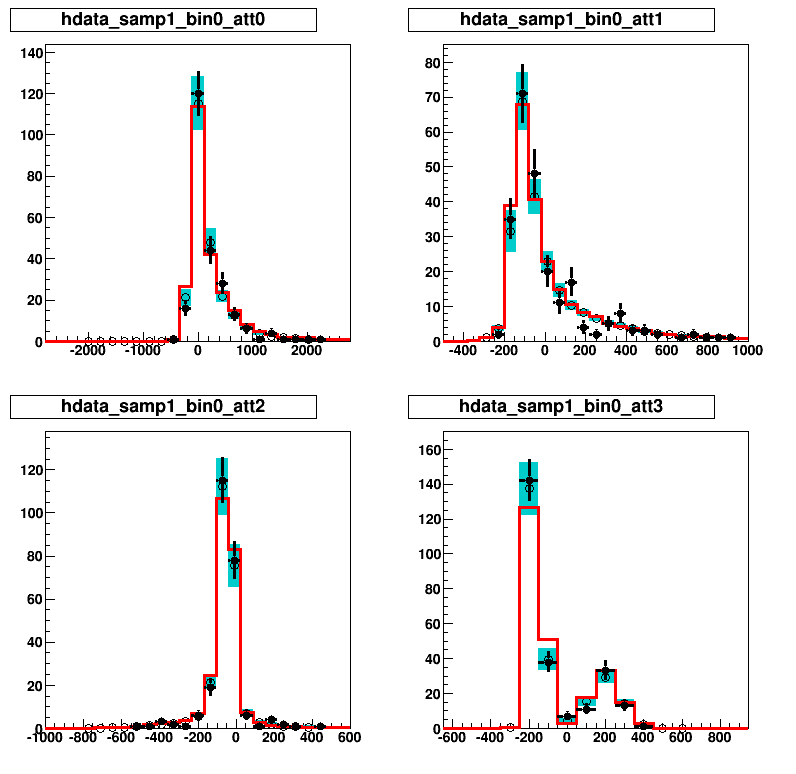
\includegraphics[width=0.33\textwidth]{demcmc_fitresult_samp1_bin0} 
%      &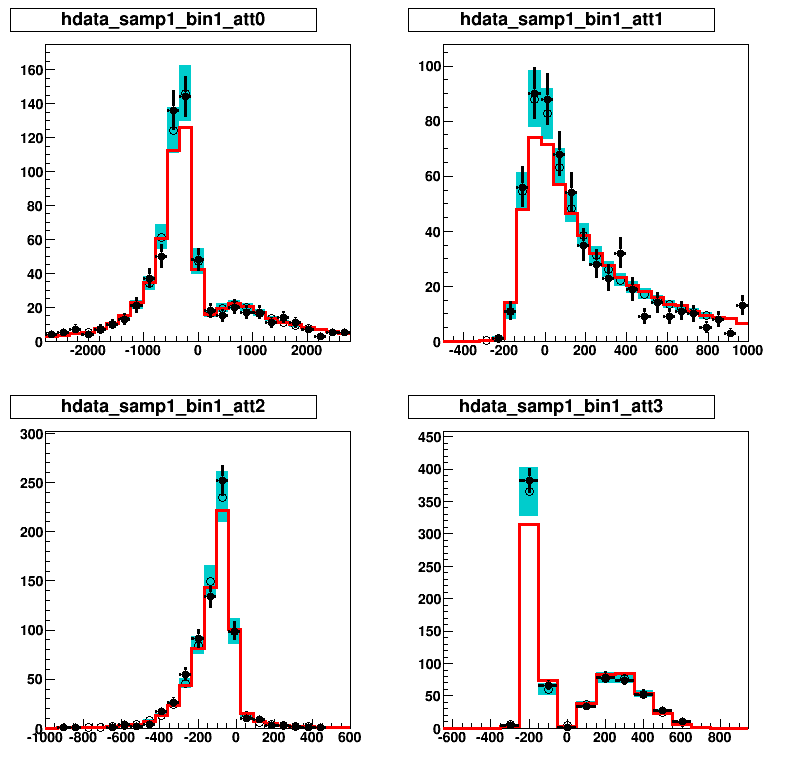
\includegraphics[width=0.33\textwidth]{demcmc_fitresult_samp1_bin1} 
%      &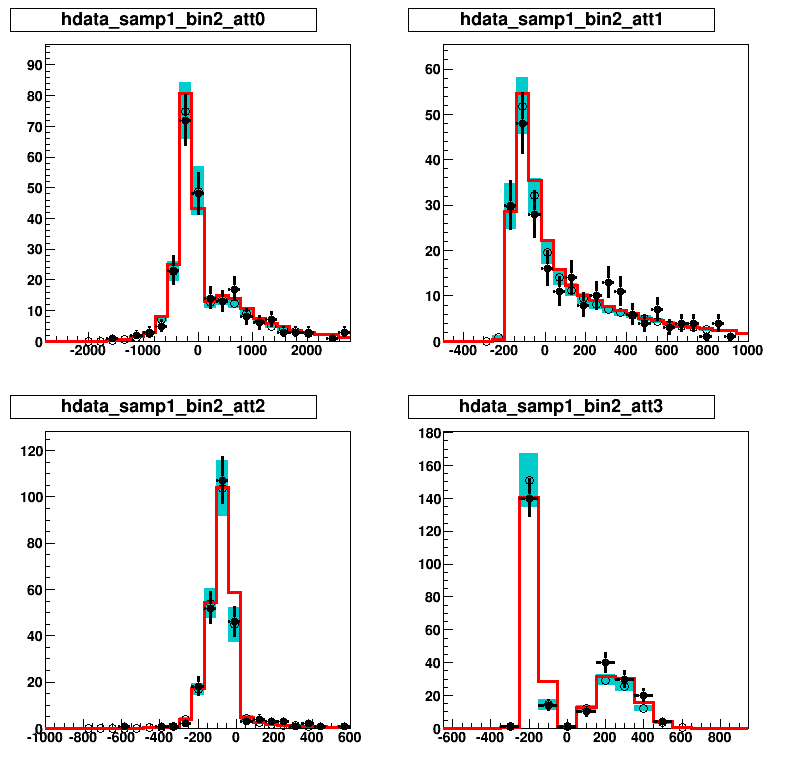
\includegraphics[width=0.33\textwidth]{demcmc_fitresult_samp1_bin2}  \\ 
%      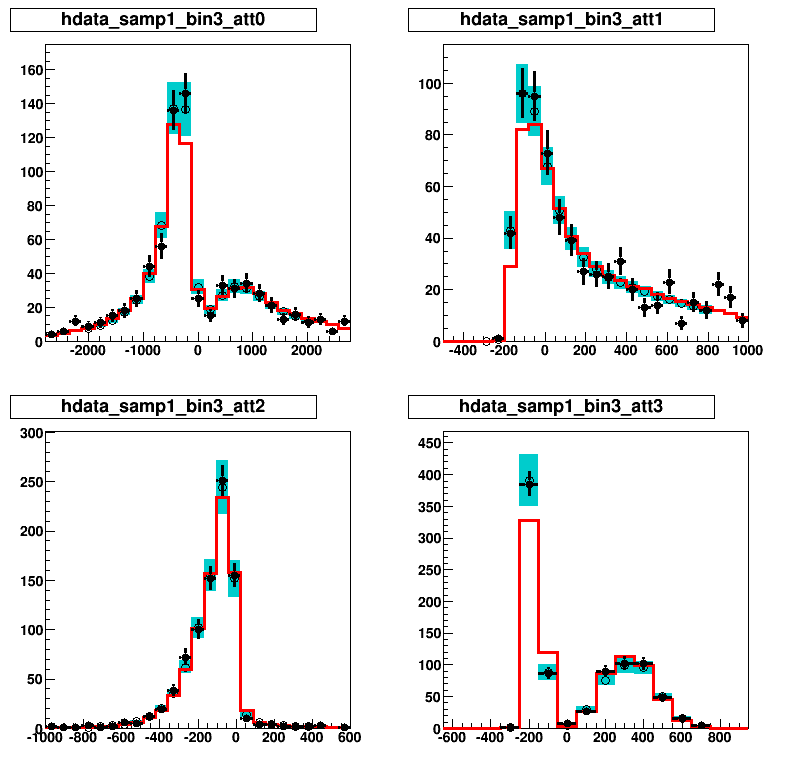
\includegraphics[width=0.33\textwidth]{demcmc_fitresult_samp1_bin3} 
%      &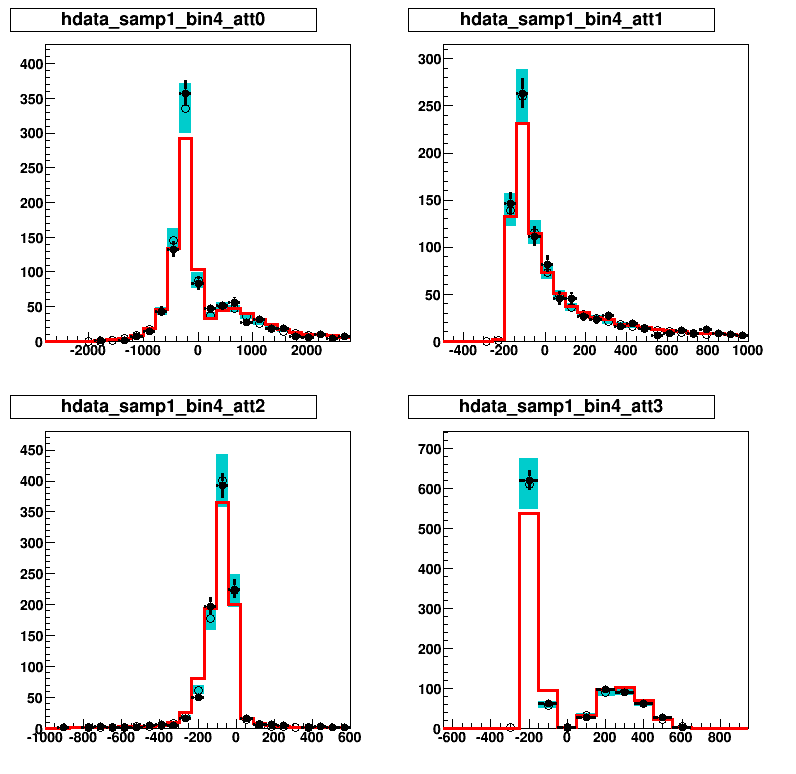
\includegraphics[width=0.33\textwidth]{demcmc_fitresult_samp1_bin4} 
%      &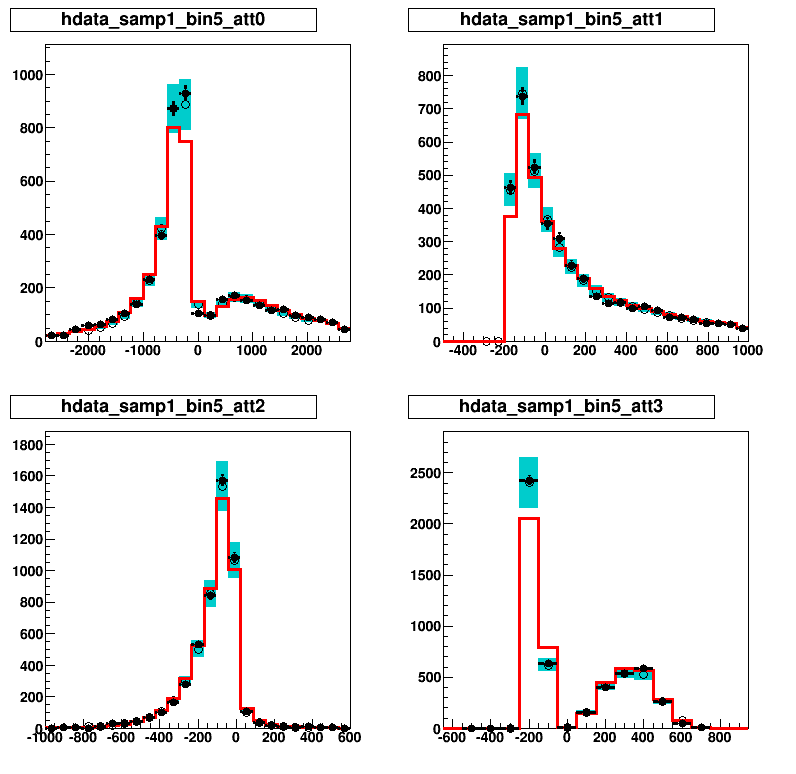
\includegraphics[width=0.33\textwidth]{demcmc_fitresult_samp1_bin5} 
%  \end{tabular}
%  \end{center}
%  \caption{Fit results for the $l = 1$ control sample (one decay electron) for each
%  fiTQun cut variable in each of the detector regions. Red histogram shows
%  nominal MC prediction.  Black points represent observed data.  Teal histogram
%  shows post-fit distribution, where the mean is the average of the DE-MCMC
%  throws and the error bar is the square root of the variance.}
%  \label{fig:fitresults_samp1}
%\end{figure}
%
%
%\begin{figure}[h]
%  \begin{center}
%   \begin{tabular}[h]{c c c}
%     \includegraphics[width=0.33\textwidth]{demcmc_fitresult_samp2_bin0} 
%      &\includegraphics[width=0.33\textwidth]{demcmc_fitresult_samp2_bin1} 
%      &\includegraphics[width=0.33\textwidth]{demcmc_fitresult_samp2_bin2}  \\ 
%      \includegraphics[width=0.33\textwidth]{demcmc_fitresult_samp2_bin3} 
%      &\includegraphics[width=0.33\textwidth]{demcmc_fitresult_samp2_bin4} 
%      &\includegraphics[width=0.33\textwidth]{demcmc_fitresult_samp2_bin5} 
%  \end{tabular}
%  \end{center}
%  \caption{Fit results for the $l = 2$ control sample (more than one decay electron) for each
%  fiTQun cut variable in each of the detector regions. Red histogram shows
%  nominal MC prediction.  Black points represent observed data.  Teal histogram
%  shows post-fit distribution, where the mean is the average of the DE-MCMC
%  throws and the error bar is the square root of the variance.}
%  \label{fig:fitresults_samp2}
%\end{figure}

%-----------------------------------------------------------------------------

\FloatBarrier


%-----------------------------------------------------------------------------

%-----------------------------------------------------------------------------
% FV Optimization
%-----------------------------------------------------------------------------
\section{Optimization of fiTQun Fiducial Volume Cuts}
\label{sec:fvopt}


%-----------------------------------------------------------------------------
% Intro
%-----------------------------------------------------------------------------
\subsection{Introduction}
\label{subsec:fvintro}


Since the fiTQun algorithm represents a fundamental change in the SK
reconstruction methods, a new set of optimization studies must be performed to
determine the best event selection cuts for the T2K oscillation analyses.
The optimization of the topological cuts that separate the T2K \numu and \nue
events are described in detail in TN-319~\cite{tn319}. In this section
we will describe a separate analysis for determining the fiducial volume (FV) cuts for each
T2K sample.  

The choice of FV cuts for the fiTQun T2K event selections presents a formidable
optimization problem. As the FV cuts are loosened, more neutrino events are
allowed into the T2K samples, which improves the statistical constraint on the
oscillation parameters.  However, accepting events from regions near the inner
detector (ID) wall may also introduce additional backgrounds that counteract
any statistical gain.  Further complicating the situation is the presence of
systematic uncertainties, which may be larger in regions near the ID wall and
also potentially offset any statistical gain in sensitivity.

The overall approach to this problem is to define a figure of merit that
approximates the sensitivity to the neutrino oscillation parameters in the
presence of the estimated systematics. The systematics in various detector
regions are then constrained use the results of the atmospheric neutrino fit
described in Section~\ref{sec:methods}.  The FV cuts for each T2K sample are 
then taken to be the cuts that maximize this figure of merit (subject to some
constraints). Each T2K selection faces a different set of backgrounds near the ID
wall, so the FV cuts for each sample are estimated separately.  The optimized cuts
are then applied to each selection for both FHC and RHC modes


%-----------------------------------------------------------------------------
% Figure of Merit
%-----------------------------------------------------------------------------
\subsection{Figure of Merit}
\label{subsec:metric}


The determination of the ``optimal'' fiducial volume cuts requires a
quantitative definition of ``optimal''.  Ideally, the quantity we would like to
optimize is the sensitivity to the underlying neutrino oscillation parameters,
(and indeed future optimization analyses should strive to do this), but the
precise determination of the sensitivity is itself a complex analyses that does
not lend itself well to repeated sampling under varying FV cut assumptions.
For this analysis, we choose instead to use a simple numerical figure of merit
as our optimization metric.  At minimum, the figure of merit should try to
account for the competing effects of statistics, purity and uncertainty. 

The FV optimization figure of merit can be derived by maximizing the
sensitivity for a very simplified parameter estimation framework. We
consider the likelihood of observing $X$ events in some Poisson process whose
mean depends on an underlying parameter $\theta$. Clearly, for the T2K
analysis, $X$ represents the observed number of neutrino events in some sample,
and $\theta$ represents the corresponding oscillation parameter of interest
(i.e. \thdis or \dcp).  If we expect $X>10$ we may approximate the probability
of observing $X$ given $\theta$ to be Gaussian, so the corresponding likelihood
is:
%
\begin{equation}
  -log[\mathcal{L}(X|\theta)] \approx \frac{(X - N(\theta))^{2}}{2\sigma^{2}}
\end{equation}
%
where $N(\theta)$ is the Poisson mean as a function of $\theta$, and $\sigma$
is some measure of the uncertainty associated in measuring $X$ that will be
quantified later. The sensitivity to the parameter  $\theta$ depends on the
curvature of the likelihood, which can be expressed as:
%
\begin{equation}
\label{eq:lderiv}
  -\frac{\partial^{2}  log[\mathcal{L}(X|\theta)]}{\partial \theta^{2}} =
  \frac{1}{\sigma^{2}}\bigg[(X - N)\frac{\partial^{2} N}{\partial \theta^{2}} - \bigg(\frac{\partial N}{\partial \theta}\bigg)^{2} \bigg]
\end{equation}
%
We assume the observed data $X$ is drawn from a Poisson distribution with a
mean $N(\theta_{true})$.  The expectation value of the curvature at the true
parameter value over an ensemble of hypothetical measurements can then be
expressed as:
%
\begin{equation}
  \bigg\langle \frac{\partial^{2} log[\mathcal{L}(X|\theta)]}{\partial \theta^{2}} \Big|_{\theta = \theta_{true}}  \bigg\rangle_{X} = 
  \frac{\big( \frac{\partial N}{\partial \theta}|_{\theta = \theta_{true}}\big)^{2}}{\sigma^{2}}
\end{equation}
%
Where we see the first term in Equation~\ref{eq:lderiv} vanishes since X varies
symmetrically about the true mean.  We now make the assumption that the total
uncertainty can be expressed as a quadrature sum the Poisson statistical
uncertainty and the systematic uncertainty inherent to our measurement, so
$\sigma^{2} = N + \sigma^{2}_{syst}$.  The expected curvature then becomes:
%
\begin{equation}
   \bigg\langle \frac{\partial^{2} log[\mathcal{L}(X|\theta)]}{\partial \theta^{2}} \Big|_{\theta = \theta_{true}}  \bigg\rangle_{X} = 
   \frac{\big( \frac{\partial N}{\partial \theta}|_{\theta = \theta_{true}}\big)^{2}}{N(\theta_{true}) + \sigma_{syst}^{2}}
\end{equation}
%
In practice, we can apply this equation to the T2K analysis by noting that the
T2K MC predicts an expected number of events that we believe best approximates
$N(\theta_{true})$, so if we let $\hat{N}$ be the MC prediction we obtain as a
figure of merit:
%
\begin{equation}
\label{eq:fom}
  F.O.M = \frac{\big( \frac{\partial \hat{N}}{\partial \theta}\big)^{2}}{\hat{N} + \sigma_{syst}^{2}}
\end{equation}
%
This figure of merit makes intuitive sense, we wish to maximize the change in
our expected number of events with respect to the underlying oscillation
parameter, divided by the total uncertainty.  The numerator can be calculated
easily from the known oscillation probabilities, and is effectively a small
correction to put emphasis on events with energies near the maximum oscillation
signal. To calculate the denominator, we must obtain some estimate of the
systematic uncertainties in various detector regions from the atmospheric
neutrino fit.



%-----------------------------------------------------------------------------
% Uncertainties in Detector Regions
%-----------------------------------------------------------------------------
\subsection{Systematic Uncertainty in SK Detector Regions}
\label{subsec:fvunc}

To evaluate the figure of merit expressed in Equation~\ref{eq:fom} for various
assumptions of FV cuts, we must estimate how the systematic uncertainty behaves
in each detector region.  To accomplish this, the detector is binned into
various \wall and \towall regions according to Section~\ref{subsec:DR}.  This
binning was chosen to isolate regions where the detector systematics may differ
from those near the center of the tank, while also being large enough to
provide a constraint from limited atmospheric neutrino data.  In each detector
region, we break down the systematic uncertainty as the uncertainty in the
number events that pass our selection criteria in three broad event categories: 

\begin{table}
  \centering
  \begin{tabular}{l | l |l}
  \hline\hline
  Category \# & Category Name & Definition \\
  \hline
  0 & CCQE & True CCQE interaction \\
  1 & CCnQE & True CC interaction that is not CCQE \\
  2 & CCmisID & True CC interaction from the wrong neutrino flavor \\
  3 & NC & True NC interaction \\
  4 & Entering & True \wall $< 0$ \\
  \hline\hline
  \end{tabular}
  \caption{List of the MC signal and background catagories that are used for each
  T2K event selection in the fiducial volume optimizaton studies.}
  \label{tab:cat}
\end{table}

To estimate the detector systematic uncertainty in each of these regions, we
utilize the results of the atmospheric fit described in
Section~\ref{sec:methods}. This is done by building a distribution of the
number of events in each region for a series of toy experiments using following
procedure:

\begin{enumerate}
  \item Choose a random sample histogram shape parameters from posterior Markov chain.
  \item Loop over the T2K MC events, and for each event directly modify the fiTQun cut variables
    according to Equation~\ref{eq:fqparmod}.
  \item Check if the modified event passes any of the T2K event selection cuts,
    if it passes, add it to a running
    count of number events for each category in each detector region.
  \item Repeat from Step 1 until a suitable number of toy samples have been generated
\end{enumerate}

The result after following this procedure is a set of distributions of toy
samples for each detector region and for each of the signal and background
categories in Table~\ref{tab:cat}.  An example of one such distribution is
shown in Figure~\ref{fig:fverrsinglebin}.  For each distribution, two important
quantities are calculated.  The first quantity is the fractional deviation of
the mean of the distribution of toy experiments from the nominal MC value.
This is referred to as the ``shift error'' and represents the size of the
difference between the MC simulation and what we expect from data.  The second
quantity is the square root of the variance of the distribution of toy
experiments.  This is referred to as the ``fit error'' and represents the
statistical uncertainty of our measurement of the deviation from the true MC
value.  The total error in each detector region and for each MC category in
Table~\ref{tab:cat} is then quoted as the quadrature sum of the fit error and
the shift error. 

\begin{figure}[h]
  \begin{center}
    \includegraphics[width=0.6\textwidth]{dist_example}
  \end{center}
  \caption{This figure shows an example of one of the distributions that are
  used to calculate the detector systematic uncertainties in each FV bin.  The
  ``fit error'' is calculated from the width of this distribution, while the
  ``shift error'' is calculated from the difference between the distribution
  mean and the nominal MC value (red line).  The total uncertainty in each
  detector region in Figures~\ref{fig:fverrnue}-\ref{fig:fverrnue1rpi} is the
  quadrature of sum of the ``fit error''.}
  \label{fig:fverrsinglebin}
\end{figure}

\begin{figure}[h]
  \begin{center}
    \includegraphics[width=0.6\textwidth]{fv_unc_nue}
  \end{center}
  \caption{Total fractional detector systematic uncertainty in each detector region for selected
  T2K \nue CCQE events.}
  \label{fig:fverrnue}
\end{figure}

\begin{figure}[h]
  \begin{center}
    \includegraphics[width=0.6\textwidth]{fv_unc_numu}
  \end{center}
  \caption{Total fractional detector systematic uncertainty in each detector region for selected
  T2K \numu CCQE events.}
  \label{fig:fverrnumu}
\end{figure}

\begin{figure}[h]
  \begin{center}
    \includegraphics[width=0.6\textwidth]{fv_unc_nue1rpi}
  \end{center}
  \caption{Total fractional detector systematic uncertainty in each detector region for selected
  T2K \nue CC1R$\pi$ events.}
  \label{fig:fverrnue1rpi}
\end{figure}

\begin{table}[h!]
  \centering
  \begin{tabular}{| c | c | c | c | c | c |}
    \hline\hline
    %T2K Sample & Detector Region & CCQE & CCnQE & CCMisID & NC\\
    T2K Sample & Detector Region & \multicolumn{4}{|c|}{Fractional Uncertainty [\%] } \\
    \cline{3-6}
     &  & CCQE & CCnQE & CCMisID & NC \\
    \hline
    \multirow{6}{*}{$\nu_{e}$ CCQE}
      & 0 & 3.8 & 5.3 & 25.0 & 31.5  \\ 
      & 1 & 4.7 & 3.4 & 9.8  & 24.1  \\ 
      & 2 & 2.6 & 3.9 & 11.8 & 29.2  \\ 
      & 3 & 1.9 & 2.3 & 4.0  & 14.5  \\ 
      & 4 & 4.6 & 4.7 & 7.45 & 24.6  \\ 
      & 5 & 2.9 & 2.9 & 1.95 & 33.83 \\ 
      \hline
    \multirow{6}{*}{$\nu_{\mu}$ CCQE}
      & 0 & 8.7 & 9.7 & 83.2 & 66.7 \\ 
      & 1 & 2.4 & 2.5 & 69.8 & 31.6 \\ 
      & 2 & 1.4 & 1.5 & 54.6 & 41.0 \\ 
      & 3 & 1.8 & 1.7 & 27.1 & 58.1 \\ 
      & 4 & 1.2 & 1.2 & 41.0 & 20.0 \\ 
      & 5 & 1.7 & 1.6 & 74.9 & 19.7 \\ 
      \hline
    \multirow{6}{*}{$\nu_{e}$ CC1R$\pi$}
      & 0 & 3.0 & 11.2 & 80.4 & 56.2  \\ 
      & 1 & 6.0 & 5.4  & 16.8 & 25.3  \\ 
      & 2 & 7.4 & 18.4 & 31.2 & 44.1  \\ 
      & 3 & 4.0 & 4.3  & 13.4 & 37.8  \\ 
      & 4 & 2.4 & 5.9  & 16.4 & 182.6 \\ 
      & 5 & 5.3 & 3.8  & 16.6 & 232.7 \\ 
    \hline
  \end{tabular}
  \caption{Table of the values of the fractional uncertainties shown in
  Figures~\ref{fig:fverrnue}-~\ref{fig:fverrnue1rpi}.}
  \label{tab:fverrs}
\end{table}



%-----------------------------------------------------------------------------
% Entering Background Uncertainties
%-----------------------------------------------------------------------------
\subsection{Entering Event Uncertainty}
\label{subsec:entering}

One group of events that requires special attention are the entering background
events.  These events are defined as any event that passes
the T2K event selection cuts for a particular sample and has a true \wall
value less than zero, that is, an event where the vertex originates outside of
the ID\@.  Although the outer detector (OD) is designed to veto these events,
some entering backgrounds remain in the T2K samples.  These events mostly
originate in the 55 cm ``dead region'' between the ID and OD optical barriers.
Such events cannot be rejected by the OD, and due to limited reconstruction
resolution they may be reconstructed with a vertex inside the ID\@.  
There are two main systematic uncertainties that we assign to these events:

\begin{enumerate}
  \item A \wall-dependant systemaic uncertainty to account for data/MC differences in 
    how far into the ID the entering events are reconstructed.
  \item An overall normalization uncertatinty that accounts for data/MC
    differences in the absolute number of entering events
\end{enumerate}

The first systematic is estimated by checking the data/MC differences in the
reconstructed \wall distributions for stopping cosmic muons. We see that the
normalized reconstructed \wall distributions have good agreement near the peak
event density, but slightly worse agreement in the tails, with the data tending
to reconstruct more events further away from the ID wall.  To address this, we
impose an uncertainty as a function of reconstructed \wall that rises from
$4\%$ to almost $50\%$ as shown in Figure~\ref{fig:enteringwall}.

The seconds systematic is estimated by extrapolating the density of
fully-contained (FC) T2K events to the un-simulated dead region.  We find the
un-simulated region contributes and additional $10\%$ to the entering
background normalization (see Figure~\ref{fig:unsim}).  To account for
this in the MC, we increase the overall normalization by $10\%$ and apply an
additional conservative $20\%$ systematic uncertainty weight to cover
additional uncertainties such as the OD efficiency very close to the optical barrier
as well as un-simulated PMT mass in the dead region.  The overall result is a
minimum $30\%$ uncertainty in the entering background, which will penalize the
optimization figure of merit if FV cuts are chosen to allow many of these
entering events into the T2K event samples.

\begin{figure}[h!t]
  \begin{center}
    \includegraphics[width=0.4\textwidth]{cosmic_walldist}
    \includegraphics[width=0.4\textwidth]{entering_wall_unc}
  \end{center}
  \caption{Left plot shows the normalized \wall distributions for stopping cosmic muons.  Red histogram
  shows the MC simulation and black points show the data in each bin.  The right plot shows the absolute 
  data/MC fractional difference.  The right plot is used to apply a \wall-dependant systematic uncertainty
  for entering events.}
  \label{fig:enteringwall}
\end{figure}

\begin{figure}[h!t]
  \begin{center}
    \includegraphics[width=0.4\textwidth]{unsim_region}
    \includegraphics[width=0.4\textwidth]{unsim_region_extrap}
  \end{center}
  \caption{Left plot shows the true MC \wall distribution for entering T2K
  events that are not rejected by the OD activity cuts.  The ID optical
  boundary is at $\wall = 0$ cm.  The OD optical boundary is located at  $\wall
  = -55$ cm. The region between the ID and the OD optical boundaries is the
  so-called ``dead region''.  Only the inner 50 cm of the 55 cm dead region is
  simulated in the MC simulation.  To account for this, the MC distribution is
  extrapolated into the un-simulated region (red line on left plot).  The
  extrapolation is then integrated to estimate the number of un-simulated
  events.  The number of un-simulated events (red area on right plot) is 10\%
  of the total number of entering events. This 10\% normalization increase is
  accounted for when optimizing the detector fiducial volume.}
  \label{fig:unsim}
\end{figure}

%\begin{figure}[h!t]
%  \begin{center}
%    \includegraphics[width=0.4\textwidth]{entering_unc}
%    \includegraphics[width=0.4\textwidth]{entering_norm}
%  \end{center}
%  \caption{Left plot shows the \wall-dependant systematic applied to account
%  for data/MC differences in how far into the ID entering backgrounds are
%  reconstructed.  Right plot shows the overall normalization increase applied
%  to all entering events from un-simulated dead region volume.}
%  \label{fig:enteringerr}
%\end{figure}






%-----------------------------------------------------------------------------
% FV Cut Floors
%-----------------------------------------------------------------------------
\subsection{Minimum FV Cut Constraints}
\label{subsec:floor}


Before determining the optimal FV cuts, it is important to first consider the
limits of the FV optimization framework and determine the extent to which we
can apply the results.  The figure of merit described in Equation~\ref{eq:fom}
essentially models the contributions to the sensitivity coming from the overall
statistical size, overall purity, and overall uncertainty.  In this simplified
model, the effect of the neutrino energy resolution is not explicitly included.
We should therefore be careful to avoid introducing events with poor energy
resolution into our T2K samples, since they may have a negative impact on the
sensitivity that is not accounted for in this simple model. 

Studies of the fiTQun energy resolution show that the energy reconstruction
performance appears stable in detector regions with $towall \ge 150$ cm and
$wall \ge 50$ cm, and in the regions below these values fiTQun tends to reconstruct 
a systematically smaller neutrino energy (see Figure~\ref{fig:erec}).  To omit these regions we
choose to optimize the figure of merit subject to the constraint that $towall
\ge 150$ cm and $wall \ge 50$ cm.  This effectively puts a ``floor'' on the
values of the optimized fiTQun FV cuts.

\begin{figure}[h!]
  \begin{center}
    \includegraphics[width=0.7\textwidth]{erec_walltowall}
  \end{center}
  \caption{Neutrino energy residuals for both the \nue and \numu fiTQun event selections in bins
  of \wall and \towall.  The contents of each bin shows the average deviation of the reconstructed
  neutrino energy from the true neutrino energy in a particular \towall or 
  \wall region.  The error bar shows the RMS of the distribution of residual values.}
  \label{fig:erec}
\end{figure}

Although the bias in neutrino energy reconstruction is the main reason for
imposing these FV cut floors, the cut floors also make this analysis less
sensitive to some potential systematics that are difficult to quantify, such
as:
%
\begin{itemize}
  \item Un-simulated PMT structure near the ID wall and in the so-called ``dead region'' between the ID and the OD.
  \item Un-simulated ``dead region'' volume.
  \item Effect of PMTs protruding into the SK ID volume.
  \item Assumption of a smoothly cylindrical detector geometry in the MC
    simulation, as opposed to the actual SK geometry consisting of multiple
    flat panels.
\end{itemize}
%
The cut floors may be removed for future FV cut optimization analyses if the
above systematics, as well as the energy reconstruction bias, are understood and
incorporated into the figure of merit. 



%-----------------------------------------------------------------------------
% FV Optimization Results
%-----------------------------------------------------------------------------
\subsection{FV Optimization Results}
\label{subsec:fvresults}


With the region-dependant detector systematics estimated from the atmospheric MC fit as described in Section~\ref{subsec:fvunc},
we are now finally in a position to evaluate the figure of merit described in Equation~\ref{eq:fom}.  For every T2K MC event,
we can assign a total systematic uncertainty weight according to: 
%
\begin{equation}
  w_{syst} = w_{detector} + w_{xsec} + w_{entering}
\end{equation}
%
Where $w_{detector}$ is a detector-region dependant uncertainty taken from the
fractional uncertainty defined in Section~\ref{subsec:fvunc}, $w_{xsec}$ is
taken from the uncertainties shown in Table~\ref{tab:alpha}, and $w_{entering}$
is an additional systematic weight applied only to entering events as described
in Section~\ref{subsec:entering}.  The sum of the systematic weights for each
T2K sample is used to calculate $\sigma^{2}_{syst}$ in Equation~\ref{eq:fom}
for a possible set of FV cuts. The overall procedure for optimizing the FV cuts
can be outlined as follows:
%
\begin{enumerate}
  \item Choose a particular $(towall,wall)$ FV cut point
  \item Loop over all of the T2K MC events and calculate $\frac{\partial
    \hat{N}}{\partial \theta}$ and $\sigma^{2}_{syst}$ as oulined in the
    previous sections.
  \item Evaluate the figure of merit by calculating Equation~\ref{eq:fom}.
  \item Return to Step 1 and repeat for a new $(towall,wall)$ cut point.
  \item After sampling many $(towall,wall)$ in some range, choose the point
    that maximizes the figure of merit subject to the constraint that $wall \ge
    50 cm$.
\end{enumerate}
%
The plots of the figure of merit for each of the T2K data samples are shown in
Figure~\ref{fig:fom}.  For both the \numu and the \nue CC1R $\pi$ samples, the
maximum of the figure of merit has a \wall cut that lies outside of
the predetermined FV cut floor.  In these cases, we fix $wall = 50$ cm and
choose the \towall cut that maximizes the figure of merit.  The final optimized
FV cut values for the fiTQun T2K selections are listed in
Table~\ref{tab:fvcuts}.

\begin{table}
  \centering
  \begin{tabular}{c|c|c}
    \hline\hline
    T2K Sample & Towall Cut [cm] & Wall Cut [cm] \\
    \hline
    \nue CCQE & 170 & 80 \\
    \numu CCQE & 250 & 50 \\
    \nue CC1R$\pi$ & 270 & 50 \\
    \hline
  \end{tabular}
  \caption{Optimized fiTQun FV cuts for the T2K analysis.}
  \label{tab:fvcuts}
\end{table}

\begin{figure}[h]
  \begin{center}
    \includegraphics[width=0.45\textwidth]{fom_nue}
    \includegraphics[width=0.45\textwidth]{fom_numu}
    \includegraphics[width=0.45\textwidth]{fom_nue1rpi}
  \end{center}
  \caption{Plots of the figure of merit for FV cut optimization at various
  $(towall,wall)$ points for each of the T2K event selections. The maximum value of the figure of merit with the
  constraint $\wall \geq 50 cm$ is used to determine the fiTQun FV cuts listed in
  Table~\ref{tab:fvcuts}}
  \label{fig:fom}
\end{figure}



%-----------------------------------------------------------------------------
% Discusstion of Results
%-----------------------------------------------------------------------------
\subsection{Discussion of fiTQun FV Cuts}
\label{subsec:fvdiscuss}

The factors that drive the FV cut results of Section~\ref{subsec:fvresults} can
be largely understood by examining the distributions of various signal
and background channels in \wall and \towall for each of the T2K event
selections.  These figures are shown for each T2K sample in Section~\ref{sec:evtdist}.
The optimization figure of merit (Equation~\ref{eq:fom}) is
penalized heavily when backgrounds (any NC, mis-identified, or entering event)
are allowed into the sample.  This is due to the fact that such events are
defined to not contribute to the numerator in the figure of merit, and they
contribute to both the statistical and systematic uncertainty in the
denominator. Since the systematics are generally larger in the
small \wall and small \towall regions, the figure of merit will naturally
disfavor cuts that add significant backgrounds from these regions.  

Examination of the selected \nue events in bins of \towall shows a clear
increase in background events in the small \towall and small \wall regions.
The small \towall region in particular features a sharp peak in the
mis-identified muon background.  This feature should be expected, since small
\towall events may have a smaller projected Cherenkov ring which makes
discrimination between electrons and muons more difficult, and also the decay
electron ring may be completely lost. It is this peak in the background that pushes
the optimal FV cuts away from the small \towall region.  It should be noted,
however, that although the mis-IDed background is very dense in the small
\towall region, the integrated size is only about one event, so the overall
contribution to the selected \nue T2K sample is not so large, and the peak
is almost completely rejected by the optimized FV cuts.

For the selected \nue events in small \wall regions, we again see a peak in the
background events.  In this case, the important backgrounds are the entering and
NC events. The entering events are concentrated in the $wall < 50 cm$ region,
whereas the NC events have a broader peak that results in somewhat tighter cut
on \wall compared to the other T2K samples.

The distributions of the selected T2K \nue CC1R$\pi$ events show peaks in the
background events that are generally similar to the selected \nue events.  Some
important differences are a much larger peak in the mis-ID background (coming
presumably from the loosened decay electron cut), and a smaller NC background
peak.  This results in a tighter \towall cut to reject the muon background, but
a looser \wall cut since the NC background is less problematic.

For the selected \numu events, the signal and background distributions are
noticeably different.  The key difference in this case is that there is no
sharp peak in the background events at small \towall values.  This combined
with the fact that there is a slow tapering off in the density of selected
\numu events at small \towall results in a very loose constraint on the optimal
\towall cut.  This can be seen in the plots of the figure of merit shown in
Figure~\ref{fig:fom}.  In the absence of large peaks in the backgrounds, the
\numu \towall cut is determined by the systematic uncertainty on the signal in
the small \towall regions.  Since these uncertainties are generally less
constrained in the small \towall regions due to lack of statistics, the optimization disfavors
the small \towall region as well.

It is interesting to note that although none of the FV cuts were tuned ``by
hand'' by explicitly checking the \towall and \wall distributions, the
optimized cuts for each sample manage to avoid regions with very large and/or
very uncertain backgrounds.  This seems to imply that the figure of merit
expressed in Equation~\ref{eq:fom} provides a fairly robust way of quantifying
the trade-offs between statistics, purity, and uncertainty.  Additional
information about the event composition for each T2K sample can be found in
TN-319~\cite{tn319}.


%%% NUE %%%%%%%%%%%%%%%%%%%%%%%%%%%%%%%%%%%%%%%%%%%%%%%%
%\begin{figure}[h]
%  \begin{center}
%    \includegraphics[width=0.9\textwidth]{tw170_nue__towall_}
%  \end{center}
%  \caption{Plots of the various MC categories that pass the T2K \nue
%  topological cuts binned in \towall in various detector regions. Upper left
%  plot shows the distribution for only fully-contained cuts (i.e. FV cut is \@ $wall > 0$ cm).
%  Upper right plot shows the distribution for the optimized FV cut for this selction.
%  Lower Right plot shows the distribution of the events \emph{rejected} by the optimized
%  FV cuts for this sample.
%  }
%  \label{fig:compnuetowall}
%\end{figure}
%
%
%\begin{figure}[h]
%  \begin{center}
%    \includegraphics[width=0.9\textwidth]{tw170_nue__wall_}
%  \end{center}
%  \caption{Plots of the various MC categories that pass the T2K \nue
%  topological cuts binned in \wall in various detector regions. Upper left
%  plot shows the distribution for only fully-contained cuts (i.e. FV cut is \@ $wall > 0$ cm).
%  Upper right plot shows the distribution for the optimized FV cut for this selction.
%  Lower Right plot shows the distribution of the events \emph{rejected} by the optimized
%  FV cuts for this sample.
%  }
%  \label{fig:compnuewall}
%\end{figure}
%
%
%\begin{figure}[h]
%  \begin{center}
%    \includegraphics[width=0.9\textwidth]{tw170_nue__erec_}
%  \end{center}
%  \caption{Plots of the various MC categories that pass the T2K \nue
%  topological cuts binned in reconstructed neutrino energy in various detector
%  regions. Upper left plot shows the distribution for only fully-contained cuts
%  (i.e. FV cut is \@ $wall > 0$ cm).  Upper right plot shows the distribution
%  for the optimized FV cut for this selction.  Lower Right plot shows the
%  distribution of the events \emph{rejected} by the optimized FV cuts for this
%  sample.
%  }
%  \label{fig:compnueerec}
%\end{figure}
%
%%% NUMU %%%%%%%%%%%%%%%%%%%%%%%%%%%%%%%%%%%%%%%%%%%%%%%%
%\begin{figure}[h]
%  \begin{center}
%    \includegraphics[width=0.9\textwidth]{tw250_numu__towall_}
%  \end{center}
%  \caption{Plots of the various MC categories that pass the T2K \numu
%  topological cuts binned in \towall in various detector regions. Upper left
%  plot shows the distribution for only fully-contained cuts (i.e. FV cut is \@ $wall > 0$ cm).
%  Upper right plot shows the distribution for the optimized FV cut for this selction.
%  Lower Right plot shows the distribution of the events \emph{rejected} by the optimized
%  FV cuts for this sample.
%  }
%  \label{fig:compnumutowall}
%\end{figure}
%
%
%\begin{figure}[h]
%  \begin{center}
%    \includegraphics[width=0.9\textwidth]{tw250_numu__wall_}
%  \end{center}
%  \caption{Plots of the various MC categories that pass the T2K \numu
%  topological cuts binned in \wall in various detector regions. Upper left
%  plot shows the distribution for only fully-contained cuts (i.e. FV cut is \@ $wall > 0$ cm).
%  Upper right plot shows the distribution for the optimized FV cut for this selction.
%  Lower Right plot shows the distribution of the events \emph{rejected} by the optimized
%  FV cuts for this sample.
%  }
%  \label{fig:compnumuwall}
%\end{figure}
%
%
%\begin{figure}[h]
%  \begin{center}
%    \includegraphics[width=0.9\textwidth]{tw250_numu__erec_}
%  \end{center}
%  \caption{Plots of the various MC categories that pass the T2K \numu
%  topological cuts binned in reconstructed neutrino energy in various detector
%  regions. Upper left plot shows the distribution for only fully-contained cuts
%  (i.e. FV cut is \@ $wall > 0$ cm).  Upper right plot shows the distribution
%  for the optimized FV cut for this selction.  Lower Right plot shows the
%  distribution of the events \emph{rejected} by the optimized FV cuts for this
%  sample.
%  }
%  \label{fig:compnumuerec}
%\end{figure}
%
%
%%% NUE1RPI %%%%%%%%%%%%%%%%%%%%%%%%%%%%%%%%%%%%%%%%%%%%%%%%
%\begin{figure}[h]
%  \begin{center}
%    \includegraphics[width=0.9\textwidth]{tw270_nue1rpi__towall_}
%  \end{center}
%  \caption{Plots of the various MC categories that pass the T2K  \nue CC1R$pi$
%  topological cuts binned in \towall in various detector regions. Upper left
%  plot shows the distribution for only fully-contained cuts (i.e. FV cut is \@ $wall > 0$ cm).
%  Upper right plot shows the distribution for the optimized FV cut for this selction.
%  Lower Right plot shows the distribution of the events \emph{rejected} by the optimized
%  FV cuts for this sample.
%  }
%  \label{fig:compnue1rpitowall}
%\end{figure}
%
%
%\begin{figure}[h]
%  \begin{center}
%    \includegraphics[width=0.9\textwidth]{tw270_nue1rpi__wall_}
%  \end{center}
%  \caption{Plots of the various MC categories that pass the T2K \nue CC1R$pi$
%  topological cuts binned in \wall in various detector regions. Upper left plot
%  shows the distribution for only fully-contained cuts (i.e. FV cut is \@ $wall
%  > 0$ cm).  Upper right plot shows the distribution for the optimized FV cut
%  for this selction.  Lower Right plot shows the distribution of the events
%  \emph{rejected} by the optimized FV cuts for this sample.
%  }
%  \label{fig:compnue1rpiwall}
%\end{figure}
%
%
%\begin{figure}[h]
%  \begin{center}
%    \includegraphics[width=0.9\textwidth]{tw270_nue1rpi__erec_}
%  \end{center}
%  \caption{Plots of the various MC categories that pass the T2K \nue CC1R$pi$
%  topological cuts binned in reconstructed neutrino energy in various detector
%  regions. Upper left plot shows the distribution for only fully-contained cuts
%  (i.e. FV cut is \@ $wall > 0$ cm).  Upper right plot shows the distribution
%  for the optimized FV cut for this selction.  Lower Right plot shows the
%  distribution of the events \emph{rejected} by the optimized FV cuts for this
%  sample.
%  }
%  \label{fig:compnue1rpierec}
%\end{figure}

%\begin{figure}[h]
%  \begin{center}
%    \includegraphics[width=0.65\textwidth]{plt_nuepi_wall}
%    \includegraphics[width=0.65\textwidth]{plt_nuepi_towall}
%  \end{center}
%  \caption{Plots of the various MC categories that pass the T2K \nue CC1R$\pi$
%  topological cuts binned in \wall (top) and \towall (bottom).  Left
%  column shows the distribution with FV cut values at $0 cm$.  Right column
%  shows the distributions at the optimized cut values. Upper row shows the
%  events that pass the given FV cuts, bottom row shows the events that fail the
%  FV cuts. 
%  }
%  \label{fig:nue1rpitowall}
%\end{figure}
%
%
%\begin{figure}[h]
%  \begin{center}
%    \includegraphics[width=0.65\textwidth]{plt_numu_wall}
%    \includegraphics[width=0.65\textwidth]{plt_numu_towall}
%  \end{center}
%  \caption{Plots of the various MC categories that pass the T2K \numu
%  topological cuts binned in \wall (top) and \towall (bottom).  Left
%  column shows the distribution with FV cut values at $0 cm$.  Right column
%  shows the distributions at the optimized cut values. Upper row shows the
%  events that pass the given FV cuts, bottom row shows the events that fail the
%  FV cuts. 
%  }
%  \label{fig:numutowall}
%\end{figure}
%




\FloatBarrier

%-----------------------------------------------------------------------------
%

%-----------------------------------------------------------------------------
% SK Detector Systematics
%-----------------------------------------------------------------------------
\section{SK Detector Systematics for fiTQun Selection}
\label{sec:skerr}

There detector sysetematic uncertainties associated with the fiducial volume
cuts can be separated into two distinct categories.  The first category is the
uncertainty on the T2K event selection efficiency that comes from the systematic
shifts in the fiTQun variables that are used to define the topological cuts.
These systematic shifts in the various detector regions are determined in the
fit to atmoshperic neutrino data described previously in Section~\ref{sec:methods}.
The procedure for using the results of this fit to estimate how the detector
systematis affect the efficiency of the topological cuts is described in Section~\ref{subsec:skselect}.

The second category of FV-related detector uncertainties are those related to the efficiency
of the FV cuts themselves.  The FV cut efficiencies are affected by detector systematics regarding
the fiTQun vertex and direction resolution.  Since the vertex and direction uncertainties are not 
directly addressed in the atmospheric neutrino fit, some additional data/MC comparisons must be done
to estimate the error on these quantities.  The results of these studies, as well as additional 
errors related to the fiTQun sample, are described in TN-320[?].


\subsection{T2K Event Selection Efficiency Uncertainties}
\label{subsec:skselect}

With the fiTQun topological selections specified in TN-319~\cite{tn319} and the FV cuts
for each selection specified in Section~\ref{subsec:fvresults}, all of the necessary
cuts for T2K event samples have been defined.  In this section, we address the
problem of estimating the detector systematic uncertainties for the selection efficiency of each sample.
The overall procedure here follows closely that of previous analyses such
as TN-186 and the toy MC studies of Section~\ref{subsec:fvunc}.  First, the
results of the atmospheric fit are applied to the T2K
event selections using toy MC studies. The result of this study is a covariance
matrix of the uncertainties for various MC event categories and in various
visible energy regions.  This covariance matrix is then used as an input to
another toy MC study that adds contributions from additional uncertainties to
produce the final SK detector errors for the fiTQun samples.  This section will
focus on the initial covariance matrix generated from the atmospheric neutrino
fit described in Section~\ref{sec:fitresults}.  Details of how the final SK
detector systematics are calculated can be found in TN-317~\cite{tn317}.

To generate the detector uncertainties from the atmospheric neutrino fit, we
perform a toy MC study were we once again draw samples from the post-fit Markov
chain and apply them to various selected MC categories.  The categories are
taken from TN-186 and are defined in Table~\ref{tab:errcat}. The quantity to
be estimated for each event category is the fractional efficiency of the ``core''
cuts applied after the ``base'' cuts.  For this analysis, we choose to remove the 
dependence on the atmospheric flux and cross section, and normalization parameters by 
marginalizing over them.  The fractional change in efficiency then depends only
on the distribution shape parameters $\beta$ and is calculated from:
%
\begin{equation}
  \label{eq:deleff}
  \Delta \varepsilon(\beta) = \left[ \frac{1}{\varepsilon_{0}}
  \int\int\frac{N_{core}(\alpha,\gamma,\beta)}{N_{base}(\alpha,\gamma)}
  P(\alpha,\gamma,\beta)d\alpha d\gamma \right] - 1
\end{equation}
%
where $\varepsilon_{0}$ is the nominal efficiency from the MC.

The procedure for calculating the uncertainty of $\Delta \varepsilon$ is nearly
identical to the procedure used to estimate the detector systematics in the various
detector regions described in Section~\ref{subsec:fvunc}. The steps are outlined
below:

\begin{enumerate}
  \item Choose a random sample set of fit parameters from posterior Markov chain.
  \item Loop over the atmospheric neutrino MC events, and for each event directly modify the fiTQun cut variables
    according to Equation\ref{eq:fqparmod}. Also apply normalization factors according the drawn $\alpha$ and
    $\beta$ parameters.  Then apply the ``core'' cuts defined in Table~\ref{tab:errcat}.
  \item Calculate the marginalized efficiency from Equation~\ref{eq:deleff} (requires an additional
    loop varying only $\alpha$ and $\gamma$ parameters).
  \item Repeat from Step 1 until a suitable number of toy samples have been generated
  \item Calculate the variance and covariance over the toy experiments for each category defined
    int Table~\ref{tab:errcat} and in various visible energy bins.
\end{enumerate}

The correlation matrix obtained by through executing this procedure can be seen
in Figure~\ref{fig:skcorr}.  Strong correlations are present between the
visible energy bins of each category.  This comes from the detector error
parameters not having an explicit visible energy dependence, which results in
each visible energy bin receiving the same set of $\beta$ parameters.  The
efficiency uncertainty for the \nue samples comes almost entirely from the
variations of the fiTQun $\pi^{0}$ likelihood distribution when the $\beta$
parameters are applied.  Since the $\pi^{0}$ cut is not applied to the \numu
samples, the \numu uncertainties are much smaller and the variations
in the fiTQun $e/\mu$, $\mu/\pi$, and $1R/2R$ likelihoods contriubte roughly equally to the
total uncertainty.  The overall
uncertainties for each category are shown in Figure~\ref{fig:skunc}.

\begin{table}
  \centering
  \begin{tabular}{l | l | l}
    \hline\hline
    Category & Base Cuts & Core Cuts \\
    \hline
    \nue CC1e & 1 electron ring, $N_{decay} = 0$, $p_{e} > 100$ MeV & e-like, not $\pi^{0}$-like, 1R-like \\
    \nue CC Other & electron + other rings, $N_{decay} \ge 1$, $p_{e} > 100$ MeV & e-like, not $\pi^{0}$-like, 1R-like \\
    \numu CC1$\mu$ & 1 muon ring, $N_{decay} = 1$, $p_{e} > 30$ MeV & $\mu$-like, not $\pi$-like, 1R-like \\
    \numu CC Other & muon + other rings, $N_{decay} \ge 2$, $p_{e} > 30$ MeV & $\mu$-like, not $\pi$-like, 1R-like \\
    \hline
  \end{tabular}
  \caption{Definitions of the MC event categories for the detector error covariance matrix.}
  \label{tab:errcat}
\end{table}

\begin{figure}[ht]
  \begin{center}
    \includegraphics[width=0.65\textwidth]{hcor_v2}
  \end{center}
  \caption{Correlation matrix for the efficiencies of the core cuts for
  various MC categories in various visible energy regions.}
  \label{fig:skcorr}
\end{figure}

\begin{figure}[ht]
  \begin{center}
    \includegraphics[width=0.85\textwidth]{skerrs_1D}
  \end{center}
  \caption{Detector systematics for each of the MC categories defined in Table~\ref{tab:errcat} and 
  in various visible energy bins.  The bin content shows the ``shift error'', and the bin error bar shows
  the ``fit error''.}
  \label{fig:skunc}
\end{figure}

\begin{table}[h]
  \centering
  \begin{tabular}{|c | c | c | c | c|}
    \hline\hline
    T2K Sample & Visible Energy [MeV] & \multicolumn{3}{|c|}{Detector Systematic Uncertainty [\%]} \\
    \cline{3-5}
    & & Shift Error & Fit Error & Total Error \\
    \hline
      \multirow{6}{*}{$\nu_{e}$ Single $e$}
       & [100, 300] &    -0.5  & 0.2 & 0.6   \\ 
       & [300, 700] &    -2.0  & 0.6 & 2.1   \\ 
       & [700, 1250] &   -6.0  & 1.9 & 6.3   \\ 
       & [1250, 2000] &  -12.0 & 3.3 & 12.5  \\ 
       & [2000, 5000] &  -12.3 & 3.1 & 12.7  \\ 
       & [5000, 30000] & -8.7  & 1.8 & 8.9   \\ 
      \hline
      \multirow{3}{*}{$\nu_{e}$ $e$ + Other}
       & [100, 1250] & -20.8  & 20.8 &  29.5    \\ 
       & [1250, 5000] & -27.2  & 28.7 &  39.6   \\ 
       & [5000, 30000] & -23.1  & 27.5 &  35.9  \\ 
      \hline
      \multirow{7}{*}{$\nu_{\mu}$ Single $\mu$}
       & [0, 100] &     -0.10    & 0.64  & 0.65   \\ 
       & [100, 300] &    0.10    & 0.31  &  0.32  \\ 
       & [300, 700] &    0.22    & 0.17  &  0.28  \\ 
       & [700, 1250] &   0.091   & 0.089 & 0.12   \\ 
       & [1250, 2000] &  0.052   & 0.11  & 0.13   \\ 
       & [2000, 5000] &  0.11    & 0.14  & 0.18   \\ 
       & [5000, 30000] & -0.01   & 0.31  & 0.32   \\ 
      \hline
      \multirow{3}{*}{$\nu_{\mu}$ $\mu$ + Other}
       & [100, 1250] &   4.3    & 1.3 &  4.5  \\ 
       & [1250, 5000] &   0.39   & 0.21 & 0.45 \\ 
       & [5000, 30000] &   0.31  & 0.57 & 0.65  \\ 
      \hline
  \end{tabular}
  \caption{Table of the detector systematic uncertainty values for the
  topological cuts. These values a plotted in Figure~\ref{fig:skunc}.}
  \label{tab:skerr}
\end{table}


%\subsection{Vertex and Direction Reconstruction Uncertainties}
%\label{subsec:vtxunc}
%
%This section discribes a separate set of studies to estimate the detector
%systematics associated with the efficiency of the FV cuts.  The error on the FV
%cut efficiency depends on the data/MC agreement of the resolution of the vertex
%and direction resolutions near the ID wall.  To estimate these uncertainties,
%we use the stopping cosmic muon data and the associated MC simulation.  
%An estimate of the vertex uncertainty near the ID wall is obtained by studying the
%\wall distributions of the entering cosmic muon events.  Since we know the
%events are entering, we know that the true \wall value as at $0$ cm.  The
%vertex residual distribution projected on to the \wall direction is therefore just the
%histogram of the reconstructed \wall values.  The normalized histograms for
%reconstructed \wall were shown previously in Figure~\ref{fig:enteringwall}.  We
%take the $68\%$ value of the cumulative distribution function
%to be the measure of the vertex resolution.  Comparing this between data
%and MC, we see a $2.5$ cm difference in the distribution widths. 
%
%
%From this $2.5$ cm data/MC discrepancy, we estimate the effect on each T2K
%sample by assuming the worst-case scenario: that each event has its vertex shifted
%$2.5$ cm in the \wall direction in the same way.  We run two toy experiments: one with
%the reconstructed \wall values for each event shifted by $+2.5$ cm and one 
%with the reconstructed \wall values for each event shifted by $-2.5$
%cm.  Comparing the difference between the two experiments, we estimate a
%maximum $0.43\%$ uncertainty in the number of events in each sample. 
%
%A similar study of the cosmic muons can be performed to estimate the
%uncertainty that is introduced by adding the direction-dependant \towall
%variable to define the FV cuts.  To find the systematic uncertainty for the
%direction resolution, we use cosmic ray muons and their associated decay
%electron. We use the direction vector that points from the muon vertex to the
%electron vertex as an independent measure of the muon direction, and we compare
%this vector to the reconstructed direction vector for the muon.  The data/MC
%distributions are shown in Figure~\ref{fig:dirres}.  By comparing the widths of
%these distributions for data and MC, we quote a systematic uncertainty for the
%direction resolution of $0.24$ degrees.  Once again, we apply this uncertainty
%assuming the worst-case scenario in which the direction uncertainty always
%causes the \towall value to shift in the same direction for each event.  If we
%shift the reconstructed direction by $0.24$ degrees in a way that increases
%\towall for each event, and compare this to case where we shift the
%reconstructed direction by $0.24$ degrees in a way that decreases \towall for
%each event, we find the expected shift to be less than $0.067\%$.  Since this
%is much smaller than the vertex uncertainty, we consider this systematic to be
%negligible.  The reason the direction error is so much smaller than the vertex
%error is that the data/MC agreement for the reconstructed direction is quite
%good, and the density of T2K events near the \towall cut is much less than the
%density of events near the \wall cut, so small shifts in the reconstructed
%\towall values do not greatly effect the overall size and composition of the T2K
%samples.
%
%\begin{figure}[h]
%  \begin{center}
%    \includegraphics[width=0.5\textwidth]{cosmic_dtheta}
%    \includegraphics[width=0.5\textwidth]{cosmic_dtheta_log}
%  \end{center}
%  \caption{Data/MC comparison of the $\Delta \theta$: the angle between the
%  reconstructed muon direction and the vector connecting the muon vertex to the
%  decay electron vertex.  The data MC agreement is quite good, with only a 0.24
%  degree difference in the distribution widths.}
%  \label{fig:dirres}
%\end{figure}
%
%\begin{table}
%  \centering
%  \begin{tabular}{l | l | l}
%    \hline\hline
%    T2K Selection & Vertex FV Systematic [\%] & Direction FV Systematic [\%] \\
%    \hline
%    $\nu_{e}$ & 0.43 & 0.022\\
%    $\nu_{\mu}$ & 0.31 & 0.037 \\
%    $\nu_{e}$ & 0.41 & 0.067 \\
%    \hline
%  \end{tabular}
%  \caption{Systematic uncertainties for the FV cut efficiencies estimated from
%  stopping cosmic muon studies.}
%  \label{tab:fverr}
%\end{table}
%

%\begin{table}
%  \centering
%  \begin{tabular}{l | l | l}
%    \hline\hline
%    T2K Selection & $\Delta N$ & $\Delta N/2N [\%]$ \\
%    \hline 
%    $\nu_{e}$ &0.31 & 0.43 \\
%    $\nu_{\mu}$ & 0.383 & 0.31 \\
%    $\nu_{e}$ & 0.033 & 0.41
%  \end{tabular}
%  \caption{Effect of shifting the reconstructed \wall values by $\pm 2.5$ cm for each of the T2K selections.
%  $\Delta N$ denotes the total change in the number of events when this perturbation is applied.  The final
%  column shows the fractional change in the sample size.  The maximum quoted uncertainty is $0.43\%$.}
%  \label{tab:vtxunc}
%\end{table}











%-----------------------------------------------------------------------------
% SK Detector Systematics
%-----------------------------------------------------------------------------
\section{SK Detector Systematics for fiTQun Selection}
\label{sec:skerr}

There detector sysetematic uncertainties associated with the fiducial volume
cuts can be separated into two distinct categories.  The first category is the
uncertainty on the T2K event selection efficiency that comes from the systematic
shifts in the fiTQun variables that are used to define the topological cuts.
These systematic shifts in the various detector regions are determined in the
fit to atmoshperic neutrino data described previously in Section~\ref{sec:methods}.
The procedure for using the results of this fit to estimate how the detector
systematis affect the efficiency of the topological cuts is described in Section~\ref{subsec:skselect}.

The second category of FV-related detector uncertainties are those related to the efficiency
of the FV cuts themselves.  The FV cut efficiencies are affected by detector systematics regarding
the fiTQun vertex and direction resolution.  Since the vertex and direction uncertainties are not 
directly addressed in the atmospheric neutrino fit, some additional data/MC comparisons must be done
to estimate the error on these quantities.  The results of these studies, as well as additional 
errors related to the fiTQun sample, are described in TN-320[?].


\subsection{T2K Event Selection Efficiency Uncertainties}
\label{subsec:skselect}

With the fiTQun topological selections specified in TN-319~\cite{tn319} and the FV cuts
for each selection specified in Section~\ref{subsec:fvresults}, all of the necessary
cuts for T2K event samples have been defined.  In this section, we address the
problem of estimating the detector systematic uncertainties for the selection efficiency of each sample.
The overall procedure here follows closely that of previous analyses such
as TN-186 and the toy MC studies of Section~\ref{subsec:fvunc}.  First, the
results of the atmospheric fit are applied to the T2K
event selections using toy MC studies. The result of this study is a covariance
matrix of the uncertainties for various MC event categories and in various
visible energy regions.  This covariance matrix is then used as an input to
another toy MC study that adds contributions from additional uncertainties to
produce the final SK detector errors for the fiTQun samples.  This section will
focus on the initial covariance matrix generated from the atmospheric neutrino
fit described in Section~\ref{sec:fitresults}.  Details of how the final SK
detector systematics are calculated can be found in TN-317~\cite{tn317}.

To generate the detector uncertainties from the atmospheric neutrino fit, we
perform a toy MC study were we once again draw samples from the post-fit Markov
chain and apply them to various selected MC categories.  The categories are
taken from TN-186 and are defined in Table~\ref{tab:errcat}. The quantity to
be estimated for each event category is the fractional efficiency of the ``core''
cuts applied after the ``base'' cuts.  For this analysis, we choose to remove the 
dependence on the atmospheric flux and cross section, and normalization parameters by 
marginalizing over them.  The fractional change in efficiency then depends only
on the distribution shape parameters $\beta$ and is calculated from:
%
\begin{equation}
  \label{eq:deleff}
  \Delta \varepsilon(\beta) = \left[ \frac{1}{\varepsilon_{0}}
  \int\int\frac{N_{core}(\alpha,\gamma,\beta)}{N_{base}(\alpha,\gamma)}
  P(\alpha,\gamma,\beta)d\alpha d\gamma \right] - 1
\end{equation}
%
where $\varepsilon_{0}$ is the nominal efficiency from the MC.

The procedure for calculating the uncertainty of $\Delta \varepsilon$ is nearly
identical to the procedure used to estimate the detector systematics in the various
detector regions described in Section~\ref{subsec:fvunc}. The steps are outlined
below:

\begin{enumerate}
  \item Choose a random sample set of fit parameters from posterior Markov chain.
  \item Loop over the atmospheric neutrino MC events, and for each event directly modify the fiTQun cut variables
    according to Equation\ref{eq:fqparmod}. Also apply normalization factors according the drawn $\alpha$ and
    $\beta$ parameters.  Then apply the ``core'' cuts defined in Table~\ref{tab:errcat}.
  \item Calculate the marginalized efficiency from Equation~\ref{eq:deleff} (requires an additional
    loop varying only $\alpha$ and $\gamma$ parameters).
  \item Repeat from Step 1 until a suitable number of toy samples have been generated
  \item Calculate the variance and covariance over the toy experiments for each category defined
    int Table~\ref{tab:errcat} and in various visible energy bins.
\end{enumerate}

The correlation matrix obtained by through executing this procedure can be seen
in Figure~\ref{fig:skcorr}.  Strong correlations are present between the
visible energy bins of each category.  This comes from the detector error
parameters not having an explicit visible energy dependence, which results in
each visible energy bin receiving the same set of $\beta$ parameters.  The
efficiency uncertainty for the \nue samples comes almost entirely from the
variations of the fiTQun $\pi^{0}$ likelihood distribution when the $\beta$
parameters are applied.  Since the $\pi^{0}$ cut is not applied to the \numu
samples, the \numu uncertainties are much smaller and the variations
in the fiTQun $e/\mu$, $\mu/\pi$, and $1R/2R$ likelihoods contriubte roughly equally to the
total uncertainty.  The overall
uncertainties for each category are shown in Figure~\ref{fig:skunc}.

\begin{table}
  \centering
  \begin{tabular}{l | l | l}
    \hline\hline
    Category & Base Cuts & Core Cuts \\
    \hline
    \nue CC1e & 1 electron ring, $N_{decay} = 0$, $p_{e} > 100$ MeV & e-like, not $\pi^{0}$-like, 1R-like \\
    \nue CC Other & electron + other rings, $N_{decay} \ge 1$, $p_{e} > 100$ MeV & e-like, not $\pi^{0}$-like, 1R-like \\
    \numu CC1$\mu$ & 1 muon ring, $N_{decay} = 1$, $p_{e} > 30$ MeV & $\mu$-like, not $\pi$-like, 1R-like \\
    \numu CC Other & muon + other rings, $N_{decay} \ge 2$, $p_{e} > 30$ MeV & $\mu$-like, not $\pi$-like, 1R-like \\
    \hline
  \end{tabular}
  \caption{Definitions of the MC event categories for the detector error covariance matrix.}
  \label{tab:errcat}
\end{table}

\begin{figure}[ht]
  \begin{center}
    \includegraphics[width=0.65\textwidth]{hcor_v2}
  \end{center}
  \caption{Correlation matrix for the efficiencies of the core cuts for
  various MC categories in various visible energy regions.}
  \label{fig:skcorr}
\end{figure}

\begin{figure}[ht]
  \begin{center}
    \includegraphics[width=0.85\textwidth]{skerrs_1D}
  \end{center}
  \caption{Detector systematics for each of the MC categories defined in Table~\ref{tab:errcat} and 
  in various visible energy bins.  The bin content shows the ``shift error'', and the bin error bar shows
  the ``fit error''.}
  \label{fig:skunc}
\end{figure}

\begin{table}[h]
  \centering
  \begin{tabular}{|c | c | c | c | c|}
    \hline\hline
    T2K Sample & Visible Energy [MeV] & \multicolumn{3}{|c|}{Detector Systematic Uncertainty [\%]} \\
    \cline{3-5}
    & & Shift Error & Fit Error & Total Error \\
    \hline
      \multirow{6}{*}{$\nu_{e}$ Single $e$}
       & [100, 300] &    -0.5  & 0.2 & 0.6   \\ 
       & [300, 700] &    -2.0  & 0.6 & 2.1   \\ 
       & [700, 1250] &   -6.0  & 1.9 & 6.3   \\ 
       & [1250, 2000] &  -12.0 & 3.3 & 12.5  \\ 
       & [2000, 5000] &  -12.3 & 3.1 & 12.7  \\ 
       & [5000, 30000] & -8.7  & 1.8 & 8.9   \\ 
      \hline
      \multirow{3}{*}{$\nu_{e}$ $e$ + Other}
       & [100, 1250] & -20.8  & 20.8 &  29.5    \\ 
       & [1250, 5000] & -27.2  & 28.7 &  39.6   \\ 
       & [5000, 30000] & -23.1  & 27.5 &  35.9  \\ 
      \hline
      \multirow{7}{*}{$\nu_{\mu}$ Single $\mu$}
       & [0, 100] &     -0.10    & 0.64  & 0.65   \\ 
       & [100, 300] &    0.10    & 0.31  &  0.32  \\ 
       & [300, 700] &    0.22    & 0.17  &  0.28  \\ 
       & [700, 1250] &   0.091   & 0.089 & 0.12   \\ 
       & [1250, 2000] &  0.052   & 0.11  & 0.13   \\ 
       & [2000, 5000] &  0.11    & 0.14  & 0.18   \\ 
       & [5000, 30000] & -0.01   & 0.31  & 0.32   \\ 
      \hline
      \multirow{3}{*}{$\nu_{\mu}$ $\mu$ + Other}
       & [100, 1250] &   4.3    & 1.3 &  4.5  \\ 
       & [1250, 5000] &   0.39   & 0.21 & 0.45 \\ 
       & [5000, 30000] &   0.31  & 0.57 & 0.65  \\ 
      \hline
  \end{tabular}
  \caption{Table of the detector systematic uncertainty values for the
  topological cuts. These values a plotted in Figure~\ref{fig:skunc}.}
  \label{tab:skerr}
\end{table}


%\subsection{Vertex and Direction Reconstruction Uncertainties}
%\label{subsec:vtxunc}
%
%This section discribes a separate set of studies to estimate the detector
%systematics associated with the efficiency of the FV cuts.  The error on the FV
%cut efficiency depends on the data/MC agreement of the resolution of the vertex
%and direction resolutions near the ID wall.  To estimate these uncertainties,
%we use the stopping cosmic muon data and the associated MC simulation.  
%An estimate of the vertex uncertainty near the ID wall is obtained by studying the
%\wall distributions of the entering cosmic muon events.  Since we know the
%events are entering, we know that the true \wall value as at $0$ cm.  The
%vertex residual distribution projected on to the \wall direction is therefore just the
%histogram of the reconstructed \wall values.  The normalized histograms for
%reconstructed \wall were shown previously in Figure~\ref{fig:enteringwall}.  We
%take the $68\%$ value of the cumulative distribution function
%to be the measure of the vertex resolution.  Comparing this between data
%and MC, we see a $2.5$ cm difference in the distribution widths. 
%
%
%From this $2.5$ cm data/MC discrepancy, we estimate the effect on each T2K
%sample by assuming the worst-case scenario: that each event has its vertex shifted
%$2.5$ cm in the \wall direction in the same way.  We run two toy experiments: one with
%the reconstructed \wall values for each event shifted by $+2.5$ cm and one 
%with the reconstructed \wall values for each event shifted by $-2.5$
%cm.  Comparing the difference between the two experiments, we estimate a
%maximum $0.43\%$ uncertainty in the number of events in each sample. 
%
%A similar study of the cosmic muons can be performed to estimate the
%uncertainty that is introduced by adding the direction-dependant \towall
%variable to define the FV cuts.  To find the systematic uncertainty for the
%direction resolution, we use cosmic ray muons and their associated decay
%electron. We use the direction vector that points from the muon vertex to the
%electron vertex as an independent measure of the muon direction, and we compare
%this vector to the reconstructed direction vector for the muon.  The data/MC
%distributions are shown in Figure~\ref{fig:dirres}.  By comparing the widths of
%these distributions for data and MC, we quote a systematic uncertainty for the
%direction resolution of $0.24$ degrees.  Once again, we apply this uncertainty
%assuming the worst-case scenario in which the direction uncertainty always
%causes the \towall value to shift in the same direction for each event.  If we
%shift the reconstructed direction by $0.24$ degrees in a way that increases
%\towall for each event, and compare this to case where we shift the
%reconstructed direction by $0.24$ degrees in a way that decreases \towall for
%each event, we find the expected shift to be less than $0.067\%$.  Since this
%is much smaller than the vertex uncertainty, we consider this systematic to be
%negligible.  The reason the direction error is so much smaller than the vertex
%error is that the data/MC agreement for the reconstructed direction is quite
%good, and the density of T2K events near the \towall cut is much less than the
%density of events near the \wall cut, so small shifts in the reconstructed
%\towall values do not greatly effect the overall size and composition of the T2K
%samples.
%
%\begin{figure}[h]
%  \begin{center}
%    \includegraphics[width=0.5\textwidth]{cosmic_dtheta}
%    \includegraphics[width=0.5\textwidth]{cosmic_dtheta_log}
%  \end{center}
%  \caption{Data/MC comparison of the $\Delta \theta$: the angle between the
%  reconstructed muon direction and the vector connecting the muon vertex to the
%  decay electron vertex.  The data MC agreement is quite good, with only a 0.24
%  degree difference in the distribution widths.}
%  \label{fig:dirres}
%\end{figure}
%
%\begin{table}
%  \centering
%  \begin{tabular}{l | l | l}
%    \hline\hline
%    T2K Selection & Vertex FV Systematic [\%] & Direction FV Systematic [\%] \\
%    \hline
%    $\nu_{e}$ & 0.43 & 0.022\\
%    $\nu_{\mu}$ & 0.31 & 0.037 \\
%    $\nu_{e}$ & 0.41 & 0.067 \\
%    \hline
%  \end{tabular}
%  \caption{Systematic uncertainties for the FV cut efficiencies estimated from
%  stopping cosmic muon studies.}
%  \label{tab:fverr}
%\end{table}
%

%\begin{table}
%  \centering
%  \begin{tabular}{l | l | l}
%    \hline\hline
%    T2K Selection & $\Delta N$ & $\Delta N/2N [\%]$ \\
%    \hline 
%    $\nu_{e}$ &0.31 & 0.43 \\
%    $\nu_{\mu}$ & 0.383 & 0.31 \\
%    $\nu_{e}$ & 0.033 & 0.41
%  \end{tabular}
%  \caption{Effect of shifting the reconstructed \wall values by $\pm 2.5$ cm for each of the T2K selections.
%  $\Delta N$ denotes the total change in the number of events when this perturbation is applied.  The final
%  column shows the fractional change in the sample size.  The maximum quoted uncertainty is $0.43\%$.}
%  \label{tab:vtxunc}
%\end{table}









\FloatBarrier

%-----------------------------------------------------------------------------

%-----------------------------------------------------------------------------
% Conclusions
%-----------------------------------------------------------------------------
\section{Conclusions}
\label{sec:conclusions}

A fit to the SK atmospheric neutrino data has been performed with the purpose
of estimating detector systematics parameters.  The fit is performed by
comparing the likelihoods for 288 distribution shape parameters and 37
atmospheric flux, cross section and normalization parameters using MCMC
methods. These fitted parameters are then used to perform toy MC studies. One
such study calculates the detector uncertainties for a set of signal and
background categories in different detector regions, and this is used to
calculate a figure of merit that determines the optimal fiTQun FV cuts.  A
second toy MC study calculates the overall detector systematics and covariances
for a set of visible event topologies in various visible energy regions.  This
uncertainty is then used as an input to additional SK systematics studies that
will feed into the T2K oscillation analyses using the fiTQun event selections.
The overall impact of the fiTQun event selections and FV cuts is described in
detail in TN-319~\cite{tn319} and features notable improvements in both sample
size and quality.



\FloatBarrier

\appendix

\section{Atmospheric Fit Result Distributions}
\label{sec:fithistos}


%% ATTRIBUTE 0 %%%%%%%%%%%%%%%%%%%%%%%%%%%%%%%%%%%%%%%%%%%%%%%%%%%%%%%%%%%%%%%%%%%
\begin{figure}[h]
  \begin{center}
    \includegraphics[width=0.9\textwidth]{demcmc_fitresult_samp0_attribute0} 
  \end{center}
  \caption{Fit results for the $l=0$ control sample (no decay electrons) for
  the fiTQun $e/\mu$ PID variable in each of the detector regions.  Positive
  values denote more $e$-like events, negative values denote more $\mu$-like
  events.  Red histogram shows nominal MC prediction.  Black points represent
  observed data.  Teal histogram shows post-fit distribution, where the mean is
  the average of the DE-MCMC throws and the error bar is the square root of the
  variance.}
  \label{fig:fitresults_samp0_att0}
\end{figure}


\begin{figure}[h]
  \begin{center}
    \includegraphics[width=0.9\textwidth]{demcmc_fitresult_samp1_attribute0} 
  \end{center}
  \caption{Fit results for the $l=1$ control sample (one decay electron) for
  the fiTQun $e/\mu$ PID variable in each of the detector regions.  Positive
  values denote more $e$-like events, negative values denote more $\mu$-like
  events.  Red histogram shows nominal MC prediction.  Black points represent
  observed data.  Teal histogram shows post-fit distribution, where the mean is
  the average of the DE-MCMC throws and the error bar is the square root of the
  variance.}
  \label{fig:fitresults_samp1_att0}
\end{figure}


\begin{figure}[h]
  \begin{center}
    \includegraphics[width=0.9\textwidth]{demcmc_fitresult_samp2_attribute0} 
  \end{center}
  \caption{Fit results for the $l=2$ control sample (more than one decay
  electron) for the fiTQun $e/\mu$ PID variable in each of the detector
  regions.  Positive values denote more $e$-like events, negative values denote
  more $\mu$-like events. Red histogram shows nominal MC prediction.  Black
  points represent observed data.  Teal histogram shows post-fit distribution,
  where the mean is the average of the DE-MCMC throws and the error bar is the
  square root of the variance.}
  \label{fig:fitresults_samp2_att0}
\end{figure}


%% ATTRIBUTE 1 %%%%%%%%%%%%%%%%%%%%%%%%%%%%%%%%%%%%%%%%%%%%%%%%%%%%%%%%%%%%%%%%%%%
\begin{figure}[h]
  \begin{center}
    \includegraphics[width=0.9\textwidth]{demcmc_fitresult_samp0_attribute1} 
  \end{center}
  \caption{Fit results for the $l=0$ control sample (no decay electrons) for
  the fiTQun $e/\pi^{0}$ PID variable in each of the detector regions. Positive
  values denote more $\pi^{0}$-like events, negative values denote more
  $e$-like events. Red histogram shows nominal MC prediction.  Black points
  represent observed data.  Teal histogram shows post-fit distribution, where
  the mean is the average of the DE-MCMC throws and the error bar is the square
  root of the variance.}
  \label{fig:fitresults_samp0_att1}
\end{figure}


\begin{figure}[h]
  \begin{center}
    \includegraphics[width=0.9\textwidth]{demcmc_fitresult_samp1_attribute1} 
  \end{center}
  \caption{Fit results for the $l=1$ control sample (one decay electron) for
  the fiTQun $e/\pi^{0}$ PID variable in each of the detector regions. Positive
  values denote more $\pi^{0}$-like events, negative values denote more
  $e$-like events. Red histogram shows nominal MC prediction.  Black points
  represent observed data.  Teal histogram shows post-fit distribution, where
  the mean is the average of the DE-MCMC throws and the error bar is the square
  root of the variance.}
  \label{fig:fitresults_samp1_att1}
\end{figure}


\begin{figure}[h]
  \begin{center}
    \includegraphics[width=0.9\textwidth]{demcmc_fitresult_samp2_attribute1} 
  \end{center}
  \caption{Fit results for the $l=2$ control sample (more than one decay
  electron) for the fiTQun $e/\pi^{0}$ PID variable in each of the detector
  regions.  Positive values denote more $\pi^{0}$-like events, negative values
  denote more $e$-like events. Red histogram shows nominal MC prediction.
  Black points represent observed data.  Teal histogram shows post-fit
  distribution, where the mean is the average of the DE-MCMC throws and the
  error bar is the square root of the variance.}
  \label{fig:fitresults_samp2_att1}
\end{figure}


%% ATTRIBUTE 2 %%%%%%%%%%%%%%%%%%%%%%%%%%%%%%%%%%%%%%%%%%%%%%%%%%%%%%%%%%%%%%%%%%%
\begin{figure}[h]
  \begin{center}
    \includegraphics[width=0.9\textwidth]{demcmc_fitresult_samp0_attribute2} 
  \end{center}
  \caption{Fit results for the $l=0$ control sample (no decay electrons) for
  the fiTQun $\mu/\pi$ PID variable in each of the detector regions. Positive
  values denote more $\pi$-like events, negative values denote more $\mu$-like
  events. Red histogram shows nominal MC prediction.  Black points represent
  observed data.  Teal histogram shows post-fit distribution, where the mean is
  the average of the DE-MCMC throws and the error bar is the square root of the
  variance.}
  \label{fig:fitresults_samp0_att2}
\end{figure}


\begin{figure}[h]
  \begin{center}
    \includegraphics[width=0.9\textwidth]{demcmc_fitresult_samp1_attribute2} 
  \end{center}
  \caption{Fit results for the $l=1$ control sample (one decay electron) for
  the fiTQun $\mu/\pi$ PID variable in each of the detector regions.  Positive
  values denote more $\pi$-like events, negative values denote more $\mu$-like
  events. Red histogram shows nominal MC prediction.  Black points represent
  observed data.  Teal histogram shows post-fit distribution, where the mean is
  the average of the DE-MCMC throws and the error bar is the square root of the
  variance.} 
  \label{fig:fitresults_samp1_att2}
\end{figure}


\begin{figure}[h]
  \begin{center}
    \includegraphics[width=0.9\textwidth]{demcmc_fitresult_samp2_attribute2} 
  \end{center}
  \caption{Fit results for the $l=2$ control sample (more than one decay
  electron) for the fiTQun $\mu/\pi$ PID variable in each of the detector
  regions.  Positive values denote more $\pi$-like events, negative values
  denote more $\mu$-like events. Red histogram shows nominal MC prediction.
  Black points represent observed data.  Teal histogram shows post-fit
  distribution, where the mean is the average of the DE-MCMC throws and the
  error bar is the square root of the variance.}
  \label{fig:fitresults_samp2_att2}
\end{figure}


%% ATTRIBUTE 3 %%%%%%%%%%%%%%%%%%%%%%%%%%%%%%%%%%%%%%%%%%%%%%%%%%%%%%%%%%%%%%%%%%%
\begin{figure}[h]
  \begin{center}
    \includegraphics[width=0.9\textwidth]{demcmc_fitresult_samp0_attribute3} 
  \end{center}
  \caption{Fit results for the $l=0$ control sample (no decay electrons) for
  the fiTQun RC (ring-counting) variable in each of the detector regions.
  Positive values denote more multi-ring-like events, negative values denote
  more single-ring-like events. Red histogram shows nominal MC prediction.
  Black points represent observed data.  Teal histogram shows post-fit
  distribution, where the mean is the average of the DE-MCMC throws and the
  error bar is the square root of the variance.}
  \label{fig:fitresults_samp0_att3}
\end{figure}


\begin{figure}[h]
  \begin{center}
    \includegraphics[width=0.9\textwidth]{demcmc_fitresult_samp1_attribute3} 
  \end{center}
  \caption{Fit results for the $l=1$ control sample (one decay electron) for
  the fiTQun $\mu/\pi$ PID variable in each of the detector regions.  Positive
  values denote more multi-ring-like events, negative values denote more
  single-ring-like events. Red histogram shows nominal MC prediction.  Black
  points represent observed data.  Teal histogram shows post-fit distribution,
  where the mean is the average of the DE-MCMC throws and the error bar is the
  square root of the variance.}
  \label{fig:fitresults_samp1_att3}
\end{figure}


\begin{figure}[h]
  \begin{center}
    \includegraphics[width=0.9\textwidth]{demcmc_fitresult_samp2_attribute3} 
  \end{center}
  \caption{Fit results for the $l=2$ control sample (more than one decay
  electron) for the fiTQun $\mu/\pi$ PID variable in each of the detector
  regions.  Positive values denote more multi-ring-like events, negative values
  denote more single-ring-like events.  Red histogram shows nominal MC
  prediction.  Black points represent observed data.  Teal histogram shows
  post-fit distribution, where the mean is the average of the DE-MCMC throws
  and the error bar is the square root of the variance.}
  \label{fig:fitresults_samp2_att3}
\end{figure}


\section{Event Distributions for Optimized FV cuts}
\label{sec:evtdist}

%% NUE %%%%%%%%%%%%%%%%%%%%%%%%%%%%%%%%%%%%%%%%%%%%%%%%
\begin{figure}[h]
  \begin{center}
    \includegraphics[width=0.9\textwidth]{tw170_nue__towall_}
  \end{center}
  \caption{Plots of the various MC categories that pass the T2K \nue
  topological cuts binned in \towall in various detector regions. Upper left
  plot shows the distribution for only fully-contained cuts (i.e. FV cut is \@ $wall > 0$ cm).
  Upper right plot shows the distribution for the optimized FV cut for this selction.
  Lower Right plot shows the distribution of the events \emph{rejected} by the optimized
  FV cuts for this sample.
  }
  \label{fig:compnuetowall}
\end{figure}


\begin{figure}[h]
  \begin{center}
    \includegraphics[width=0.9\textwidth]{tw170_nue__wall_}
  \end{center}
  \caption{Plots of the various MC categories that pass the T2K \nue
  topological cuts binned in \wall in various detector regions. Upper left
  plot shows the distribution for only fully-contained cuts (i.e. FV cut is \@ $wall > 0$ cm).
  Upper right plot shows the distribution for the optimized FV cut for this selction.
  Lower Right plot shows the distribution of the events \emph{rejected} by the optimized
  FV cuts for this sample.
  }
  \label{fig:compnuewall}
\end{figure}


\begin{figure}[h]
  \begin{center}
    \includegraphics[width=0.9\textwidth]{tw170_nue__erec_}
  \end{center}
  \caption{Plots of the various MC categories that pass the T2K \nue
  topological cuts binned in reconstructed neutrino energy in various detector
  regions. Upper left plot shows the distribution for only fully-contained cuts
  (i.e. FV cut is \@ $wall > 0$ cm).  Upper right plot shows the distribution
  for the optimized FV cut for this selction.  Lower Right plot shows the
  distribution of the events \emph{rejected} by the optimized FV cuts for this
  sample.
  }
  \label{fig:compnueerec}
\end{figure}

%% NUMU %%%%%%%%%%%%%%%%%%%%%%%%%%%%%%%%%%%%%%%%%%%%%%%%
\begin{figure}[h]
  \begin{center}
    \includegraphics[width=0.9\textwidth]{tw250_numu__towall_}
  \end{center}
  \caption{Plots of the various MC categories that pass the T2K \numu
  topological cuts binned in \towall in various detector regions. Upper left
  plot shows the distribution for only fully-contained cuts (i.e. FV cut is \@ $wall > 0$ cm).
  Upper right plot shows the distribution for the optimized FV cut for this selction.
  Lower Right plot shows the distribution of the events \emph{rejected} by the optimized
  FV cuts for this sample.
  }
  \label{fig:compnumutowall}
\end{figure}


\begin{figure}[h]
  \begin{center}
    \includegraphics[width=0.9\textwidth]{tw250_numu__wall_}
  \end{center}
  \caption{Plots of the various MC categories that pass the T2K \numu
  topological cuts binned in \wall in various detector regions. Upper left
  plot shows the distribution for only fully-contained cuts (i.e. FV cut is \@ $wall > 0$ cm).
  Upper right plot shows the distribution for the optimized FV cut for this selction.
  Lower Right plot shows the distribution of the events \emph{rejected} by the optimized
  FV cuts for this sample.
  }
  \label{fig:compnumuwall}
\end{figure}


\begin{figure}[h]
  \begin{center}
    \includegraphics[width=0.9\textwidth]{tw250_numu__erec_}
  \end{center}
  \caption{Plots of the various MC categories that pass the T2K \numu
  topological cuts binned in reconstructed neutrino energy in various detector
  regions. Upper left plot shows the distribution for only fully-contained cuts
  (i.e. FV cut is \@ $wall > 0$ cm).  Upper right plot shows the distribution
  for the optimized FV cut for this selction.  Lower Right plot shows the
  distribution of the events \emph{rejected} by the optimized FV cuts for this
  sample.
  }
  \label{fig:compnumuerec}
\end{figure}


%% NUE1RPI %%%%%%%%%%%%%%%%%%%%%%%%%%%%%%%%%%%%%%%%%%%%%%%%
\begin{figure}[h]
  \begin{center}
    \includegraphics[width=0.9\textwidth]{tw270_nue1rpi__towall_}
  \end{center}
  \caption{Plots of the various MC categories that pass the T2K  \nue CC1R$pi$
  topological cuts binned in \towall in various detector regions. Upper left
  plot shows the distribution for only fully-contained cuts (i.e. FV cut is \@ $wall > 0$ cm).
  Upper right plot shows the distribution for the optimized FV cut for this selction.
  Lower Right plot shows the distribution of the events \emph{rejected} by the optimized
  FV cuts for this sample.
  }
  \label{fig:compnue1rpitowall}
\end{figure}


\begin{figure}[h]
  \begin{center}
    \includegraphics[width=0.9\textwidth]{tw270_nue1rpi__wall_}
  \end{center}
  \caption{Plots of the various MC categories that pass the T2K \nue CC1R$pi$
  topological cuts binned in \wall in various detector regions. Upper left plot
  shows the distribution for only fully-contained cuts (i.e. FV cut is \@ $wall
  > 0$ cm).  Upper right plot shows the distribution for the optimized FV cut
  for this selction.  Lower Right plot shows the distribution of the events
  \emph{rejected} by the optimized FV cuts for this sample.
  }
  \label{fig:compnue1rpiwall}
\end{figure}


\begin{figure}[h]
  \begin{center}
    \includegraphics[width=0.9\textwidth]{tw270_nue1rpi__erec_}
  \end{center}
  \caption{Plots of the various MC categories that pass the T2K \nue CC1R$pi$
  topological cuts binned in reconstructed neutrino energy in various detector
  regions. Upper left plot shows the distribution for only fully-contained cuts
  (i.e. FV cut is \@ $wall > 0$ cm).  Upper right plot shows the distribution
  for the optimized FV cut for this selction.  Lower Right plot shows the
  distribution of the events \emph{rejected} by the optimized FV cuts for this
  sample.
  }
  \label{fig:compnue1rpierec}
\end{figure}


\section{Plots of Optimization Figure of Merit Components}
\label{sec:fomplots}

The figure of merit described in Equation~\ref{eq:fom} attempts to balance the
relative contributions of statistical sample size, sample purity, and sample
uncertainty to determine the optimal fiducial volume cuts. The plots in
Figure~\ref{fig:fom} show the total figure of merit that combines these three
factors.  In this section, we show plots of each of the constituent parts of
the figure of merit separately, which should demonstrate why the figure of
merit tends to favor certain FV cut regions.  Broadly speaking, the figure of
merit does not prefer large \towall and \wall cut values because this reduces
the total number of events (Figure~\ref{fig:nev}).  The figure of merit also
does not prefer small \towall and \wall cut values because this decreases
sample purity (Figure~\ref{fig:avgpow}) and/or sample uncertainty
(Figure~\ref{fig:avgsys}).  The ``optimal region'' lies somewhere between these
extremes.

\begin{figure}[h]
  \begin{center}
    \includegraphics[width=0.45\textwidth]{fom_nev_nue}
    \includegraphics[width=0.45\textwidth]{fom_nev_numu}
    \includegraphics[width=0.45\textwidth]{fom_nev_nue1rpi}
  \end{center}
  \caption{Plots of the total expected number of events for each of the T2K
  event selections for various $(towall,wall)$ cut points.  As one would expect, smaller
  \towall and \wall cuts result in a larger overall sample size.}
  \label{fig:nev}
\end{figure}


\begin{figure}[h]
  \begin{center}
    \includegraphics[width=0.45\textwidth]{fom_power_den_nue}
    \includegraphics[width=0.45\textwidth]{fom_power_den_numu}
    \includegraphics[width=0.45\textwidth]{fom_power_den_nue1rpi}
  \end{center}
  \caption{Plots of the average expected change in the number of events with
  respect to the oscillation parameter of interest at various $(towall,wall)$
  cut points and for each T2K event selection.  The contents of each bin shows
  the change in the number of events ($dN/d\theta$) for the FV cuts at that bin
  divided by the total number events ($N$) for that cut. The parameter $\theta$
  is \dcp for the \nue selections and \thdis for the \numu selections.  Darker
  regions denote degradation of the sample purity by adding ``background''
  events that contribute to $N$ but not $dN/d\theta$ (e.g.\@ neutral current
  events).}
  \label{fig:avgpow}
\end{figure}


\begin{figure}[h]
  \begin{center}
    \includegraphics[width=0.45\textwidth]{fom_sys_den_nue}
    \includegraphics[width=0.45\textwidth]{fom_sys_den_numu}
    \includegraphics[width=0.45\textwidth]{fom_sys_den_nue1rpi}
  \end{center}
  \caption{Plots of the average overall systematic uncertainty estimate at various $(towall,wall)$
  cut points and for each T2K event selection.  Lighter regions denote a higher systematic uncertainty estimate,
  which arises from adding events with large uncertainty weights (e.g.\@ small \towall events, small \wall events, or
  entering events) to the sample.}
  \label{fig:avgsys}
\end{figure}



\FloatBarrier



%-----------------------------------------------------------------------------
\bibliography{bib}{}
\bibliographystyle{plain}



%-----------------------------------------------------------------------------
\end{document}




